\documentclass[a4paper,11pt]{article}
\usepackage{../../school-macros}
\usepackage{siunitx}
\usepackage{pdfpages}
\usepackage{placeins}
\usepackage[table]{xcolor}  % Voor kleuren in tabellen
\usepackage{colortbl}       % Voor \rowcolor en \columncolor

% Make float placement more permissive
\makeatletter
\def\fps@figure{htbp}
\def\fps@table{htbp}
\setcounter{totalnumber}{10}
\setcounter{topnumber}{10}
\setcounter{bottomnumber}{10}
\renewcommand{\topfraction}{.99}
\renewcommand{\bottomfraction}{.99}
\renewcommand{\textfraction}{.01}
\makeatother

% De faculteitsregel en de opmaak zitten in \maketitle (school-macros.sty);
% hier alleen nog de inhoud.
\title{Ingenieur en Economie}
\subtitle{Samenvatting \& Oefeningen}
\author{Ruben Ryckaert}
\date{\today}

\begin{document}
\maketitle
\noindent Deze samenvattingen zijn beschikbaar op GitHub waar je kunt bijdragen aan verbeteringen:
\url{https://github.com/KUL-Industriele-ingenieurs/Samenvattingen-Ku-leuven-Industriele-ingenieurs}

Je bent helemaal vrij en ik raad je zelf aan om info toe te voegen aan de documenten als je de uitleg niet goed vindt.
Je leert je vak en je raakt dan ook bekend met LaTeX wat handig is voor later.
\tableofcontents
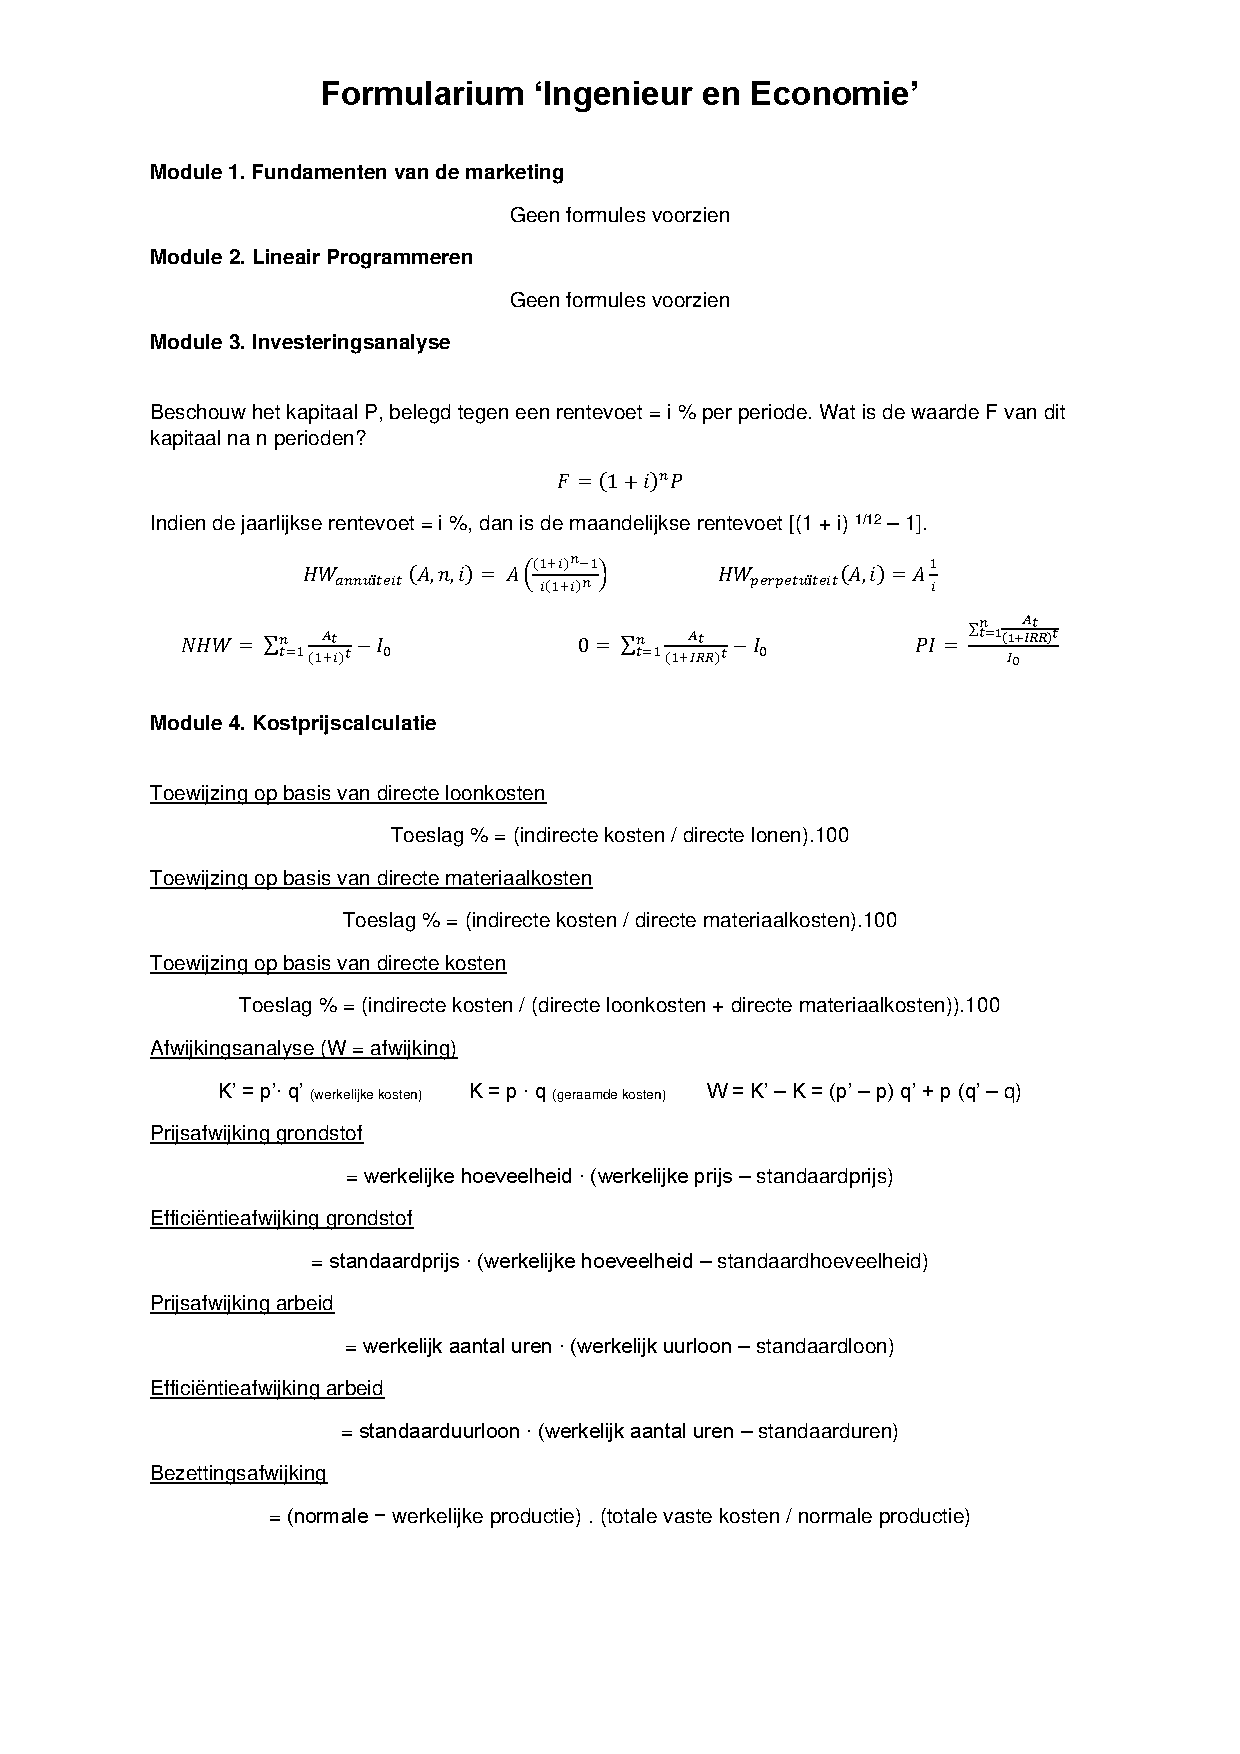
\includepdf[pages=1-2]{Formularium Ingenieur en Economie.pdf}
\printformularium

\section*{Introductie}
\addcontentsline{toc}{section}{Introductie}
Het vak Ingenieur en Economie gaat over marketing,
investeringen, kostenanalyse, prijsbepaling, inflatie en
lineair programmeren. Deze samenvatting bevat de belangrijkste
theorie en oefeningen per module.

\section{Module 1: Marketing}
\subsection{Marketing}

Een markt wordt gedefinieerd met de 4 P's, met nog 2 extra P's die de maatschappij tonen:
\begin{itemize}
    \item Product: Wat wordt er verkocht?
    \item Prijs: Welke prijs wordt er gevraagd?
    \item Plaats: Waar wordt het product verkocht?
    \item Promotie: Hoe wordt het product gepromoot?
    \item Maatschappij (People, Positionering): Wie zijn de klanten en hoe wordt het product gepositioneerd in de markt?
\end{itemize}

De marketingcyclus toont hoe de maatschappij een markt creëert en hoe die markt op zijn beurt weer invloed heeft op de maatschappij.

\begin{enumerate}
    \item \concept{Behoeften, Wensen en Vraag}: Het vertrekpunt is de \textbf{maatschappij},
          die bestaat uit mensen met fundamentele behoeften (fysiek, sociaal, individueel).
          Wanneer deze behoeften gevormd worden door cultuur en persoonlijkheid, spreken we van \textbf{wensen}.
          Als deze wensen gesteund worden door \textbf{koopkracht}, ontstaat er een concrete \textbf{vraag}.
    \item \concept{Producten}: Om aan deze vraag te voldoen, bieden bedrijven \textbf{producten} aan.
          Dit begrip is breed en omvat fysieke goederen, diensten, ervaringen, personen, plaatsen, organisaties en ideeën.
    \item \concept{Waarde, Tevredenheid en Kwaliteit}:
          Als de producten de wens vervullen zijn de behoeftes bevredigd.
          Dit creëert een \textbf{waarde} voor de klant, wat leidt tot \textbf{tevredenheid}.
          De tevredenheid kun je peilen met een tevredenheidsanalyse.
    \item \concept{Kwaliteit}:
          De kwaliteit is de mate waarin een product voldoet aan de verwachtingen van de klant.

    \item \concept{Ruil, Transactie en Relaties}: Een \textbf{ruil} is de kern van marketing: het verkrijgen
          van een gewenst object door iets terug te geven (meestal geld).
          Een \textbf{transactie} is een ruil met meetbare waarden. Succesvolle transacties bouwen langdurige \textbf{relaties} op met klanten.
    \item \concept{Markt}: De verzameling van alle werkelijke en potentiële kopers van een product vormt de
          \textbf{markt}. Deze markt beïnvloedt op zijn beurt weer de maatschappij, waardoor de cyclus rond is.
\end{enumerate}

\begin{figure}[ht]
    \centering
    \begin{tikzpicture}[
            node distance=2cm,
            every node/.style={
                    draw=schoolBlue,
                    thick,
                    rounded corners,
                    align=center,
                    font=\small\bfseries,
                    fill=schoolBlue!5,
                    minimum height=0.8cm,
                    inner sep=6pt
                },
            arrow/.style={->, >=latex, thick, schoolBlue}
        ]
        % Nodes arranged in a circle
        \node (maatschappij) at (0, 4) {Maatschappij};
        \node (behoeften) at (3.5, 3) {Behoeften};
        \node (wensen) at (4.5, 0.5) {Wensen};
        \node (vraag) at (3.5, -2) {Vraag};
        \node (product) at (0, -3) {Product};
        \node (ruil) at (-3.5, -2) {Ruil \&\\Transactie};
        \node (relatie) at (-4.5, 0.5) {Relaties};
        \node (markt) at (-3.5, 3) {Markt};

        % Arrows
        \draw[arrow] (maatschappij) -- (behoeften);
        \draw[arrow] (behoeften) -- (wensen);
        \draw[arrow] (wensen) -- (vraag);
        \draw[arrow] (vraag) -- (product);
        \draw[arrow] (product) -- (ruil);
        \draw[arrow] (ruil) -- (relatie);
        \draw[arrow] (relatie) -- (markt);
        \draw[arrow] (markt) -- (maatschappij);

        % Central text
        \node[draw=none, fill=none] at (0,0.5) {\textcolor{schoolGray}{\textit{Marketingcyclus}}};
    \end{tikzpicture}
    \caption{Schematische weergave van de marketingcyclus}
    \label{fig:marketingcyclus}
\end{figure}
\FloatBarrier % requires \usepackage{placeins} in the preamble

\begin{examenbox}
    Deze cyclus kan exact gevraagd worden op het examen. Ken de stappen goed!
\end{examenbox}

\subsection{Marktmanagement}
Hoe ga je nu je product op de markt brengen?
Marketingmanagement is het proces van het plannen, organiseren, implementeren en controleren van marketingactiviteiten en -strategieën
om organisatiedoelen te bereiken en klantbehoeften te bevredigen. Concreet komt het neer op het strategisch sturen van de vraag naar producten of diensten
(door middel van marketingactiviteiten de behoefte van de klant beïnvloeden) met als doel winstgevende klantrelaties op te bouwen en te behouden.
\newline

Je moet kijken naar de vraag (hoeveel mensen willen het product kopen)
en het aanbod (hoeveel producten zijn er beschikbaar).
\newline

Je wilt relaties opbouwen met de klanten (nieuwe klanten) en bestaande klanten behouden.
Zodat je de maximale waarde uit elke klant haalt (Customer Lifetime Value).
\newline

Flexibel blijven in veranderingen in de markt.


\subsubsection{Marktmanagement concepten}

Er zijn 5 verschillende concepten die je moet kennen!



\begin{tcolorbox}[schoolstyle, title=1. Productieconcept, colframe=schoolBlue!80!black, colback=white]
    \textbf{Uitgangspunt:} Consumenten geven de voorkeur aan producten die beschikbaar en goedkoop zijn. \\
    \textbf{Focus:} Hoge productie-efficiëntie en brede distributie. \\
    \textbf{Wanneer:} Als de vraag groter is dan het aanbod of de productiekost omlaag moet. \\
    \textbf{Gevaar:} Marketing myopia: te veel focus op het proces, te weinig op wat de klant echt nodig heeft. \\
    \textbf{Voorbeeld:} Ford Model T ("Elke kleur, zolang het maar zwart is"), goedkope elektronica.
\end{tcolorbox}

\begin{tcolorbox}[schoolstyle, title=2. Productconcept, colframe=schoolBlue!80!black, colback=white]
    \textbf{Uitgangspunt:} Consumenten willen de beste kwaliteit, prestaties en innovatie. \\
    \textbf{Focus:} Continue productverbetering en technische perfectie. \\
    \textbf{Wanneer:} In markten waar klanten kwaliteit belangrijker vinden dan prijs. \\
    \textbf{Gevaar:} De klant zoekt een oplossing (gat in de muur), geen specifiek product (de boormachine zelf). \\
    \textbf{Voorbeeld:} Apple (design/kwaliteit), high-end audioapparatuur.
\end{tcolorbox}

\begin{tcolorbox}[schoolstyle, title=3. Verkoopconcept, colframe=schoolBlue!80!black, colback=white]
    \textbf{Uitgangspunt:} Consumenten kopen niet genoeg tenzij het bedrijf ze actief overhaalt. \\
    \textbf{Focus:} Grootschalige verkoop- en promotie-inspanningen (Inside-Out). \\
    \textbf{Wanneer:} Bij overcapaciteit of "unsought goods" (waar mensen niet uit zichzelf aan denken). \\
    \textbf{Gevaar:} Focus op transacties in plaats van langdurige klantrelaties; ontevreden klanten na de koop. \\
    \textbf{Voorbeeld:} Verzekeringen, bloeddonatie, agressieve telemarketing.
\end{tcolorbox}

\begin{tcolorbox}[schoolstyle, title=4. Marketingconcept, colframe=schoolBlue!80!black, colback=white]
    \textbf{Uitgangspunt:} Doelen bereiken door de behoeften van de doelgroep beter te vervullen dan de concurrent. \\
    \textbf{Focus:} De klant centraal stellen (Outside-In) en waarde creëren. \\
    \textbf{Wanneer:} In competitieve markten waar de klant keuze heeft (kopersmarkt). \\
    \textbf{Gevaar:} Te veel focus op kleine klantwensen kan innovatie op lange termijn remmen. \\
    \textbf{Voorbeeld:} Coolblue, Amazon, Ikea.
\end{tcolorbox}

\begin{tcolorbox}[schoolstyle, title=5. Maatschappelijk Marketingconcept, colframe=schoolBlue!80!black, colback=white]
    \textbf{Uitgangspunt:} Marketing moet rekening houden met consumentenbehoeften én het welzijn van de samenleving. \\
    \textbf{Focus:} Balans tussen bedrijfswinst, klantwensen en maatschappelijk belang. \\
    \textbf{Wanneer:} Bij groeiend bewustzijn over duurzaamheid, ethiek en gezondheid. \\
    \textbf{Gevaar:} Hogere kosten op korte termijn en complexere besluitvorming. \\
    \textbf{Voorbeeld:} Patagonia, The Body Shop, Fairphone.
\end{tcolorbox}

\begin{examenbox}
    Zorg dat je al deze concepten goed kent en weet wanneer ze toegepast worden en de
    voor- en nadelen van elk concept.
\end{examenbox}

\subsection{Segmentatie}
Je kunt natuurlijk niet iedereen aanspreken met je product. Daarom ga je je markt opdelen in segmenten.
Je kunt groepen opsplitsen op basis van:
\begin{itemize}
    \item Geografisch: Land, regio, stad
    \item Demografisch: Leeftijd, geslacht, inkomen, opleiding
    \item Psychografisch: Levensstijl, persoonlijkheid, waarden
    \item Gedragsmatig: Koopgedrag, merkentrouw, gebruiksfrequentie
\end{itemize}
\begin{figure}[ht]
    \centering
    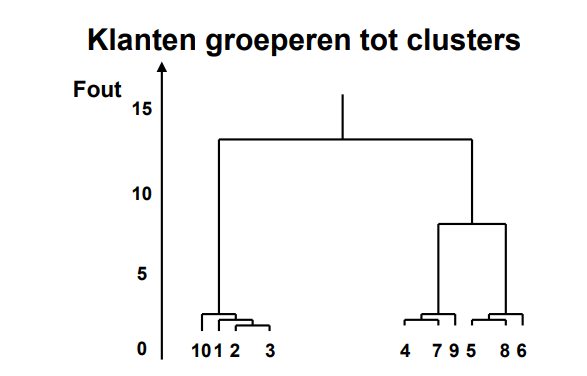
\includegraphics[width=0.5\textwidth]{assets/Clusters.png}
    \caption{Groepen die clusters vormen}
    \label{fig:Clusters.png}
\end{figure}

Je krijgt dan clusters zoals in figuur \ref{fig:Clusters.png}. Waarnaar je heel
gericht kan adverteren.
\subsection{Product Life Cycle}

\begin{examenbox}
    Je moet alle fases kennen en de cyclus kunnen tekenen. De verkoop en de winst.
\end{examenbox}
\begin{figure}[ht]
    \begin{minipage}[t]{0.42\textwidth}
        \vspace{0pt}
        Alle fases zijn:
        \begin{enumerate}
            \item Product development: R\&D, geen verkoop, hoge kosten.
            \item Introductie: Lage verkoop, hoge kosten, geen winst
            \item Groei: Snelle verkoopstijging, dalende kosten, winst begint te komen
            \item Volwassenheid: Verkoop piekt, kosten laag, winst hoog maar begint te dalen
            \item Neergang: Verkoop daalt, kosten stijgen, winst daalt
        \end{enumerate}
    \end{minipage}
    \hfill
    \begin{minipage}[t]{0.55\textwidth}
        \vspace{0pt}
        \centering
        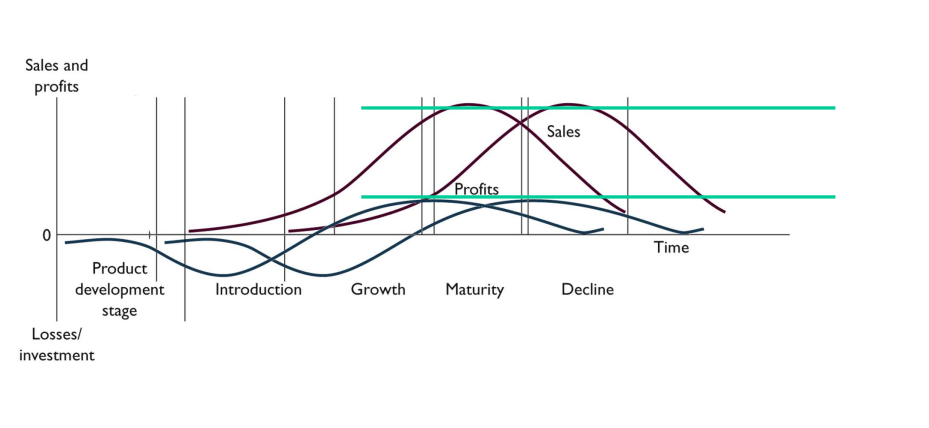
\includegraphics[width=\linewidth]{assets/overlappendePLC's.png}
        \caption{Overlappende PLC's}
        \label{fig:overlappendePLC's.png}
    \end{minipage}
\end{figure}
\FloatBarrier

In de figuur zie je ook dat er overlappende PLC's zijn. Je gaat je
nieuw product lanceren op het einde van de volwassenheidsfase van je vorige product.
Je krijgt dan een positieve winstlijn.

Het \belangrijk{foot-hill effect}: pioneers (early adopters) kopen tijdens de introductiefase al veel,
omdat ze het nieuwste van het nieuwste willen hebben.
Je ziet dan een piek in de verkoop tijdens de introductiefase.
Dit geeft je een vals gevoel van groei omdat deze piek niet blijft duren.


\begin{figure}[htbp]
    \centering
    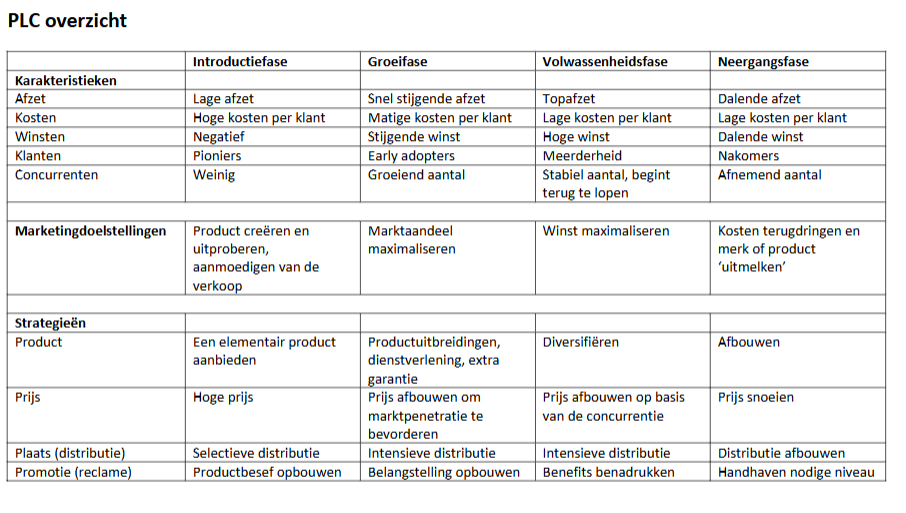
\includegraphics[width=1\textwidth]{assets/tabelplc.png}
    \caption{Tabel met kenmerken van elke PLC fase}
    \label{fig:tabelplc.png}
\end{figure}
\FloatBarrier

Een PLC curve is niet altijd constant en is
afhankelijk van de markt en het product: denk aan \textit{stijl}, \textit{mode} en \textit{rage}.

\begin{figure}[htbp]
    \centering
    \begin{minipage}{0.45\textwidth}
        \textbf{Varianten op de Levenscyclus}
        \begin{description}
            \item[\textcolor{schoolBlue}{Stijl}] Een basis- en onderscheidende wijze van expressie. Gaat generaties mee en golft op en neer in populariteit (bv. formele kleding, koloniale huizen).
            \item[\textcolor{schoolOrange}{Mode}] Een momenteel geaccepteerde of populaire stijl. Groeit langzaam, blijft een tijd populair en daalt dan langzaam (bv. business casual).
            \item[\textcolor{schoolRed}{Rage (Fad)}] Een tijdelijke periode van ongewoon hoge verkoop gedreven door direct consumentenenthousiasme. Stijgt extreem snel, piekt kort, en stort in (bv. Fidget Spinner).
        \end{description}
    \end{minipage}%
    \hfill
    \begin{minipage}{0.5\textwidth}
        \centering
        \begin{tikzpicture}[scale=0.9, >=stealth]
            % Axes
            \draw[->, thick] (0,0) -- (6.5,0) node[right] {\footnotesize Tijd};
            \draw[->, thick] (0,0) -- (0,4.5) node[above] {\footnotesize Verkoop};

            % Stijl (Blue, wavy, long term)
            \draw[schoolBlue, very thick, smooth] plot coordinates {(0,1.5) (1.5,2) (3,1.5) (4.5,2) (6,1.5)};
            \node[schoolBlue, font=\footnotesize, right] at (6,1.5) {Stijl};

            % Mode (Orange, bell curve)
            \draw[schoolOrange, very thick] (0.5,0.5) .. controls (2.5,0.5) and (2.5,3.5) .. (3.5,3.5) .. controls (4.5,3.5) and (4.5,0.5) .. (6,0.5);
            \node[schoolOrange, font=\footnotesize] at (3.5, 3.8) {Mode};

            % Rage (Red, spike)
            \draw[schoolRed, very thick] (0.5,0) -- (1,0) -- (1.5, 4) -- (2,0) -- (6,0);
            \node[schoolRed, font=\footnotesize] at (1.5, 4.3) {Rage};
        \end{tikzpicture}
        \caption{Visueel verloop van PLC varianten}
        \label{fig:plc_types}
    \end{minipage}
\end{figure}


\subsection{Prijszetting}

Hoe ga je de prijs van je product bepalen?
Je hebt interne en externe factoren die de prijszetting beïnvloeden.
Interne factoren zijn factoren binnen het bedrijf zelf \textit{(bijv. kosten, marketingdoelstellingen, marketingmix strategie, organisatieverantwoordelijkheid)},
terwijl externe factoren buiten het bedrijf liggen \textit{(bijv. concurrentie, markttrends, economische omstandigheden, omgeving)}.

\subsubsection{Interne factoren}
De prijszetting wordt beïnvloed door vier belangrijke interne factoren:

\begin{figure}[ht]
    \centering
    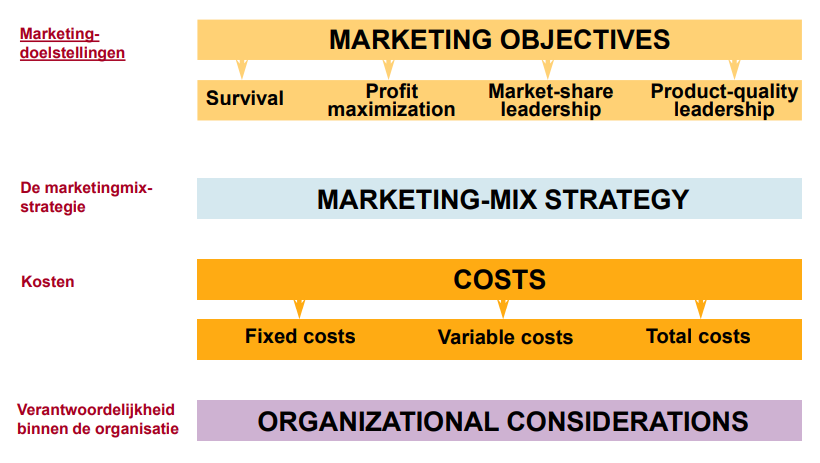
\includegraphics[width=0.7\textwidth]{assets/internefactoren.png}
    \caption{Interne factoren die de prijszetting beïnvloeden}
    \label{fig:internefactoren.png}
\end{figure}
\FloatBarrier

\begin{description}
    \item\concept{Marketingdoelstellingen} Voordat de prijs wordt bepaald, moet het bedrijf zijn strategie kiezen:
          \begin{itemize}
              \item \textbf{Overleven:} Bij overcapaciteit of hevige concurrentie; lage prijzen om de productie draaiende te houden.
              \item \textbf{Winstmaximalisatie:} Prijzen zo kiezen dat de huidige winst maximaal is (korte termijn focus).
              \item \textbf{Marktaandeel leiderschap:} Zo laag mogelijke prijzen om snel een groot marktaandeel te veroveren.
              \item \textbf{Kwaliteitsleiderschap:} Hoge prijzen om R\&D en hoge kwaliteit te dekken.
          \end{itemize}

    \item\concept{Marketingmix strategie} De prijs moet overeenkomen met de andere P's van de marketingmix:
          \begin{itemize}
              \item \textbf{Plaats:} \textit{bijv. Exclusieve distributie vereist vaak hogere prijzen.}
              \item \textbf{Promotie:} \textit{bijv. Intensieve promotiecampagnes kunnen hogere prijzen rechtvaardigen.}
              \item \textbf{Product:} \textit{bijv. Premium producten kunnen hogere prijzen vragen dan basisproducten.}
          \end{itemize}

    \item\concept{Kosten} De kosten bepalen de \textbf{bodemprijs} (vloer).
          Het bedrijf moet een prijs vragen die de vaste en variabele kosten dekt en een eerlijk rendement oplevert.
          \begin{itemize}
              \item \textbf{Vaste kosten:} Kosten die niet variëren met productie (huur, rente, salarissen).
              \item \textbf{Variabele kosten:} Kosten die direct variëren met het productieniveau.
              \item \textbf{Totale kosten:} $TK = TCK + TVK$\\
                    met $TK$ de totale kosten, $TCK$ de totale constante (vaste) kosten
                    en $TVK$ de totale variabele kosten.
          \end{itemize}


    \item\concept{Verantwoordelijkheid binnen de organisatie}
          Wie bepaalt de prijs binnen het bedrijf?
          \textit{Management, verkoopteam, marketingafdeling, financieel team.}
\end{description}

Om de prijs te meten kun je een prijsvork gebruiken.
\begin{figure}[ht]
    \centering
    \begin{minipage}{0.45\textwidth}
        \textbf{De Prijsvork: Klantperceptie}\\
        De prijsvork wordt bepaald door de perceptie van de klant. Er is een range van aanvaardbare prijzen:
        \begin{itemize}
            \item \textbf{Te laag:} De klant vertrouwt de kwaliteit niet.
            \item \textbf{Te hoog:} De klant vindt het product het geld niet waard.
            \item \textbf{Acceptabel:} De zone hiertussen waar de aankoopwaarschijnlijkheid het grootst is.
        \end{itemize}
    \end{minipage}%
    \hfill
    \begin{minipage}{0.55\textwidth}
        \centering
        \begin{tikzpicture}[scale=0.85, >=stealth]
            % Axis
            \draw[->, thick] (0,0) -- (8,0) node[right] {Prijs (€)};

            % Zones
            % Te Goedkoop
            \fill[schoolRed!30] (0,0.2) rectangle (2.5,1.2);
            \node[font=\scriptsize, align=center] at (1.25, 0.7) {Te\\Goedkoop};

            % Acceptabel
            \fill[schoolBlue!30] (2.5,0.2) rectangle (5.5,1.2);
            \node[font=\footnotesize, align=center, font=\bfseries] at (4, 0.7) {Aanvaardbare\\Prijsrange};

            % Te Duur
            \fill[schoolRed!30] (5.5,0.2) rectangle (8,1.2);
            \node[font=\scriptsize, align=center] at (6.75, 0.7) {Te\\Duur};

            % Inputs markers (boven de balken)
            \draw[thick, schoolBlue] (2.5,1.2) -- (2.5,1.8) node[above, font=\tiny, align=center] {Min. grens\\(Kwaliteit)};
            \draw[thick, schoolBlue] (5.5,1.2) -- (5.5,1.8) node[above, font=\tiny, align=center] {Max. grens\\(Budget)};

            % Customers (dots representing input) onder de as
            \foreach \x in {2.7, 3, 3.5, 4, 4.5, 5, 5.3}
            \fill[schoolGray] (\x, -0.3) circle (1.5pt);
            \node[right, font=\tiny, schoolGray] at (5.5, -0.3) {Klant input};

        \end{tikzpicture}
    \end{minipage}
\end{figure}
\FloatBarrier

\subsubsection{Externe factoren}
Externe factoren
zijn factoren die niet door het bedrijf zelf kunnen worden beïnvloed,
maar die wel een grote impact hebben op de prijszetting.

\begin{figure}[ht]
    \centering
    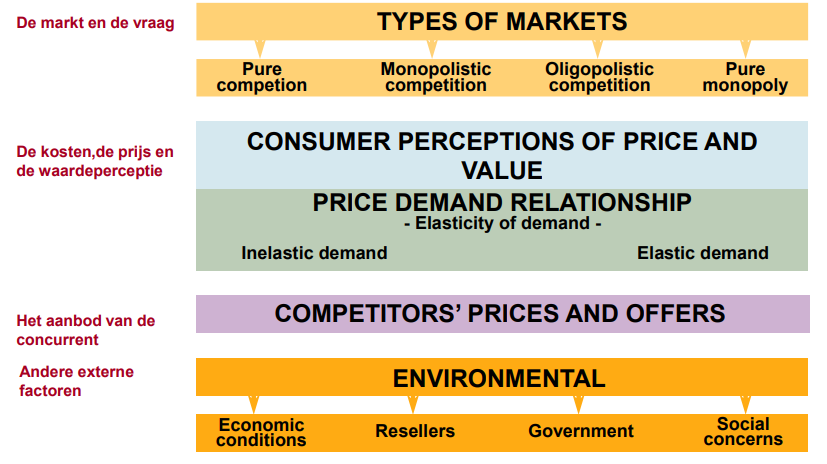
\includegraphics[width=0.7\textwidth]{assets/externe factoren.png}
    \caption{Externe factoren die de prijszetting beïnvloeden}
    \label{fig:externfactoren.png}
\end{figure}
\FloatBarrier

\begin{description}
    \item\concept{De Markt en Concurrentie}
          In welke markt opereer je? De vrijheid om je prijs te zetten (pricing power) hangt sterk af van de concurrentievorm. In een zeer competitieve markt bepaalt de markt de prijs, terwijl je in een monopolie zelf de prijs kunt zetten.

          \begin{figure}[ht]
              \centering
              \begin{tikzpicture}[scale=0.85, >=stealth]
                  % Main Arrow
                  \draw[->, ultra thick, schoolGray] (0,0) -- (13,0) node[right, align=left, font=\footnotesize] {\textbf{Pricing Power}\\\textit{(Invloed op prijs)}};

                  % Nodes (Boxes)
                  % 1. Volledige Mededinging
                  \node[fill=schoolBlue!10, draw=schoolBlue, rounded corners, minimum width=2.8cm, minimum height=1cm, align=center, font=\footnotesize] (vol) at (1.5, 1.5) {\textbf{Volledige}\\\textbf{Mededinging}};
                  \draw[-, thick, schoolBlue] (1.5, 0.1) -- (1.5, 1);
                  \node[below, font=\scriptsize, align=center, text width=2.5cm] at (1.5, -0.2) {Veel aanbieders\\Homogeen product\\\textit{Vb: Graan, Melk}};

                  % 2. Monopolistische Concurrentie
                  \node[fill=schoolBlue!20, draw=schoolBlue, rounded corners, minimum width=2.8cm, minimum height=1cm, align=center, font=\footnotesize] (moncon) at (4.7, 1.5) {\textbf{Monopolistische}\\\textbf{Concurrentie}};
                  \draw[-, thick, schoolBlue] (4.7, 0.1) -- (4.7, 1);
                  \node[below, font=\scriptsize, align=center, text width=2.5cm] at (4.7, -0.2) {Veel aanbieders\\Gedifferentieerd\\\textit{Vb: Kleding, Horeca}};

                  % 3. Oligopolie
                  \node[fill=schoolOrange!20, draw=schoolOrange, rounded corners, minimum width=2.8cm, minimum height=1cm, align=center, font=\footnotesize] (oli) at (7.9, 1.5) {\textbf{Oligopolie}};
                  \draw[-, thick, schoolOrange] (7.9, 0.1) -- (7.9, 1);
                  \node[below, font=\scriptsize, align=center, text width=2.5cm] at (7.9, -0.2) {Weinig aanbieders\\Hoge drempels\\\textit{Vb: Telecom, Banken}};

                  % 4. Monopolie
                  \node[fill=schoolRed!20, draw=schoolRed, rounded corners, minimum width=2.8cm, minimum height=1cm, align=center, font=\footnotesize] (mon) at (11.1, 1.5) {\textbf{Monopolie}};
                  \draw[-, thick, schoolRed] (11.1, 0.1) -- (11.1, 1);
                  \node[below, font=\scriptsize, align=center, text width=2.5cm] at (11.1, -0.2) {Eén aanbieder\\Uniek product\\\textit{Vb: Waterbedrijf}};

              \end{tikzpicture}
              \caption{Het spectrum van marktconcurrentie: van prijsnemer naar prijszetter}
              \label{fig:market_spectrum}
          \end{figure}
          \FloatBarrier % requires \usepackage{placeins} in the preamble

    \item\concept{Consumentenperceptie van waarde}
          Uiteindelijk bepaalt de consument of de prijs gerechtvaardigd is.
          Een belangrijk concept hierbij is de \textbf{prijselasticiteit} $E_p$: hoe sterk reageert de vraag op een prijsverandering?
          \[ E_p = \frac{\%\Delta Q}{\%\Delta P} \]
          met $E_p$ de prijselasticiteit van de vraag, $\%\Delta Q$ de procentuele verandering in gevraagde hoeveelheid
          en $\%\Delta P$ de procentuele verandering in prijs.
          Is $|E_p| > 1$ dan is de vraag \textbf{elastisch} (de hoeveelheid reageert sterker dan de prijs);
          is $|E_p| < 1$ dan is ze \textbf{inelastisch}.

          \begin{figure}[ht]
              \centering
              \begin{minipage}{0.45\textwidth}
                  \centering
                  \begin{tikzpicture}[scale=0.7, >=stealth]
                      \draw[->, thick] (0,0) -- (4,0) node[right] {Q};
                      \draw[->, thick] (0,0) -- (0,4) node[above] {P};
                      \draw[thick, schoolBlue] (1,3.5) -- (2.5,0.5) node[midway, right] {D};
                      \node[align=center, font=\bfseries\small] at (2,4) {Inelastisch};
                      % Change
                      \draw[dashed] (0,3) -- (1.2,3) -- (1.2,0);
                      \draw[dashed] (0,1.5) -- (2,1.5) -- (2,0);

                      \draw[<->, schoolRed] (0.2,1.5) -- (0.2,3) node[midway, left, font=\tiny] {$\Delta P$};
                      \draw[<->, schoolRed] (1.2,0.2) -- (2,0.2) node[midway, below, font=\tiny] {$\Delta Q$};
                  \end{tikzpicture}
                  \caption*{Steile curve: $\Delta P > \Delta Q$}
              \end{minipage}
              \hfill
              \begin{minipage}{0.45\textwidth}
                  \centering
                  \begin{tikzpicture}[scale=0.7, >=stealth]
                      \draw[->, thick] (0,0) -- (4,0) node[right] {Q};
                      \draw[->, thick] (0,0) -- (0,4) node[above] {P};
                      \draw[thick, schoolBlue] (0.5,3) -- (3.5,1) node[midway, above right] {D};
                      \node[align=center, font=\bfseries\small] at (2,4) {Elastisch};

                      % Change
                      \draw[dashed] (0,2.5) -- (1.2,2.5) -- (1.2,0);
                      \draw[dashed] (0,1.8) -- (2.3,1.8) -- (2.3,0);

                      \draw[<->, schoolRed] (0.2,1.8) -- (0.2,2.5) node[midway, left, font=\tiny] {$\Delta P$};
                      \draw[<->, schoolRed] (1.2,0.2) -- (2.3,0.2) node[midway, below, font=\tiny] {$\Delta Q$};
                  \end{tikzpicture}
                  \caption*{Vlakke curve: $\Delta P < \Delta Q$}
              \end{minipage}
              \caption{Prijselasticiteit van de vraag}
              \label{fig:elasticity}
          \end{figure}
          \FloatBarrier

    \item\concept{Competitie binnen je markt}
          Wat zijn de prijzen van je concurrenten en hun offering?

    \item\concept{Omgevingsfactoren}
          Verschillende externe omgevingsfactoren kunnen de prijszetting beïnvloeden:

          \begin{description}
              \item [Economische omstandigheden:] Inflatie, recessie, koopkracht.
              \item [Sociale en culturele factoren:] Trends, normen, waarden.
              \item [Wet- en regelgeving:] Prijscontroles, belastingen, handelsbeperkingen.
              \item [Herverkopers en distributiekanalen:] zoals groothandels en winkels, bijvoorbeeld Bol.com of Amazon.
          \end{description}
\end{description}

\begin{examenbox}
    Leg jezelf niet te veel druk op om deze exacte factoren te onthouden.
    Begrijp wel hoe interne en externe factoren de prijszetting beïnvloeden.
\end{examenbox}

\subsubsection{Alles samen}
Als al deze factoren zijn overwogen, kan het bedrijf een prijsstrategie ontwikkelen die
past bij zijn marketingdoelstellingen en de marktomstandigheden.
\newline

Een bedrijf kiest dan een strategie afhankelijk van de prijs en de kwaliteit van het product:


\noindent
\begin{minipage}[t]{0.45\textwidth}
    \begin{itemize}
        \item \textbf{Hoge prijs, hoge kwaliteit:} Premiumstrategie
        \item \textbf{Hoge prijs, lage kwaliteit:} Overgeprijsd
        \item \textbf{Lage prijs, hoge kwaliteit:} Good-value-strategie
        \item \textbf{Lage prijs, lage kwaliteit:} Economystrategie
    \end{itemize}
\end{minipage}
\hfill
\begin{minipage}[t]{0.5\textwidth}
    \centering
    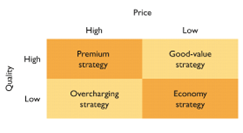
\includegraphics[width=1\textwidth]{assets/image5.png}
\end{minipage}



\subsection{Prijszettingsmethodes}



\subsubsection{Nieuwe producten}

\textbf{Afroomstrategie:} Je zet een hoge prijs
in het begin en verlaagt die dan geleidelijk.
Dit werkt goed als je al een gevestigde reputatie hebt en je product
uniek is. Early adopters zijn bereid meer te betalen voor het nieuwste product.
\newline

\textbf{Penetratiestrategie:} Je zet een lage prijs om snel marktaandeel te veroveren.
Daarna verhoog je de prijs.
Dit werkt goed in een competitieve markt.


\subsubsection{Assortiment producten}
Dit zijn producten in groep of deals die je aanbiedt.

\begin{itemize}
    \item \textbf{Productlijn-prijszetting:} Je zet vaste prijsstappen tussen de producten in één lijn \textit{(laptops, smartphones)}.
    \item \textbf{Optie-prijszetting:} Accessoires of extra's worden apart geprijsd. \textit{auto's met extra opties}.
    \item \textbf{Captive-prijszetting:} Je verkoopt een basisproduct tegen een lage prijs, maar de bijbehorende
          verbruiksartikelen zijn duur \textit{Scheermesjes en cartridges}.
    \item \textbf{By-product-prijszetting:} Je verkoopt bijproducten
          om de kosten van het hoofdproduct te compenseren. \textit{vlees en leer}.
    \item \textbf{Productbundel-prijszetting:} Je verkoopt meerdere producten
          samen tegen een lagere prijs
\end{itemize}


\subsection{Prijsaanpasstrategieën}
Prijzen zijn natuurlijk niet altijd hetzelfde. Er zijn kortingen, deals, seizoensprijzen etc.
Of prijzen worden aangepast om het als een betere deal te laten lijken (€9,99 in plaats van €10).
\begin{itemize}
    \item \textbf{Korting en bonussen:} Prijsverlagingen voor vroege betalingen, grote bestellingen of seizoensgebonden aankopen.
    \item \textbf{Segmentatie-prijszetting:} Verschillende prijzen voor verschillende klantsegmenten \textit{(studenten, senioren)}.
    \item \textbf{Psychologische prijszetting:} Prijzen die psychologisch aantrekkelijk zijn \textit{(bijv. €9,99 in plaats van €10)}.
    \item \textbf{Promotionele prijszetting:} Tijdelijke prijsverlagingen om de verkoop te stimuleren \textit{(kortingen, coupons)}.
    \item \textbf{Geografische prijszetting:} Prijzen variëren op basis van locatie \textit{(exportprijzen, lokale marktomstandigheden)}.
    \item \textbf{Internationale prijszetting:} Prijzen worden aangepast voor verschillende landen op basis van economische omstandigheden, concurrentie,
          invoertarieven\dots
\end{itemize}


\section{Module 2: Lineair Programmeren}

Lineair programmeren (LP) is een wiskundige methode om de
beste uitkomst (zoals maximale winst of laagste kosten) te bepalen
wanneer je lineaire relaties hebt.

Hieronder een voorbeeld
waarbij je twee producten maakt met verschillende winstbijdragen
maar je bent beperkt in grondstoffen en tijd.

\begin{figure}[ht]
    \centering
    \begin{minipage}{0.45\textwidth}
        \textbf{Kernbegrippen van LP}
        \begin{description}
            \item[\concept{Doelfunctie:}] Wat wil je
                  optimaliseren of maximaliseren? (bijv. winst, kosten)
                  \[\max Z = c_1 x_1 + c_2 x_2\]
            \item[\concept{Beperkingen:}] De limieten waarbinnen
                  je moet werken (tijd, budget, grondstoffen).
                  Deze vormen lijnen in de grafiek.
                  \[\text{Beperking }1:\quad a_{11}x_1 + a_{12}x_2 \leq b_1\]
        \end{description}
    \end{minipage}%
    \hfill
    \begin{minipage}{0.5\textwidth}
        \centering
        \begin{tikzpicture}[scale=0.85, >=stealth]
            % Grid
            \draw[help lines, color=gray!20] (0,0) grid (7,6);

            % Assen
            \draw[->, thick] (0,0) -- (7,0) node[right] {$x_1$};
            \draw[->, thick] (0,0) -- (0,6.5) node[above] {$x_2$};

            % Beperking 1: (0,5) naar (5,0) -> x + y <= 5
            \draw[thick, schoolRed!80] (0,5) -- (5.5, -0.5);
            \node[schoolRed!80, font=\footnotesize, right] at (0.2, 5) {Beperking 1};

            % Beperking 2: (0,3) naar (6,0) -> x + 2y <= 6
            \draw[thick, schoolOrange!80] (0,3) -- (6.5, -0.25);
            \node[schoolOrange!80, font=\footnotesize, right] at (0.2, 3.2) {Beperking 2};

            % Toegelaten gebied (polygon)
            \fill[schoolBlue, opacity=0.15] (0,0) -- (5,0) -- (4,1) -- (0,3) -- cycle;
            \node[schoolBlue!80!black, font=\bfseries\small, align=center] at (2, 1.2) {Toegelaten\\Gebied};

            % Optimale oplossing (snijpunt 4,1)
            \fill[schoolBlue] (4,1) circle (3pt);

            % Pijl naar optimum (in vrije ruimte)
            \draw[<-, thick, schoolBlue] (4.1, 1.1) -- (5.5, 3.5) node[right, align=left] {\textbf{Optimum}\\(Max Winst)};

            % Winstlijn (stippellijn) Z = x + y (loodrecht op vector (1,1))
            % Door punt (4,1): x+y=5. Lijn (2,3) tot (5,0)
            \draw[dashed, thick, schoolGray] (2,3) -- (6, -1);
            \node[schoolGray, font=\footnotesize, rotate=-45] at (3, 2.2) {Winstlijn};

        \end{tikzpicture}
        \caption{Grafische oplossing van een LP-probleem}
        \label{fig:lp_graph}
    \end{minipage}
\end{figure}

Als je moet bepalen hoe je het meeste winst
maakt afhankelijk van verschillende producten en beperkingen,
dan gebruik je lineair programmeren. De grafische methode werkt goed voor 2 variabelen;
voor meer variabelen gebruik je de Simplex-methode.

\subsection{Simplex Methode}

\begin{enumerate}
    \item \textbf{Standaardvorm:} Zet alle ongelijkheden ($\leq$) om in vergelijkingen (=) door Slack Variabelen (s) toe te voegen.
          Slack vangt het ongebruikte deel van een middel op.
    \item \textbf{Start:} Begin in de oorsprong (alles 0).
    \item \textbf{Iteratie (Pivoteren):}
          \begin{enumerate}
              \item Kies de binnenkomende variabele (Entering Variable): Kijk naar de doelfunctie-rij. Welke variabele heeft de meest negatieve coëfficiënt? Die levert de meeste winststijging op.
              \item Kies de uitgaande variabele (Leaving Variable): Doe de Minimum Ratio Test (Rechterzijde / Binnenkomende kolom). De kleinste positieve ratio wint. Dit is de beperking die je als eerste raakt (de flessenhals).
              \item Update: Reken de tabel om zodat de nieuwe variabele in de basis komt en de oude eruit gaat.
          \end{enumerate}
    \item \textbf{Stop:} Als er geen negatieve getallen meer in de doelfunctie-rij staan, heb je het optimum bereikt
\end{enumerate}

\subsection{Simplex Methode: Voorbeeld}
Stel we produceren twee producten ($x_1$ en $x_2$). Elk product vereist een bepaalde tijd voor assemblage en elektronica. We willen de winst ($P$) maximaliseren.

\textbf{Gegevens:}
\begin{itemize}
    \item \textbf{Doelfunctie:} Max $P = 7x_1 + 5x_2$
    \item \textbf{Beperkingen:}
          \begin{itemize}
              \item Assemblage tijd: $4x_1 + 3x_2 \leq 240$
              \item Elektronica tijd: $2x_1 + 1x_2 \leq 100$
          \end{itemize}
\end{itemize}

\textbf{Stap 1: Slack Variabelen toevoegen} \\
Om de ongelijkheden ($\leq$) op te lossen met een matrix, moeten we ze omzetten naar vergelijkingen ($=$). Hiervoor introduceren we \textbf{slackvariabelen} ($S_1$ en $S_2$).
\begin{itemize}
    \item $S_1$: De ongebruikte tijd in de assemblage-afdeling. Als $S_1 > 0$, hebben we tijd over.
    \item $S_2$: De ongebruikte tijd in de elektronica-afdeling.
\end{itemize}
De vergelijkingen worden dan:
\begin{align*}
    4x_1 + 3x_2 + 1S_1 + 0S_2     & = 240 \\
    2x_1 + 1x_2 + 0S_1 + 1S_2     & = 100 \\
    P - 7x_1 - 5x_2 - 0S_1 - 0S_2 & = 0
\end{align*}

\textbf{Stap 2: Initiële Simplex Tabel} \\
We zetten dit in een matrix. De onderste rij is de doelfunctie.

\begin{table}[H]
    \centering
    \caption{Initiële Simplex Tableau}
    \begin{tabular}{lcccccc}
        \toprule
        \textbf{Basis} & $\mathbf{P}$ & $\mathbf{x_1}$ & $\mathbf{x_2}$ & $\mathbf{S_1}$ & $\mathbf{S_2}$ & \textbf{Oplossing} \\
        \midrule
        $S_1$          & 0            & \textbf{4}     & 3              & 1              & 0              & 240                \\
        $S_2$          & 0            & 2              & 1              & 0              & 1              & 100                \\
        \midrule
        $P$            & 1            & -7             & -5             & 0              & 0              & 0                  \\
        \bottomrule
    \end{tabular}
\end{table}

\textbf{Stap 3: Oplossen (Rij-operaties)} \\
We voeren rij-operaties (vegen) uit totdat er geen negatieve getallen meer staan in de onderste rij.
\begin{enumerate}
    \item \textbf{Pivot Kolom:} Meest negatieve waarde in rij $P$ is $-7$ (dus variabele $x_1$ moet de basis in).
    \item \textbf{Pivot Rij:} We delen de oplossing door de pivot-kolom: $240/4 = 60$ en $100/2 = 50$. De kleinste waarde is 50, dus rij $S_2$ is de pivot rij.
    \item \textbf{Vegen:} We maken van de pivot (positie $S_2, x_1$) een 1 en zorgen dat de andere waarden in die kolom 0 worden.
\end{enumerate}
Na het uitvoeren van alle iteraties krijgen we de eindtabel:

\begin{table}[H]
    \centering
    \caption{Simplex Tableau: Oplossing}
    \begin{tabular}{lcccccc}
        \toprule
        \textbf{Basis} & $\mathbf{P}$ & $\mathbf{x_1}$ & $\mathbf{x_2}$ & $\mathbf{S_1}$ & $\mathbf{S_2}$ & \textbf{Oplossing} \\
        \midrule
        $x_2$          & 0            & 0              & 1              & 1              & -2             & 40                 \\
        $x_1$          & 0            & 1              & 0              & -0.5           & 1.5            & 30                 \\
        \midrule
        $P$            & 1            & 0              & 0              & 1.5            & 0.5            & \textbf{410}       \\
        \bottomrule
    \end{tabular}
\end{table}

\textbf{Conclusie en Interpretatie:} \\
In de kolom "Oplossing" lezen we de optimale waarden af voor de \textbf{basisvariabelen} ($x_1, x_2, P$).
Variabelen die \textbf{niet} in de kolom `Basis' staan (hier $S_1$ en $S_2$), zijn \textbf{niet-basisvariabelen}
en hebben per definitie de waarde \textbf{0}.

\begin{itemize}
    \item $\mathbf{x_1 = 30}$: We produceren 30 eenheden van product 1.
    \item $\mathbf{x_2 = 40}$: We produceren 40 eenheden van product 2.
    \item $\mathbf{P = 410}$: De maximale winst is 410.
    \item $S_1 = 0$ en $S_2 = 0$: Dit betekent dat er geen ongebruikte tijd is.
          \begin{itemize}
              \item Assemblage: $4(30) + 3(40) = 120 + 120 = 240$ uur gebruikt (van de 240).
              \item Elektronica: $2(30) + 1(40) = 60 + 40 = 100$ uur gebruikt (van de 100).
          \end{itemize}
          Beide afdelingen draaien dus op volle capaciteit (bottlenecks).
\end{itemize}

\subsection{Sensitiviteitsanalyse}

In de praktijk veranderen dingen. De winstmarges kunnen stijgen of dalen. Je krijgt meer of minder materiaal. Wat gebeurt er met je optimale plan? Moet je alles opnieuw berekenen?

Sensitiviteitsanalyse geeft antwoord: \textbf{Hoeveel mag iets veranderen voordat je plan niet meer werkt?}

\subsubsection{A. Wat als de winst per product verandert?}

\begin{theorieblok}[Doelfunctie-coëfficiënten]
    De coëfficiënten in de doelfunctie zijn de winstbedragen per product (bijv. €7 per product A, €5 per product B).
\end{theorieblok}

Stel je wint nu €7 op product A. Maar morgen stijgt de vraag en kun je €8 vragen.

\textbf{Wat gebeurt er?} De winstlijn kantelt. Je gaat meer product A maken.

\textbf{Hoeveel mag veranderen?} Tot ongeveer een bepaald punt. Als je €9 per product A kunt vragen, is het misschien niet meer winstgevend om product B te maken. Dan maak je enkel product A.

\begin{itemize}
    \item \textbf{Binnen de grens:} Je houdt dezelfde producten. Alleen je totale winst stijgt of daalt.
    \item \textbf{Voorbij de grens:} Je schakelt over naar een ander productieplan. Je moet opnieuw bekijken wat je maakt.
\end{itemize}

\subsubsection{B. Wat als je meer of minder materiaal hebt?}

\begin{theorieblok}[Rechterzijde van beperkingen (RHS)]
    Beperkingen hebben getallen aan de rechterkant: "Assemblage $\leq$ 240 uur". Die 240 is de rechterzijde.
\end{theorieblok}

Stel je hebt 240 uur assemblagewerk. Nu krijg je een stagiair: plots heb je 270 uur.

\textbf{Wat gebeurt er?} Je kunt meer producten maken.
Je winstgrens schuift omhoog. Maar misschien wordt elektronica nu de bottleneck in plaats van assemblage.

\textbf{Hoeveel mag veranderen?} Tot een andere beperking bindend wordt. Ga je van 240 naar 180 uur, dan wordt assemblage zo krap dat de basis wisselt: een ander productieplan wordt optimaal en de oude schaduwprijs geldt niet meer.

\begin{itemize}
    \item \textbf{Binnen de grens:} Hetzelfde plan werkt. Je maakt gewoon meer of minder stukken.
    \item \textbf{Voorbij de grens:} Een ander hulpmiddel (machine, tijd, grondstof) wordt nu het probleem. Je plan valt in duigen.
\end{itemize}

\subsubsection{C. Hoeveel waard is één extra eenheid?}

\begin{theorieblok}[Schaduwprijs (Shadow Price)]
    Dit is: hoeveel extra winst je krijgt als je één eenheid extra krijgt van iets wat beperkt is.
\end{theorieblok}

Je hebt precies genoeg assemblagewerk (240 uur). Je bent dus volledig aan het werk.

Vraag: \textbf{Hoeveel zou het je waard zijn om 1 extra uur assemblage te hebben?}

Antwoord: Als je schaduwprijs €5 is, levert 1 extra uur €5 extra winst op.

\textbf{Praktisch voorbeeld:}
\begin{itemize}
    \item Je schaduwprijs voor assemblage = €5 per uur.
    \item Een uur huren van iemand anders kost €3.
    \item \textbf{Doe het!} Je verdient €5 en betaalt €3. Netto €2 winst.
    \item Maar als huren €6 kost?
    \item \textbf{Niet doen!} Je verdient €5 maar betaalt €6. Je verliest €1.
\end{itemize}

\textbf{Belangrijk:} Schaduwprijzen werken alleen als je al volledig aan het werk bent (geen overschot). Als je nog grondstof over hebt, is de schaduwprijs €0 (meer ervan helpt niet).

\begin{description}
    \item[Schaduwprijs:]
          De waarde van één extra eenheid van iets wat beperkt is (hulpbron, grondstof, tijd).
    \item[Bereik:]
          Binnen dit bereik blijft je schaduwprijs geldig.
    \item[Verandering:]
          Als dingen veel veranderen, verandert je hele plan.
\end{description}


\begin{oefenblok}[Oefening 1: Verandering in Winstmarges]
    Context: Een bedrijf maakt mountainbikes ($x_1$) en racefietsen ($x_2$).
    Huidig optimaal plan: 2 mountainbikes, 2 racers. Totale winst: \$50.

    \textbf{Vraag A:} De marketingafdeling meldt dat door een promotie de winst op een Mountainbike ($x_1$) daalt van \$15 naar \$11.
    \begin{itemize}
        \item Blijft ons huidige productieplan (2 mountainbikes, 2 racers) optimaal?
        \item Wat is de nieuwe totale winst?
    \end{itemize}

    \textbf{Gegeven uit sensitivity analyse:}
    \begin{itemize}
        \item Huidige winst mountainbike: \$15
        \item Allowable Decrease: \$5
    \end{itemize}

    \textbf{Oplossing:}
    \begin{enumerate}
        \item \textbf{Bereken de verandering:} De daling is $15 - 11 = 4$
        \item \textbf{Vergelijk met toegestane range:}
              Omdat de daling (4) kleiner is dan de toegestane daling (5), verandert de basis niet.
        \item \textbf{Conclusie:} We produceren nog steeds dezelfde aantallen ($x_1 = 2, x_2 = 2$)
        \item \textbf{Nieuwe Winst:}
              \begin{align*}
                  Z_{\text{nieuw}} & = (11 \times 2) + (10 \times 2) \\
                                   & = 22 + 20 = \$42
              \end{align*}
              Alternatief: Oude winst (50) - daling $(4 \times 2 \text{ fietsen}) = \$42$
    \end{enumerate}

    \vspace{5mm}

    \textbf{Vraag B:} De winst op een Racefiets ($x_2$) stijgt plotseling naar \$20. Blijven we hetzelfde doen?

    \textbf{Gegeven:}
    \begin{itemize}
        \item Huidige winst racefiets: \$10
        \item Allowable Increase: \$5
    \end{itemize}

    \textbf{Oplossing:}
    \begin{enumerate}
        \item \textbf{Bereken de verandering:} De stijging is $20 - 10 = 10$
        \item \textbf{Vergelijk met toegestane range:}
              De stijging (10) is groter dan de toegestane stijging (5)
        \item \textbf{Conclusie:} We vallen \textbf{buiten de range}. Het huidige productieplan is niet langer optimaal.
              We moeten het model opnieuw oplossen (waarschijnlijk wordt het interessanter om meer racefietsen te maken ten koste van mountainbikes).
    \end{enumerate}
\end{oefenblok}

\begin{oefenblok}[Oefening 2: Verandering in Beperkingen (Shadow Prices)]
    Context: Zelfde bedrijf. De productie wordt beperkt door machinecapaciteit (Metal Finishing).

    \textbf{Gegeven uit sensitivity analyse:}
    \begin{itemize}
        \item Shadow Price voor machinecapaciteit: \$10
        \item Allowable Increase: 1 uur
    \end{itemize}

    \textbf{Vraag C:} Je krijgt de kans om 1 uur extra machinecapaciteit te huren bij de buren.
    De buurman vraagt hiervoor \$8. Moet je dit doen?

    \textbf{Oplossing:}
    \begin{enumerate}
        \item \textbf{Betekenis Shadow Price:} 1 extra uur levert ons \$10 extra winst op (zolang we binnen de range blijven)
        \item \textbf{Check de range:} We voegen 1 uur toe. De Allowable Increase is 1.
              We zitten dus precies op de grens, maar het mag nog net.
        \item \textbf{Berekening:}
              \begin{itemize}
                  \item Opbrengst van extra uur: \$10
                  \item Kosten van extra uur: \$8
                  \item Netto winst: $10 - 8 = \$2$
              \end{itemize}
        \item \textbf{Conclusie:} \textbf{Ja}, je moet dit doen. Het verhoogt de totale winst van het bedrijf met \$2.
    \end{enumerate}

    \vspace{5mm}

    \textbf{Vraag D:} Stel dat de buurman 3 uur extra capaciteit aanbiedt voor een totaalprijs van \$20
    (dus \$6,66 per uur). Doen?

    \textbf{Oplossing:}
    \begin{enumerate}
        \item \textbf{Kosten vs. Baten:} De prijs (\$6,66) is lager dan de schaduwprijs (\$10),
              dus het lijkt een goede deal.
        \item \textbf{Check de range:} De Allowable Increase is echter maar 1 uur.
        \item \textbf{Conclusie:} Een toename van 3 uur valt \textbf{buiten de range}.
              Hierdoor verandert de basisstructuur van onze oplossing (een andere beperking wordt de flessenhals).
              De schaduwprijs van \$10 is niet meer geldig voor die laatste 2 uur.

              We kunnen \textbf{niet met zekerheid} zeggen of dit winstgevend is zonder het model opnieuw op te lossen.
    \end{enumerate}
\end{oefenblok}

\begin{conceptbox}[Samenvatting Sensitiviteitsanalyse]
    \textbf{Objective Coefficients (Winst):}
    \begin{itemize}
        \item Zolang je binnen de ``Allowable'' grenzen blijft, verandert je productieaantal ($x$) niet
        \item Je totale winst ($Z$) verandert wel
    \end{itemize}

    \textbf{Constraints (RHS - Beperkingen):}
    \begin{itemize}
        \item De Shadow Price vertelt je wat 1 extra eenheid waard is
        \item Zolang je binnen de ``Allowable'' grenzen blijft, is deze prijs geldig
        \item Ga je erbuiten, dan verandert de basis en is de schaduwprijs niet meer bruikbaar
    \end{itemize}
\end{conceptbox}

\begin{examenbox}
    MAAK OEFENINGEN VAN DEZE MODULE.
\end{examenbox}




\section{Module 3: Investering}
Deze module stelt één vraag: wat is een goede investering?
Een investering is een uitgave nu met de verwachting van toekomstige opbrengsten.
Dit kan gaan om geld of productiviteit zoals het kopen van machines of opleidingen voor personeel.
\belangrijk{Cashflow of Kasstroom} is het geld dat binnenkomt en uitgaat over een bepaalde periode.

Maar waarom zou je een investering nu doen in plaats van later?
Je moet investeren omdat \textbf{inflatie} de waarde van geld vermindert over tijd.
\subsection{Inflatie}
Inflatie is de stijging van het algemene prijsniveau over tijd.
De koopkracht van je geld neemt dus af. Dit leidt tot een lagere
\textbf{NHW (Netto Huidige Waarde)} van toekomstige cashflows.
Inflatie van 2\% tot 3\% is gezond omdat het
een balans creëert tussen sparen en uitgeven.
Te hoge inflatie (hyperinflatie) leidt tot economische instabiliteit,
terwijl deflatie (dalende prijzen) tot stagnatie kan leiden. Je gaat niet investeren als
je verwacht dat prijzen blijven dalen.
\begin{figure}[ht]
    \centering
    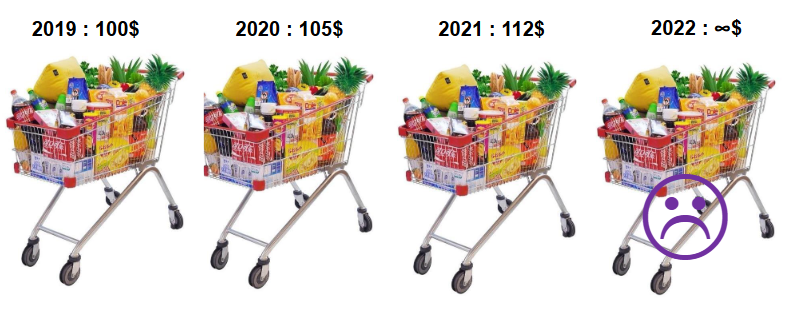
\includegraphics[width=0.7\textwidth]{assets/inflatie.png}
    \caption{Effect van inflatie op koopkracht}
    \label{fig:inflatie}
\end{figure}
\FloatBarrier

Inflatie wordt berekend met de formule:
\frm{Inflatie formule}{
    K = k(1 + i)^n
}
{met $K$ de toekomstige waarde, $k$ de huidige waarde,
    $i$ het inflatiepercentage en $n$ de hoeveelheid periodes.}

\begin{oefenblok}[Voorbeeldoefening: Koopkracht over tijd]
    Stel dat je vandaag \text{€}1.000 op je spaarrekening hebt. De gemiddelde inflatie over de komende 5 jaar wordt geschat op 3\% per jaar. Hoeveel moet dat bedrag over 5 jaar zijn om nog exact dezelfde hoeveelheid goederen te kunnen kopen?

    \textbf{Oplossing:}
    \begin{itemize}
        \item \textbf{Gegeven:} $k = \text{€}1.000$, $i = 0,03$ (3\%), $n = 5$ jaar.
        \item \textbf{Berekening:}
              \[ K = 1000 \times (1 + 0,03)^5 \]
              \[ K = 1000 \times (1,03)^5 \approx 1000 \times 1,159 \]
        \item \textbf{Resultaat:} $K = \mathbf{\text{€}1.159,27}$
    \end{itemize}
    \textit{Betekenis:} Door de inflatie heb je over 5 jaar \text{€}1.159,27 nodig om hetzelfde te kunnen kopen als wat je vandaag voor \text{€}1.000 koopt. Je geld is dus minder waard geworden.
\end{oefenblok}


\subsection{Basisgegevens investeringsevaluatie}
Een paar belangrijke begrippen bij investeringsevaluatie:
\begin{description}
    \item[Horizon] De periode waarin je de investering bekijkt (bijv. 5 jaar).
          \begin{itemize}
              \item fysieke levensduur: Hoe lang gaat de investering mee?
              \item economische levensduur: Hoe lang levert de investering waarde op?
              \item Fiscale levensduur: Hoe lang mag je de investering afschrijven volgens de belastingdienst?
              \item Product levensduur: Hoe lang blijft het product relevant op de markt? zie module 1.
          \end{itemize}
    \item[Uitgavepatroon] Wanneer worden de kosten gemaakt?
    \item[Inkomstenpatroon] Wanneer worden de opbrengsten gegenereerd?
\end{description}

\begin{figure}[ht]
    \centering
    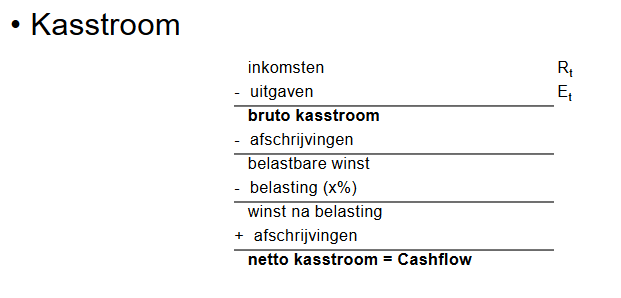
\includegraphics[width=0.7\textwidth]{assets/Kasstroom.png}
    \caption{Uitgave- en inkomstenpatroon van een investering}
    \label{fig:investeerpatroon}
\end{figure}

\subsection{Afschrijvingen}

\begin{conceptbox}

    Een \concept{afschrijving} is een manier om de kosten van een investering te verdelen over de
    meerdere periodes. Dit is belangrijk voor de belastingen.
    Je kunt namelijk belastingen vermijden door afschrijvingen te gebruiken.
    \newline
\end{conceptbox}

Stel: je hebt 6.500 euro inkomsten en 500 euro uitgaven.
De bruto cashflow is dan 6.000 euro. Je doet nu een investering: een fiets van 5.000 euro,
die je over 5 jaar afschrijft. Elk jaar schrijf je dus 1.000 euro af.
De belastbare basis wordt dan $6.000 - 1.000 = 5.000$ euro.
De belastingen zijn 20\%, dus je betaalt 1.000 euro belasting en houdt 4.000 euro over.
Daarna tel je de afschrijving er weer bij, omdat het geen echte uitgave van dit jaar is:
je netto cashflow is $4.000 + 1.000 = 5.000$ euro.
Zonder afschrijving had je $6.000 \times 0{,}8 = 4.800$ euro overgehouden;
de afschrijving levert je dus 200 euro belastingvoordeel op.
\newline

Waarom werkt dat zo? Je hebt de fiets in één keer uit je portemonnee betaald,
maar het is een investering voor de lange termijn. Zo'n investering mag je over
meerdere periodes spreiden. Elke periode leg je een stuk van de aankoopprijs als kost
in je boeken, terwijl er die periode geen geld meer wegvloeit.
Dat is een afschrijving: ze verlaagt je belastbare winst zonder dat je opnieuw betaalt.
\newline

Een afschrijving mag niet altijd. Je mag niet zomaar 100\% van je aankoop in één keer afschrijven.
Je moet dus, afhankelijk van je product, een afschrijvingstermijn en een afschrijvingsmethode kiezen.
\newline

\belangrijk{De fiscus} is de belastingdienst die belastingen heft.
Zij bepalen dus hoe lang en op welke manier je mag afschrijven.
\newline

Je hebt verschillende manieren van afschrijven:

\noindent\textbf{Lineaire afschrijving:} Elk jaar hetzelfde bedrag zoals het voorbeeld hierboven.\\
\begin{minipage}[t]{0.58\textwidth}
    \vspace{0pt}
    \begin{itemize}
        \item \textbf{Voordelen:} Wordt aanvaard door de fiscus en is eenvoudig te berekenen.
        \item \textbf{Nadelen:} Je schrijft altijd een vast bedrag af, ongeacht het gebruik of de waarde van het actief.
    \end{itemize}
\end{minipage}%
\hfill
\begin{minipage}[t]{0.4\textwidth}
    \vspace{0pt}
    \centering
    \begin{tikzpicture}
        \begin{axis}[
                ybar,
                width=\linewidth,
                height=3.4cm,
                ylabel={Afschrijving},
                xlabel={Periode},
                xtick=data,
                ymin=0,
                ymax=28,
                bar width=9pt,
                nodes near coords,
                every node near coord/.append style={font=\scriptsize},
                ylabel style={font=\scriptsize},
                xlabel style={font=\scriptsize},
                tick label style={font=\scriptsize},
                axis lines=left,
                enlarge x limits=0.14,
                ymajorgrids, grid style={gray!25}
            ]
            \addplot[fill=schoolBlue!70, draw=black!55] coordinates {(1,20) (2,20) (3,20) (4,20) (5,20)};
        \end{axis}
    \end{tikzpicture}
\end{minipage}

\vspace{0.5em}
\noindent\textbf{Degressieve afschrijving:} Meer afschrijven in het begin en minder later.\\
\begin{minipage}[t]{0.58\textwidth}
    \vspace{0pt}
    \begin{itemize}
        \item \textbf{Voordelen:} Je schrijft meer af in het begin, waardoor je vroeg minder belasting betaalt.
        \item \textbf{Nadelen:} Soms niet aanvaard door de fiscus.
    \end{itemize}
\end{minipage}%
\hfill
\begin{minipage}[t]{0.4\textwidth}
    \vspace{0pt}
    \centering
    \begin{tikzpicture}
        \begin{axis}[
                ybar,
                width=\linewidth,
                height=3.4cm,
                ylabel={Afschrijving},
                xlabel={Periode},
                xtick=data,
                ymin=0,
                ymax=50,
                bar width=9pt,
                nodes near coords,
                every node near coord/.append style={font=\scriptsize},
                ylabel style={font=\scriptsize},
                xlabel style={font=\scriptsize},
                tick label style={font=\scriptsize},
                axis lines=left,
                enlarge x limits=0.14,
                ymajorgrids, grid style={gray!25}
            ]
            \addplot[fill=schoolRed!70, draw=black!55] coordinates {(1,40) (2,30) (3,20) (4,13) (5,7)};
        \end{axis}
    \end{tikzpicture}
\end{minipage}

\vspace{0.5em}
\noindent\textbf{Vertraagde afschrijving:} Minder afschrijven in het begin en meer later.\\
\begin{minipage}[t]{0.58\textwidth}
    \vspace{0pt}
    \begin{itemize}
        \item \textbf{Voordelen:} De fiscus gaat dit altijd aanvaarden.
        \item \textbf{Nadelen:} Fiscaal niet interessant, omdat je in het begin méér belasting betaalt.
    \end{itemize}
\end{minipage}%
\hfill
\begin{minipage}[t]{0.4\textwidth}
    \vspace{0pt}
    \centering
    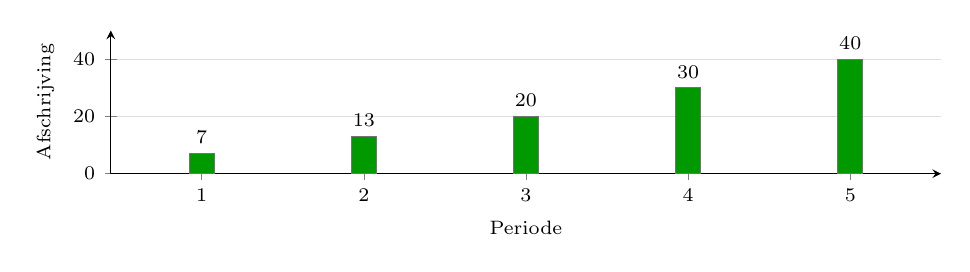
\begin{tikzpicture}
        \begin{axis}[
                ybar,
                width=\linewidth,
                height=3.4cm,
                ylabel={Afschrijving},
                xlabel={Periode},
                xtick=data,
                ymin=0,
                ymax=50,
                bar width=9pt,
                nodes near coords,
                every node near coord/.append style={font=\scriptsize},
                ylabel style={font=\scriptsize},
                xlabel style={font=\scriptsize},
                tick label style={font=\scriptsize},
                axis lines=left,
                enlarge x limits=0.14,
                ymajorgrids, grid style={gray!25}
            ]
            \addplot[fill=green!60!black, draw=black!55] coordinates {(1,7) (2,13) (3,20) (4,30) (5,40)};
        \end{axis}
    \end{tikzpicture}
\end{minipage}

\vspace{0.5em}
\vspace{0.5em}
\noindent\textbf{Reële waarde-afschrijving:} Je schrijft af naar werkelijk gebruik
\textit{(hoeveel kilometer heeft de vrachtwagen dit jaar gereden?)}.\\
\begin{minipage}[t]{0.58\textwidth}
    \vspace{0pt}
    \begin{itemize}
        \item \textbf{Voordelen:} Je schrijft af afhankelijk van het gebruik.
        \item \textbf{Nadelen:} Moeilijk te berekenen maar klopt met de realiteit.
    \end{itemize}
\end{minipage}%
\hfill
\begin{minipage}[t]{0.4\textwidth}
    \vspace{0pt}
    \centering
    \begin{tikzpicture}
        \begin{axis}[
                ybar,
                width=\linewidth,
                height=3.4cm,
                ylabel={Afschrijving},
                xlabel={Periode},
                xtick=data,
                ymin=0,
                ymax=40,
                bar width=9pt,
                nodes near coords,
                every node near coord/.append style={font=\scriptsize},
                ylabel style={font=\scriptsize},
                xlabel style={font=\scriptsize},
                tick label style={font=\scriptsize},
                axis lines=left,
                enlarge x limits=0.14,
                ymajorgrids, grid style={gray!25}
            ]
            \addplot[fill=schoolOrange!80, draw=black!55] coordinates {(1,15) (2,30) (3,25) (4,18) (5,10)};
        \end{axis}
    \end{tikzpicture}
\end{minipage}

In het begin meer afschrijven is fiscaal voordeliger, omdat je dan vroeger minder belasting betaalt,
maar de fiscus laat dit niet altijd toe.

\begin{examenbox}
    Zorg dat je weet wat afschrijvingen zijn en de verschillende soorten afschrijvingen kent en de Voordelen
    en Nadelen ervan.
\end{examenbox}

\subsection{Wat mag je nu afschrijven?}
In de slides staat er een ijsberg
met wat je mag afschrijven. Hoe dieper
hoe langer het duurt om af te schrijven.
Je mag dingen afschrijven als ze economisch nuttig zijn en
tot de activa (dingen die in het bezit van het bedrijf behoren).
Je mag bijvoorbeeld geen computer afschrijven
als die niet voor het bedrijf gebruikt wordt.
Onderhoud en operationele kosten schrijf je niet af: die boek je meteen als kost
in het jaar zelf. Alleen de aankoopkosten van het actief zelf worden afgeschreven.


\begin{figure}[ht]
    \centering
    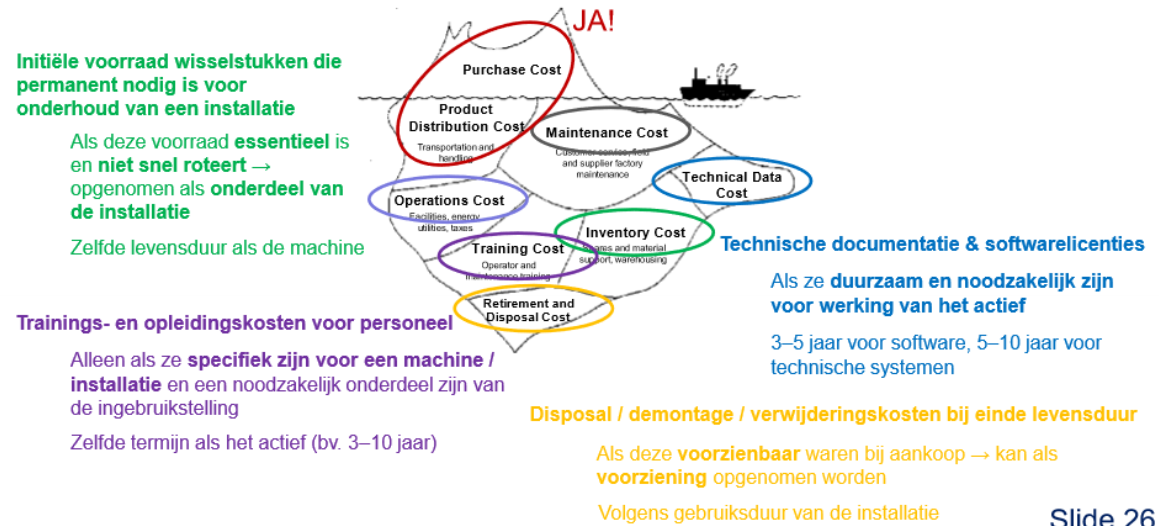
\includegraphics[width=1\textwidth]{assets/AfschrijfLimiet.png}
    \caption{Wat mag je afschrijven}
    \label{fig:AfschrijfLimiet.png}
\end{figure}
\FloatBarrier


\subsection{Samengestelde interest, actualisatie, en annuïteiten}

\noindent\textbf{Compound interest:}\\
\begin{minipage}[t]{0.45\textwidth}
    \vspace{0pt}
    Interest die wordt verdiend op zowel het oorspronkelijke bedrag als op de eerder verdiende interest.
    Je krijgt dus een "rente op rente" effect. Dit leidt tot exponentiële groei van investeringen over tijd.
\end{minipage}%
\hfill
\begin{minipage}[t]{0.5\textwidth}
    \vspace{0pt}
    \centering
    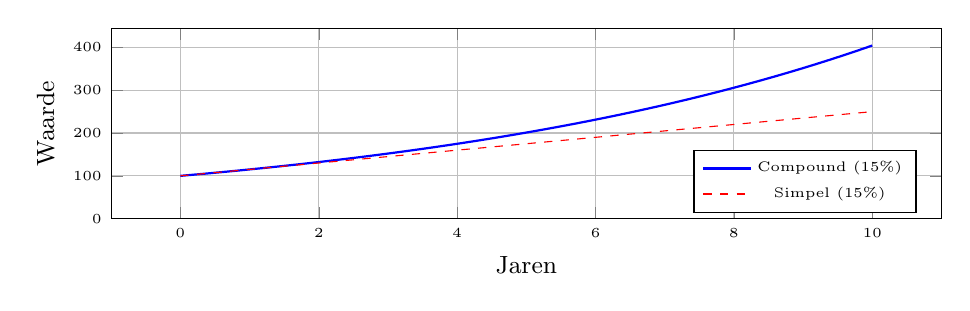
\begin{tikzpicture}
        \begin{axis}[
                width=\textwidth,
                height=4cm,
                xlabel={Jaren},
                ylabel={Waarde},
                grid=major,
                ymin=0,
                ylabel style={font=\small},
                xlabel style={font=\small},
                tick label style={font=\tiny},
                legend pos=south east,
                legend style={font=\tiny}
            ]
            \addplot[blue, thick, domain=0:10, samples=50] {100*(1.15)^x};
            \addlegendentry{Compound (15\%)}
            \addplot[red, dashed, domain=0:10] {100 + 15*x};
            \addlegendentry{Simpel (15\%)}
        \end{axis}
    \end{tikzpicture}
\end{minipage}

\vspace{0.5em}
\noindent\textbf{Opportunity cost:}\\
\begin{minipage}[t]{0.45\textwidth}
    \vspace{0pt}
    De potentiële opbrengst die je misloopt door te kiezen voor een bepaalde investering in plaats van de beste alternatieve investering.
    Deze is te berekenen met de formule van inflatie, maar dan met een positief rentepercentage.
\end{minipage}%
\hfill
\begin{minipage}[t]{0.5\textwidth}
    \vspace{0pt}
    \centering
    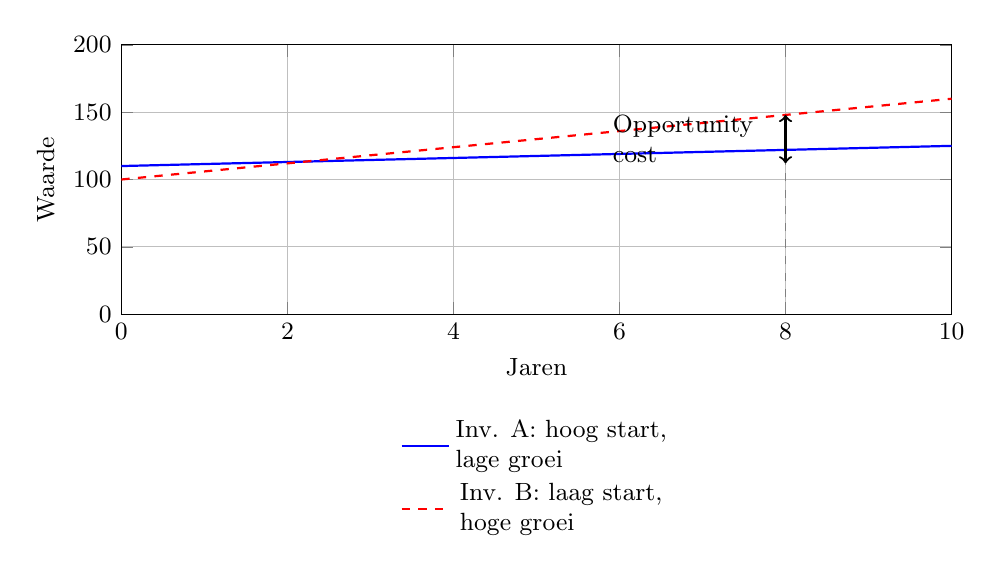
\begin{tikzpicture}
        \begin{axis}[
                xlabel=Jaren,
                ylabel=Waarde,
                xmin=0, xmax=10,
                ymin=0, ymax=200,
                xtick={0, 2, 4, 6, 8, 10},
                ytick={0, 50, 100, 150, 200},
                grid=major,
                legend style={
                        at={(0.5,-0.35)},
                        anchor=north,
                        legend columns=1,
                        draw=none,
                        font=\small,
                        align=left
                    },
                width=\textwidth, height=5cm,
                ylabel style={font=\small},
                xlabel style={font=\small},
                tick label style={font=\small}
            ]

            % Investering A (hoog startbedrag, lage groei)
            \addplot[blue, thick, domain=0:10, samples=20] {110 + 1.5*x};
            \addlegendentry{Inv. A: hoog start,\\ lage groei};

            % Investering B (laag startbedrag, hoge groei)
            \addplot[red, dashed, thick, domain=0:10, samples=20] {100 + 6*x};
            \addlegendentry{Inv. B: laag start,\\ hoge groei};

            % Opportunity Cost Annotation at Year 8 (outside graph)
            \draw[dashed, gray] (axis cs:8,0) -- (axis cs:8,148);
            \draw[<->, thick, black] (axis cs:8,112) -- (axis cs:8,148)
            node[midway, left=8pt, font=\small, align=left] {Opportunity\\ cost};

        \end{axis}
    \end{tikzpicture}
\end{minipage}

\begin{oefenblok}
    Stel dat je vandaag €2.000 investeert in een spaarrekening met een samengestelde jaarlijkse rente van 4\%. Hoeveel geld heb je na 6 jaar?

    \textbf{Oplossing:}
    \begin{itemize}
        \item \textbf{Gegeven:} $P = €2.000$, $i = 0,04$ (4\%), $n = 6$ jaar.
        \item \textbf{Berekening:}
              \[ F = 2000 \times (1 + 0,04)^6 \]
              \[ F = 2000 \times (1,04)^6 \approx 2000 \times 1,265319 \]
        \item \textbf{Resultaat:} $F = \mathbf{€2.530,64}$
    \end{itemize}
\end{oefenblok}

\begin{oefenblok}
    Je hebt de keuze tussen twee investeringen:
    \begin{itemize}
        \item Investering A: Een obligatie die na 3 jaar €1.500 oplevert.
        \item Investering B: Een spaarrekening met een samengestelde jaarlijkse rente van 5\%.
        \item Je hebt €1.200 beschikbaar om te investeren.
    \end{itemize}

    \textbf{Vraag:} Wat is de opportunity cost van het kiezen voor Investering A in plaats van Investering B?

    \textbf{Oplossing:}
    \begin{itemize}
        \item \textbf{Berekening van Investering B:}
              \[ F_B = 1200 \times (1 + 0,05)^3 \]
              \[ F_B = 1200 \times (1,05)^3 \approx 1200 \times 1,157625 \]
              \[ F_B \approx €1.389,15 \]
        \item \textbf{Opportunity cost van A:} dat is wat je misloopt door B \emph{niet} te kiezen:
              \[ \text{Opportunity cost} = F_B = €1.389,15 \]
        \item \textbf{Vergelijking:} A levert €1.500 op, B slechts €1.389,15.
              \[ 1500 - 1389,15 = €110,85 \text{ voordeel voor A} \]
              De opbrengst van A ligt hoger dan de opportunity cost, dus A is de betere keuze.
    \end{itemize}
\end{oefenblok}

\subsection{Actualisatie en annuïteiten}

Hoe kunnen we nu weten wat de waarde is van toekomstige cashflows in het heden?
Of als we iets afbetalen in termijnen, wat is dan de waarde van die betalingen nu?
Dus je brengt toekomstige cashflows (A) terug naar hun huidige waarde (P).
Dit proces noemen we \textbf{actualisatie}.

Laten we eerst een simpel voorbeeld bekijken.
\frm{Formule huidige waarde (actualisatie van één bedrag)}
{P = \frac{F}{(1 + i)^n}}
{met $P$ de huidige waarde, $F$ de toekomstige waarde, $i$ de rentevoet en $n$ het aantal periodes.}

Stel ik wil over 5 jaar 1000 euro ontvangen. De rentevoet is 5\%.
Wat moet ik investeren nu om dat bedrag te krijgen?
\[
    P = \frac{1000}{(1 + 0{,}05)^5} = 783{,}53~\text{€}
\]
Dus als ik nu 783,53 euro investeer tegen 5\% rente, dan heb ik over 5 jaar 1.000 euro.
\newline

\begin{figure}[ht]
    \centering
    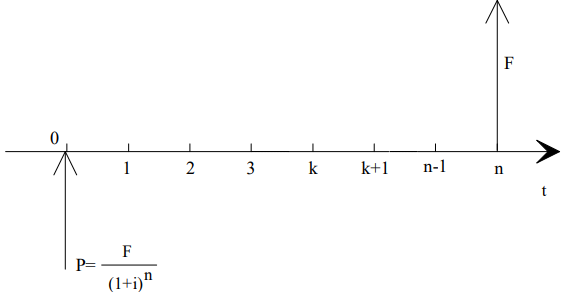
\includegraphics[width=0.7\textwidth]{assets/image1.png}
    \caption{Actualisatie van één toekomstig bedrag}
    \label{fig:toekomstigewaarde}
\end{figure}
\FloatBarrier
Dit is natuurlijk simpel. Het gaat over 1 bedrag in de toekomst.
Wat als we nu een reeks van bedragen hebben?


\subsubsection{Actualisatie}
\belangrijk{Actualisatie} is het proces van het omzetten van toekomstige cashflows naar hun huidige waarde.
Door inflatie wordt dit geld minder waard in de toekomst. Je wilt dus weten
als ik in de toekomst geld krijg, hoeveel is dat nu waard?
\begin{figure}[ht]
    \centering
    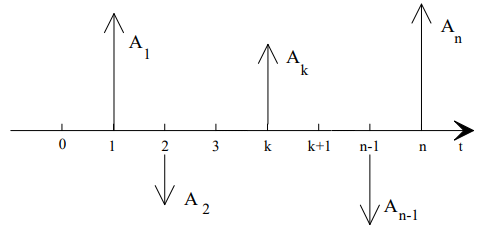
\includegraphics[width=0.7\textwidth]{assets/image2.png}
    \caption{Actualisatie van toekomstige cashflows}
    \label{fig:actualisatie}
\end{figure}
\FloatBarrier

De formule voor actualisatie is:

\frm{Formule actualisatie}{
    P = \frac{A_1}{(1 + i)^1} + \frac{A_2}{(1 + i)^2} + \cdots + \frac{A_n}{(1 + i)^n} =
    \sum_{k=1}^{n} \frac{A_k}{(1 + i)^k}
}
{met $P$ de huidige waarde, $A_k$ de cashflow in periode $k$, $i$ de rentevoet en $n$ het aantal periodes.}

Laten we een voorbeeld bekijken.
Stel je hebt de volgende cashflows over 3 jaar:
\begin{itemize}
    \item Jaar 1: 1000 euro
    \item Jaar 2: 1500 euro
    \item Jaar 3: 2000 euro
    \item Rentevoet i = 5\%
\end{itemize}
De huidige waarde van deze cashflows is:
\[
    \begin{aligned}
        P & = \frac{1000}{(1 + 0.05)^1} + \frac{1500}{(1 + 0.05)^2} + \frac{2000}{(1 + 0.05)^3} \\
          & = \frac{1000}{1.05} + \frac{1500}{1.1025} + \frac{2000}{1.157625}                   \\
          & \approx 952{,}38 + 1360{,}54 + 1727{,}68 = 4040{,}60~\text{€}
    \end{aligned}
\]

Dus met deze toekomstige cashflows heb je nu een waarde van ongeveer 4.040,60 euro.
\newline

Dit zijn alleen cashflows die je ontvangt. Wat als je een lening hebt die je moet afbetalen in termijnen?
Dit noemen we een annuïteit.
\newline
\subsubsection{Annuïteiten}
\belangrijk{Annuïteit} is een reeks gelijke betalingen die op regelmatige tijdstippen worden gedaan.
Als je een lening aangaat bij de bank, dan betaal je meestal in maandelijkse termijnen.
Je terugbetaling A is dan constant. Hoe bereken je die A?
\newline

De formule voor de huidige waarde van een annuïteit is:
\frm{Formule annuïteit}{
    P = A \sum_{k=1}^{n} \frac{1}{(1 + i)^k} = A \left( \frac{1 - (1 + i)^{-n}}{i} \right) = A \times a_n
}
{met $P$ de huidige waarde (het geleende bedrag), $A$ de annuïteit (termijnbetaling), $i$ de rentevoet,
    $a_n$ de annuïteitsfactor en $n$ het aantal periodes.}
Laten we een voorbeeld bekijken.
Stel je leent 500 euro bij de bank tegen een rentevoet van 10\% per jaar.
Je wilt dit terugbetalen in 10 jaarlijkse termijnen. Wat is de jaarlijkse betaling A?
Weet dat A hoger zal zijn want je moet ook rente betalen.
\[
    500 = A \left( \frac{1 - (1 + 0.10)^{-10}}{0.10} \right)
\]
\[
    \begin{aligned}
        500 & = A \left( \frac{1 - (1{,}10)^{-10}}{0{,}10} \right)
        = A \left( \frac{1 - 0{,}38554}{0{,}10} \right)
        = A \left( \frac{0{,}61446}{0{,}10} \right) = A \times 6{,}1446 \\[4pt]
        A   & = \frac{500}{6{,}1446} \approx 81{,}37~\text{€}
    \end{aligned}
\]

6,1446 is de \belangrijk{annuïteitsfactor} $a_{10}$. Je kunt die berekenen of opzoeken in een tabel:
je zoekt dan 10 jaar en 10\% op.
Dus je moet elk jaar 81,37 euro betalen om de lening van 500 euro in 10 jaar terug te betalen.
\newline

Zetten we dit in een tabel, dan zie je duidelijk wat je elk jaar afbetaalt.
\begin{table}[H]
    \centering
    \caption{Afbetalingsschema van de lening}
    \begin{tabular}{r r r r r r}
        \toprule
        Periode & Beginbalans (€) & Rente (10\%)         & Betaling (€) & Aflossing (€) & Eindbalans (€) \\
        \midrule
        1       & 500,00          & $500 \times 0{,}10 = 50{,}00$ & 81,37        & 31,37         & 468,63         \\
        2       & 468,63          & 46,86                         & 81,37        & 34,51         & 434,12         \\
        3       & 434,12          & 43,41                         & 81,37        & 37,96         & 396,17         \\
        4       & 396,17          & 39,62                         & 81,37        & 41,75         & 354,41         \\
        5       & 354,41          & 35,44                         & 81,37        & 45,93         & 308,48         \\
        6       & 308,48          & 30,85                         & 81,37        & 50,52         & 257,96         \\
        7       & 257,96          & 25,80                         & 81,37        & 55,57         & 202,39         \\
        8       & 202,39          & 20,24                         & 81,37        & 61,13         & 141,26         \\
        9       & 141,26          & 14,13                         & 81,37        & 67,24         & 74,01          \\
        10      & 74,01           & 7,40                          & 81,41        & 74,01         & 0,00           \\
        \bottomrule
    \end{tabular}
\end{table}

Opmerking: de vaste periodieke betaling is $A \approx$ €81,37; de laatste betaling is hier licht
aangepast (€81,41) om de afrondingsverschillen weg te werken.

Je betaalt dus steeds minder interest, omdat je schuld afneemt.
\newline


\subsection{Investeringsevaluatie methodes}
Hoe weten we nu of een investering goed is of niet?
Deze formules geven ons een manier om dat te bepalen.
We gaan hier twee methodes bekijken.

\subsubsection{Payback-methode}

\noindent
\begin{minipage}{0.55\textwidth}
    De payback-methode kijkt naar hoe snel je je investering terugverdient.
    Dit is een simpele methode die niet kijkt naar de tijdswaarde van geld.
    Je berekent gewoon hoeveel tijd het duurt om je initiële investering terug te krijgen.
    Het is mogelijk dat je hierdoor winst mist omdat je niet kijkt naar de cashflows na de payback-periode.
\end{minipage}\hfill
\begin{minipage}{0.4\textwidth}
    \centering
    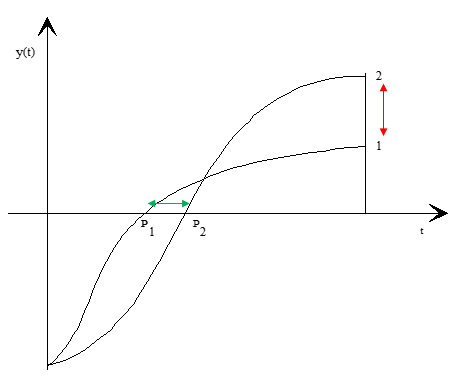
\includegraphics[width=\linewidth]{assets/Paypackperiode.png}\\[4pt]
    {\small\textbf{Payback-periode illustratie}\label{fig:Paypackperiode}}
\end{minipage}

\begin{itemize}
    \item \textbf{Voordelen:} Eenvoudig te begrijpen en toe te passen. Handig voor snelle beslissingen.
    \item \textbf{Nadelen:} Negeert de tijdswaarde van geld en cashflows na de payback-periode.
    \item \textbf{Toepassing:} Geschikt voor kleine investeringen of wanneer liquiditeit belangrijk is.
\end{itemize}

\subsubsection{Discounted cashflow}
De discounted cashflow (DCF) methode houdt rekening met de tijdswaarde van geld.
Als het over lange termijn investeringen gaat, is dit de beste methode.

\frm{Formule Huidige Waarde (HW)}
{
    HW = \sum_{k=0}^{n} \frac{R_k-E_k}{(1 + i)^k} = \sum_{k=0}^{n} \frac{CF_k}{(1 + i)^k}
}
{met $HW$ de huidige waarde, $R_k$ de inkomsten in periode $k$, $E_k$ de uitgaven in periode $k$, $i$ de discontovoet, $CF_k$ de cashflow in periode $k$, en $n$ de hoeveelheid periodes.}
De netto huidige waarde (NHW) is dan:
\frm{Formule Netto Huidige Waarde (NHW)}
{
    NHW = HW - I_0 = \sum_{k=0}^{n} \frac{CF_k}{(1 + i)^k} - I_0
}
{met $NHW$ de netto huidige waarde, $HW$ de huidige waarde, $I_0$ de initiële investering, $CF_k$ de cashflow in periode
    $k$, $i$ de discontovoet, en $n$ de hoeveelheid periodes.}

Als NHW > 0, is de investering rendabel.
\newline

Hiermee kunnen we de Profitability Index (PI) berekenen:
\frm{Formule Profitability Index (PI)}
{
    PI_1 = \frac{HW}{I_0} \qquad PI_2 = \frac{NHW}{I_0} = PI_1 - 1
}
{met $PI_1$ de profitability index t.o.v.\ de huidige waarde, $PI_2$ dezelfde index t.o.v.\ de netto huidige waarde,
    $NHW$ de netto huidige waarde, $HW$ de huidige waarde en $I_0$ de initiële investering.}

Je hebt dus een factor die zegt hoeveel je per geïnvesteerde euro terugkrijgt.
Is $PI_1 > 1$ (en dus $PI_2 > 0$), dan is de investering goed.
\newline

Als laatste hebben we de Internal Rate of Return (IRR).
In de formule \ref{frm:6} van NHW, stel je NHW = 0.
Je lost dan op voor i. Dit is de IRR.
Dit toont hoeveel rendement je krijgt op je investering.
\frm{Formule Internal Rate of Return (IRR)}
{
    0 = \sum_{k=0}^{n} \frac{CF_k}{(1 + IRR)^k} - I_0
}
{met $IRR$ de internal rate of return,
    $CF_k$ de cashflow in periode $k$, $I_0$ de initiële investering, en $n$ de hoeveelheid periodes.}

\begin{figure}[ht]
    \centering
    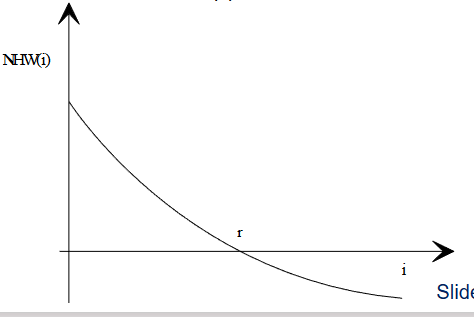
\includegraphics[width=0.5\textwidth]{assets/rateofreturn.png}
    \caption{Grafische weergave van de IRR (snijpunt met de x-as)}
    \label{fig:rateofreturn.png}
\end{figure}
\FloatBarrier



\begin{examenbox}
    De formules zijn gegeven maar weet wat ze betekenen en hoe je ze gebruikt.
    Zorg ook dat je de voordelen en nadelen van de twee methodes kent.
    Je hebt twee methodes: Payback en Discounted Cashflow.
    Payback is simpel maar kijkt niet naar de tijdswaarde van geld.
    Discounted Cashflow is complexer maar geeft een beter beeld van de investering over tijd.
\end{examenbox}

\begin{oefenblok}[IRR Berekening]
    \textbf{Opgave:} Je bedrijf overweegt een investering van €50.000.
    De cashflows voor de komende 4 jaar zijn respectievelijk:
    \begin{itemize}
        \item Jaar 0: -€50.000 (initiële investering)
        \item Jaar 1: €15.000
        \item Jaar 2: €18.000
        \item Jaar 3: €16.000
        \item Jaar 4: €14.000
    \end{itemize}

    \textbf{Bepaal de IRR van deze investering.}

    \vspace{5mm}

    \textbf{Oplossing:}

    We gebruiken de IRR-formule:
    $$0 = -50.000 + \frac{15.000}{(1+IRR)^1} + \frac{18.000}{(1+IRR)^2} + \frac{16.000}{(1+IRR)^3} + \frac{14.000}{(1+IRR)^4}$$

    Dit is een niet-lineaire vergelijking die we niet analytisch kunnen oplossen.
    We gebruiken \textbf{iteratie} of een \textbf{financiële calculator}:

    \begin{itemize}
        \item Bij $IRR = 0\%$: NHW $= 15.000 + 18.000 + 16.000 + 14.000 - 50.000 = +€13.000$
        \item Bij $IRR = 10\%$: NHW $= \frac{15.000}{1,10} + \frac{18.000}{1,21} + \frac{16.000}{1,331} + \frac{14.000}{1,4641} - 50.000$ \\
              $= 13.636,36 + 14.876,03 + 12.021,04 + 9.562,19 - 50.000 \approx +€95,62$
        \item Bij $IRR = 11\%$: NHW $\approx -€956$
    \end{itemize}

    De NHW wisselt van teken tussen 10\% en 11\%, dus daar ligt de IRR. Lineaire interpolatie:
    \[
        IRR \approx 0{,}10 + \frac{95{,}62}{95{,}62 + 956} \times (0{,}11 - 0{,}10) \approx \mathbf{10{,}1\%}
    \]

    \textbf{Conclusie:} De investering levert ongeveer 10,1\% rendement op.
    Als dit hoger is dan de geëiste rentabiliteit (hurdle rate), accepteer je de investering.
\end{oefenblok}



\begin{oefenblok}[Oefening: Discounted Cashflow — HW, NHW, IRR, PI]
    Gegeven: initiële investering $I_0=\text{€}5.000$. Verwachte cashflows:
    \[
        CF_1=\text{€}1.500,\quad CF_2=\text{€}2.000,\quad CF_3=\text{€}2.500.
    \]
    Discontovoet $i=8\%$.

    \textbf{1. Huidige Waarde (HW)}\\
    $HW=\sum_{k=1}^{n}\frac{CF_k}{(1+i)^k}$
    Berekening:
    \[
        \begin{aligned}
            HW & = \frac{1500}{1{,}08}+\frac{2000}{1{,}08^2}+\frac{2500}{1{,}08^3}         \\
               & \approx 1388{,}89 + 1714{,}68 + 1984{,}58 = \mathbf{5088{,}15\ \text{€}}.
        \end{aligned}
    \]

    \textbf{2. Netto Huidige Waarde (NHW)}\\
    $NHW = HW - I_0$
    \[
        NHW = 5088{,}15 - 5000 = \mathbf{88{,}15\ \text{€}} \quad (>0 \Rightarrow \text{rendabel bij }8\%).
    \]

    \textbf{3. Profitability Index (PI)}\\
    $PI = \frac{HW}{I_0}$
    \[
        PI = \frac{5088{,}15}{5000} \approx \mathbf{1{,}0176}.
    \]
    \textbf{4. Internal Rate of Return (IRR)}\\
    IRR is de koers $r$ waarvoor
    \[
        0 = \left(\sum_{k=1}^{3}\frac{CF_k}{(1+r)^k}\right) - I_0.
    \]
    We zoeken $r$ door iteratie. De NHW bij $r=8\%$ is $+88{,}15$, bij $r=9\%$ is ongeveer $-10{,}03$. Lineaire interpolatie geeft:
    \[
        r \approx 0{,}08 + \frac{88{,}15}{88{,}15 + 10{,}03}\times(0{,}09-0{,}08)
        \approx \mathbf{8{,}90\%}.
    \]
    \textbf{Conclusie:} HW = €5.088,15, NHW = €88,15 ($>0$), PI $\approx$ 1,018, IRR $\approx$ 8,90\%. Het project is rendabel bij een discontovoet van 8\%.
\end{oefenblok}

\begin{examenbox}
    Een vraag kan zijn: \textit{``Hoe voer je een investeringsanalyse uit? Leg uit aan de hand van een schema.''}
    Je legt uit welke waarden je allemaal nodig hebt en hoe je die berekent (cashflow, intrest, investeringperiode, het investeringsbedrag, etc).
    Daarna leg je uit welke methodes er zijn (NHW, IRR \dots) en hoe je die berekent.
    Leg dan wanneer het een goede of slechte investering is voor welke voorwaarden.
\end{examenbox}

\begin{examenbox}
    \textit{``Stel je wilt een investering analyseren die een effect zou hebben over een periode van 10 jaar.
        Welke beoordelingscriteria zou je gebruiken, en waarom? Motiveer duidelijk je antwoord.''}
    Je gebruikt sowieso discounted cashflow, omdat je met een periode van 10 jaar werkt: over zo'n horizon
    weegt de tijdswaarde van geld zwaar door. Voor kleine, kortlopende investeringen volstaat payback.
\end{examenbox}

\begin{examenbox}
    \textit{``Investeringen en subsidies. Hoe kunnen subsidies bepalend zijn bij een investeringsevaluatie? Leg uit.''}
    Als je investering gesubsidieerd wordt, verlaagt dat het initiële investeringsbedrag $I_0$.
    In de formules van NHW en IRR zit $I_0$ als negatieve term, dus een lagere $I_0$ verhoogt de NHW
    en de IRR: een project dat zonder subsidie afgekeurd wordt, kan mét subsidie wel rendabel zijn.
\end{examenbox}


\section{Module 4: Kostprijs calculatie}

Dit deel gaat over kostprijs calculatie. Je gaat dus berekenen wat de kost is van een product.
Dit is niet hetzelfde als de prijszetting. Hierbij bekijk je puur wat het kost om een product te maken.
We willen dus weten wat de kost is van grondstoffen, arbeid, overhead, etc.
Daarna kan je met deze factoren de prijs bepalen.
\newline

We nemen een pizzeria als voorbeeld.
Die heeft kosten voor ingrediënten, de kok, huur, elektriciteit, management enzovoort.

\subsection{Kostprijs elementen}


\begin{table}[ht]
    \centering
    \begin{tabular}{c|c|c}
        \textbf{Kostentype}                                                                                                 & \textbf{Variabele Kosten} & \textbf{Vaste Kosten} \\
        \hline
        \textbf{Directe Kosten}                                                                                             &
        \begin{tabular}[t]{@{}l@{}}Grondstof per eenheid \\ Arbeid per eenheid \\ Directe materiaal\end{tabular}            &
        \begin{tabular}[t]{@{}l@{}}Vaste arbeid \\ Gespecialiseerde machines \\ Licenties specifiek product\end{tabular}                                                        \\
        \hline
        \textbf{Indirecte Kosten}                                                                                           &
        \begin{tabular}[t]{@{}l@{}}Energie voor productie \\ Distributie per eenheid \\ Verpakking per eenheid\end{tabular} &
        \begin{tabular}[t]{@{}l@{}}Administratie \\ Huur fabriek \\ Verzekeringen \\ Onderhoud machines\end{tabular}                                                            \\
        \hline
    \end{tabular}
    \caption{Kostenmatrix: Categorisering naar Directheid en Variabiliteit}
    \label{tab:kostenmatrix}
\end{table}

\begin{conceptbox}[Kostprijs elementen]

    \begin{itemize}
        \item \textbf{Variabele kosten:} Veranderen met de hoeveelheid geproduceerde eenheden \textit{(ingrediënten per pizza)}.
        \item \textbf{Vaste kosten:} Blijven hetzelfde, onafhankelijk van de productie \textit{(huur, salarissen administratie)}.
        \item \textbf{Directe kosten:} Rechtstreeks toewijsbaar aan een product of dienst \textit{(deeg per pizza)}.
        \item \textbf{Indirecte kosten:} Niet rechtstreeks toewijsbaar aan één product \textit{(elektriciteit van de pizzeria, huur van het gebouw)}.
    \end{itemize}
\end{conceptbox}

Indirecte kosten hangen dus niet aan één product, maar ze horen wel bij de kostprijs.
Je moet ze dus via een verdeelsleutel toch aan de producten toewijzen.
\newline

Voorbeelden:
Het deeg is een \textbf{variabele directe} kost: gelinkt aan het product en meestijgend met de productie.
De huur is een \textbf{vaste indirecte} kost: niet gelinkt aan één product en niet afhankelijk van de productie.
Elektriciteit is een \textbf{variabele indirecte} kost: niet gelinkt aan één product, maar wel meestijgend met de productie.
De kok is een \textbf{vaste directe} kost: gelinkt aan het product, maar niet afhankelijk van de productie.
\newline


Vaste kosten zijn dus een horizontale lijn op de grafiek, of ze gaan stapsgewijs omhoog
(je koopt er een tweede oven bij). Variabele kosten zijn een stijgende lijn.

\begin{figure}[ht]
    \centering
    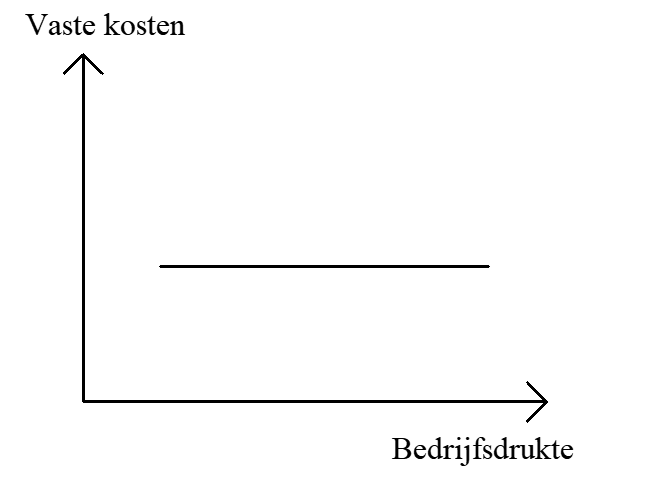
\includegraphics[width=0.35\textwidth]{assets/vastekosten.png}
    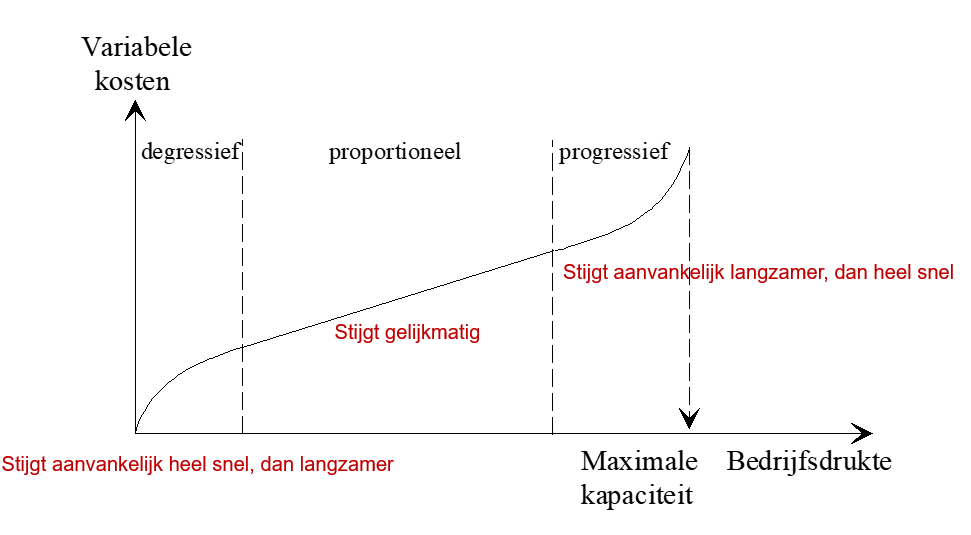
\includegraphics[width=0.55\textwidth]{assets/image3.png}
    \caption{Vaste en variabele kosten}
    \label{fig:vastevariablekosten}
\end{figure}
\FloatBarrier

\begin{itemize}
    \item \textbf{Degressief:} In het begin gaan de totale kosten snel omhoog,
          omdat sommige zaken (de oven aanzetten) al veel kosten voor de eerste stuks.
          Per eenheid dalen de kosten dus naarmate je meer produceert.
    \item \textbf{Proportioneel:} De kosten stijgen recht evenredig met de productie.

    \item \textbf{Progressief:}
          Vanaf een punt ga je teveel produceren.
          Je oven en kok moeten bijvoorbeeld overuren draaien
          waardoor je meer moet betalen of je meer
          onderhoud moet doen.
          Je gaat dus meer betalen per extra eenheid.

\end{itemize}

$\Rightarrow$ Er is dus een optimaal punt waar je kostprijs per eenheid het laagst is.

\begin{examenbox}
    Deze grafieken moet je kunnen tekenen en uitleggen wat ze betekenen.
\end{examenbox}


\subsubsection{Fifo en Lifo}

\begin{conceptbox}


    Hoe kun je nu de waarde van je voorraad bepalen?
    Er zijn twee methodes: FIFO en LIFO:

    \textbf{FIFO} is First In First Out.
    \textbf{LIFO} is Last In First Out.
\end{conceptbox}


Stel je koopt 100 eenheden voor 10 euro per stuk en daarna 50 eenheden voor 12 euro per stuk.
Dan heb je $100 \times 10 + 50 \times 12 = 1.600$ euro uitgegeven.
Je verkoopt er 60.
\newline

\textbf{FIFO:}
Je verkoopt de eerste 60 eenheden die je gekocht hebt.
Dus $60 \times 10 = 600$ euro kostprijs.
Je hebt dan nog 40 eenheden over van 10 euro per stuk en 50 van 12 euro per stuk (waarde $400 + 600 = 1.000$ euro).
\newline

\textbf{LIFO:}
Je verkoopt de laatste 60 eenheden die je gekocht hebt.
Dus $50 \times 12 = 600$ euro plus $10 \times 10 = 100$ euro, samen 700 euro kostprijs.
Je hebt dan nog 90 eenheden over van 10 euro per stuk (waarde 900 euro).


\subsubsection{Primitieve Toeslag methodes}
\textbf{Primitieve toeslagmethode:}
Je neemt je indirecte kosten en verdeelt die met één verdeelsleutel over je producten.

\textbf{Directe kosten, indirect kosten en toeslagmethode}

De ingrediënten kosten 5000 euro.
De cola's kosten 5000 euro.
De kok kost 3000 euro.
De ober kost 2000 euro.

We verkopen 1000 pizza's.
We verkopen 2000 cola's

Directe variabele kost per pizza $= 5000/1000 = 5$ euro.
Directe variabele kost per cola $= 5000/2000 = 2{,}50$ euro.

De kok is een arbeidskost. Dit is een vaste directe kost.
De kok kost 3000/1000 = 3 euro per pizza.
De ober kost 2000/2000 = 1 euro per cola.

\textbf{Tabel 1: Directe Kosten}

\begin{table}[ht]
    \centering
    \begin{tabular}{|l|r|r|}
        \hline
        \textbf{Kostentype}          & \textbf{Pizza P} & \textbf{Cola C} \\
        \hline
        Ingrediënten (per eenheid)   & €5,00            & €2,50           \\
        Arbeid (per eenheid)         & €3,00            & €1,00           \\
        \hline
        \textbf{Totale directe kost} & \textbf{€8,00}   & \textbf{€3,50}  \\
        \hline
    \end{tabular}
    \caption{Directe Kosten per Product}
\end{table}

\textbf{Indirecte kosten}
Er zijn indirect kosten van 2000 euro.
Hoe gaan we die nu toewijzen want sommige producten zijn duurder
dan andere.

Dit noemen we de \belangrijk{toeslag}.

\[ \text{Toeslag \%} = \frac{\text{indirecte kosten}}{\text{gekozen directe kosten}} \times 100 \]
\newline

\textbf{Tabel 2: Toeslag op basis van ALLE directe kosten}

Toeslag op alle directe kosten $= \dfrac{\text{€}2000}{\text{€}15000} = 13{,}33\%$
\newline

\begin{center}
    \begin{tabular}{|l|r|r|}
        \hline
        \textbf{Kostentype}         & \textbf{Pizza P} & \textbf{Cola C} \\
        \hline
        Directe kosten ingrediënten & €5,00            & €2,50           \\
        Direct kosten arbeid        & €3,00            & €1,00           \\
        Toeslag (13,33\%)           & €1,07            & €0,47           \\
        \hline
        \textbf{Totale kostprijs}   & \textbf{€9,07}   & \textbf{€3,97}  \\
        \hline
    \end{tabular}
\end{center}
\phantomsection\label{tab:toeslag_alle_directe_kosten}
\begin{center}\small\emph{Tabel: Kostprijs met Toeslag op Alle Directe Kosten}\end{center}

\textbf{Tabel 3: Toeslag op basis van INGREDIËNTEN}

Toeslag op ingrediënten $= \dfrac{\text{€}2000}{\text{€}10000} = 20\%$
\newline

\begin{table}[ht]
    \centering
    \begin{tabular}{|l|r|r|}
        \hline
        \textbf{Kostentype}       & \textbf{Pizza P} & \textbf{Cola C} \\
        \hline
        Ingrediënten              & €5,00            & €2,50           \\
        Toeslag ingrediënten      & €1,00            & €0,50           \\
        Arbeid                    & €3,00            & €1,00           \\
        \hline
        \textbf{Totale kostprijs} & \textbf{€9,00}   & \textbf{€4,00}  \\
        \hline
    \end{tabular}
    \caption{Kostprijs met Toeslag op Ingrediënten}
\end{table}

\textbf{Tabel 4: Toeslag op basis van ARBEID}

Toeslag op arbeid $= \dfrac{\text{€}2000}{\text{€}5000} = 40\%$

\begin{table}[ht]
    \centering
    \begin{tabular}{|l|r|r|}
        \hline
        \textbf{Kostentype}       & \textbf{Pizza P} & \textbf{Cola C} \\
        \hline
        Ingrediënten              & €5,00            & €2,50           \\
        Arbeid                    & €3,00            & €1,00           \\
        Toeslag arbeid            & €1,20            & €0,40           \\
        \hline
        \textbf{Totale kostprijs} & \textbf{€9,20}   & \textbf{€3,90}  \\
        \hline
    \end{tabular}
    \caption{Kostprijs met Toeslag op Arbeid}
\end{table}

\subsubsection{Verfijnde toeslagmethode}
Hierbij verfijn je de verdeelsleutels: je splitst je indirecte kosten op in
aparte potjes (indirecte materiaalkosten, indirecte arbeid, indirect machinegebruik\dots)
en gebruikt voor elk potje een eigen toeslag met een eigen basis.
Zo krijgt een machine-intensief product ook echt meer machinekosten toegewezen.
\newline

Zie het boek of de slides voor een voorbeeld.


\subsubsection{Kostenplaatsmethode}
Hier ga je de indirecte kosten toewijzen aan verschillende kostenplaatsen.
De huur van de pizzeria is 500 euro.
Je deelt dan die 500 euro op in verschillende kostenplaatsen.
De pizza keuken, de bar, de administratie etc.
Je gaat dan per kostenplaats de indirecte kosten toewijzen.

Pizzakeuken is 60\% van de oppervlakte.
Bar is 30\% van de oppervlakte.
Administratie is 10\% van de oppervlakte.
\newline
Dus de huur van de pizzakeuken is $500 \times 0{,}6 = 300$ euro.
De huur van de bar is $500 \times 0{,}3 = 150$ euro.
De huur van de administratie is $500 \times 0{,}1 = 50$ euro.
\newline

Je kunt nog meer verdelen zoals verzekering van de machines met de waarde
van de machines.
Of elektriciteit met het verbruik van de machines.
\newline


\subsection{Kostprijsberekening methodes}
We hebben nu gezien hoe je kosten over producten kunt verdelen.
Maar hoe geraken we nu tot een kostprijsberekening?
Er zijn verschillende methodes om dit te doen.
\newline

\textit{Let op: in de cursus krijgen dezelfde methodes verderop soms een andere naam.
    Hier staan ze op een rij:}
\begin{description}
    \item \concept{Klassieke kostprijsberekening}: Je kijkt naar
          alle kosten die gemaakt zijn en deelt die door de geproduceerde eenheden.
          De winst die je dan maakt is de \belangrijk{handelswinst}
    \item \concept{Industriële kostprijsberekening}
          Alle kosten door de grondstoffen, arbeid, en productie.
          De winst die je dan maakt is de \belangrijk{exploitatiewinst}

          \textit{Exploitatiewinst omdat je puur kijkt naar de productie maar je hebt nog geen verkoopkosten en
              algemene kosten meegerekend.}
    \item \concept{Evenredige kostprijsberekening}:
          Je kijkt enkel naar de kosten die evenredig meelopen met de productie
          (gebruikte grondstoffen en lonen); productie- en verkoopkosten die vast zijn, laat je eruit.
          Wat je dan overhoudt is de \belangrijk{marge} (dekkingsbijdrage).
          \textit{Dat is dus nog geen winst, maar wat er per stuk overblijft om de vaste kosten te dekken.}

\end{description}

\begin{figure}[ht]
    \centering
    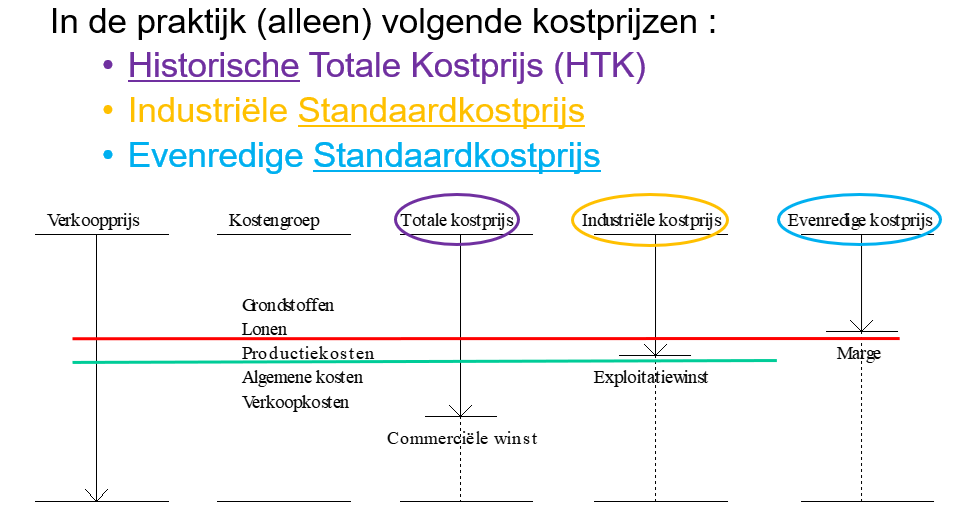
\includegraphics[width=0.8\textwidth]{assets/VerschillendeMethodes.png}
    \caption{}
    \label{fig:VerschillendeMethodes.png}
\end{figure}
\FloatBarrier


Elk van deze kostprijzen hangen af van wat er in het verleden
gebeurd is \belangrijk{(historische kostprijsberekening)}.
Wanneer je in plaats daarvan met standaardprijzen werkt
voor de grondstoffen die je gebruikt (wat kost 1 kg staal volgens de norm?),
dan spreken we van \belangrijk{standaard kostprijsberekening}.


\begin{description}
    \item\concept{Historische kostprijsberekening:} Hierbij bereken je de kostprijs op basis van de
          werkelijke kosten die gemaakt zijn in het verleden.
          Deze kunnen verschillen van de geplande kosten.
          \newline

          Deze kostprijsberekening hangt af van het verleden
          en is dus niet altijd representatief voor de toekomst:
          lonen en grondstofprijzen kunnen veranderen.
          Efficiëntie kun je hier ook niet mee meten want als je in het verleden
          inefficiënt was, dan is dat gewoon in de kostprijs verwerkt.
          \newline
          Historische kostprijzen tellen gewoon alle gemaakte kosten op.
          Je krijgt dus geen zicht op de opsplitsing in vaste en variabele kosten.

          \begin{oefenblok}[Oefening: Wijnhandelaar - Toeslagen en Productmix]
              \textbf{Situatie:}

              Een wijnhandelaar verkoopt twee soorten wijn in flessen van 1 liter:

              \textbf{Gegeven:}
              \begin{itemize}
                  \item \textbf{Wijn A:} 50 liter à €80/liter = €4.000 inkoop
                  \item \textbf{Wijn B:} 50 liter à €120/liter = €6.000 inkoop
                  \item \textbf{Directe kosten} (flessen + arbeid): €10 per fles
                  \item \textbf{Vaste kosten} (huur): €4.000
                  \item \textbf{Verkoopprijs A:} €135 per fles
                  \item \textbf{Verkoopprijs B:} €175 per fles
              \end{itemize}

              \textbf{Gevraagd:} Bereken de kostprijs met verschillende toeslagmethoden en analyseer de productmix.

              \textbf{Oplossing - Stap 1: Basisberekeningen}

              \begin{tabular}{lcc}
                  \hline
                                                     & \textbf{Wijn A} & \textbf{Wijn B} \\
                  \hline
                  Aantal flessen                     & 50              & 50              \\
                  Inkoop per fles                    & €80             & €120            \\
                  Directe kosten per fles            & €10             & €10             \\
                  \textbf{Variabele kosten per fles} & \textbf{€90}    & \textbf{€130}   \\
                  \hline
              \end{tabular}

              Totale vaste kosten (huur): €4.000 moeten worden toegerekend.

              \textbf{Stap 2: Methode 1 - Gelijkmatige verdeling}

              Vaste kosten per fles: €4.000 ÷ 100 flessen = €40/fles

              \begin{tabular}{lcc}
                  \hline
                                              & \textbf{Wijn A} & \textbf{Wijn B} \\
                  \hline
                  Variabele kosten            & €90             & €130            \\
                  Vaste kosten (toeslag)      & €40             & €40             \\
                  \textbf{Kostprijs per fles} & \textbf{€130}   & \textbf{€170}   \\
                  Verkoopprijs                & €135            & €175            \\
                  \textbf{Winst per fles}     & \textbf{€5}     & \textbf{€5}     \\
                  \hline
              \end{tabular}

              \textbf{Stap 3: Methode 2 - Toeslag op variabele kosten}

              Totale variabele kosten: (50 × €90) + (50 × €130) = €11.000

              Toeslagpercentage: €4.000 ÷ €11.000 = 36,36\%

              \begin{tabular}{lcc}
                  \hline
                                              & \textbf{Wijn A}  & \textbf{Wijn B}  \\
                  \hline
                  Variabele kosten            & €90              & €130             \\
                  Vaste kosten (36,36\%)      & €32,73           & €47,27           \\
                  \textbf{Kostprijs per fles} & \textbf{€122,73} & \textbf{€177,27} \\
                  Verkoopprijs                & €135             & €175             \\
                  \textbf{Winst per fles}     & \textbf{€12,27}  & \textbf{-€2,27}  \\
                  \hline
              \end{tabular}

              \textbf{Analyse:} Bij deze methode lijkt Wijn B verlieslatend!

              \textbf{Stap 4: Wat als we Wijn B schrappen?}

              Als we Wijn B schrappen en alleen Wijn A verkopen:

              \begin{tabular}{lc}
                  \hline
                                              & \textbf{Alleen Wijn A} \\
                  \hline
                  Omzet (50 × €135)           & €6.750                 \\
                  Variabele kosten (50 × €90) & €4.500                 \\
                  \textbf{Dekkingsbijdrage}   & \textbf{€2.250}        \\
                  Vaste kosten                & €4.000                 \\
                  \textbf{Resultaat}          & \textbf{-€1.750}       \\
                  \hline
              \end{tabular}

              \textbf{Met beide producten:}

              \begin{tabular}{lc}
                  \hline
                                                   & \textbf{Beide wijnen} \\
                  \hline
                  Omzet A (50 × €135)              & €6.750                \\
                  Omzet B (50 × €175)              & €8.750                \\
                  \textbf{Totale omzet}            & \textbf{€15.500}      \\
                  Variabele kosten A               & €4.500                \\
                  Variabele kosten B               & €6.500                \\
                  \textbf{Totale variabele kosten} & \textbf{€11.000}      \\
                  \textbf{Dekkingsbijdrage}        & \textbf{€4.500}       \\
                  Vaste kosten                     & €4.000                \\
                  \textbf{Resultaat}               & \textbf{+€500}        \\
                  \hline
              \end{tabular}

              \textbf{Conclusie:}
              \begin{itemize}
                  \item Wijn B draagt €45 per fles bij aan de vaste kosten (€175 - €130)
                  \item Zonder Wijn B maak je €1.750 verlies in plaats van €500 winst
                  \item Het schrappen van een "verlieslatend" product is gevaarlijk als het nog een positieve dekkingsbijdrage heeft
                  \item De toeslagmethode beïnvloedt sterk welk product "winstgevend" lijkt
              \end{itemize}
          \end{oefenblok}


          Door al deze problemen wordt gekeken naar een andere methode:
    \item\concept{(Industriële)Standaard kostprijsberekening:} Je kijkt naar
          alle elementen die in de kostprijs zitten
          en bekijken wat de standaard kosten zijn.
          Je gaat dus kijken naar de standaard prijzen van grondstoffen,
          standaard lonen, standaard machine gebruik etc.
          \newline

          \begin{oefenblok}[Oefening: Industriële Standaard Kostprijsberekening]
              \textbf{Voorbeeld: De Smederij - Industriële Standaardkostprijs}

              Bij de industriële standaardkostprijs wordt de kostprijs vooraf berekend op basis van technische standaarden,
              in plaats van achteraf op basis van werkelijke uitgaven. De kostprijs werkt met kostenplaatsen en standaarden,
              en blijft geldig zolang de standaarden niet wijzigen.

              \textbf{Gegeven:}

              Een smederij produceert een metalen component met de volgende technische gegevens:
              \begin{itemize}
                  \item Aantal uren smeden: 3,5 uur
                  \item Gewicht voor thermische behandeling: 12 kg
                  \item Standaardprijs smeden: €45 per uur
                  \item Standaardprijs thermische behandeling: €8 per kg
              \end{itemize}

              \textbf{Gevraagd:} Bereken de industriële standaardkostprijs voor dit product.

              \textbf{Oplossing:}

              De industriële standaardkostprijs wordt berekend als:
              \begin{align*}
                  \text{Standaardkostprijs} & = (\text{Uren smeden} \times \text{Std. prijs/uur})         \\
                                            & \quad + (\text{Kg behandeling} \times \text{Std. prijs/kg})
              \end{align*}

              Invullen van de gegevens:
              \begin{align*}
                  \text{Standaardkostprijs} & = (3,5 \text{ uur} \times €45/\text{uur}) + (12 \text{ kg} \times €8/\text{kg}) \\
                                            & = €157,50 + €96,00                                                              \\
                                            & = \mathbf{€253,50}
              \end{align*}

              \textbf{Interpretatie:}

              De vooraf bepaalde kostprijs voor dit product is €253,50. Deze standaardkostprijs geldt als norm.
              Achteraf worden de werkelijke kosten vergeleken met deze standaard. Als de werkelijke kosten:
              \begin{itemize}
                  \item \textbf{Lager} zijn dan €253,50: positieve afwijking (efficiëntie)
                  \item \textbf{Hoger} zijn dan €253,50: negatieve afwijking (inefficiëntie)
              \end{itemize}

              \textbf{Voorbeeld afwijkingsanalyse:}

              Stel dat de werkelijke kosten achteraf:
              \begin{itemize}
                  \item Werkelijke uren smeden: 4 uur à €45/uur = €180
                  \item Werkelijke kg behandeling: 12 kg à €9/kg = €108
                  \item Totale werkelijke kosten: €288
              \end{itemize}

              Afwijking: €288 - €253,50 = \textbf{€34,50 negatieve afwijking}

              Deze afwijking kan worden opgesplitst:
              \begin{itemize}
                  \item Tijdsafwijking smeden: (4 - 3,5) × €45 = €22,50 (inefficiënt)
                  \item Prijsafwijking behandeling: 12 × (€9 - €8) = €12,00 (hogere prijs)
              \end{itemize}
          \end{oefenblok}


    \item\concept{Evenredige kostprijsberekening:}
          De industriële kostprijsberekening is ook niet perfect.
          Je hebt bijvoorbeeld geen idee van hoeveel producten
          je moet verkopen om winst te maken.
          De evenredige kosten biedt antwoord op de vragen:
          Hoeveel kan ik afzetten (verkopen) voordat ik winst maak?
          Hoe rendabel is mijn product?
          \newline
          Je kijkt dus naar de vaste en variabele kosten
          en doet een \belangrijk{break-evenanalyse}.



          \textbf{Break-Even Analyse}
          \newline
          De break-even analyse bepaalt het punt waarop een bedrijf geen winst of verlies maakt. Dit is het moment waarop de \textbf{Totale Opbrengst (TO)} gelijk is aan de \textbf{Totale Kosten (TK)}.

          \begin{figure}[ht]
              \centering
              \begin{minipage}{0.45\textwidth}
                  \textbf{Kernbegrippen:}
                  \begin{description}
                      \item[\concept{Dekkingsbijdrage}] Dit is het verschil tussen de verkoopprijs en de variabele kosten ($P - VCK$). Dit bedrag per verkocht stuk draagt bij aan het dekken van de vaste kosten.
                      \item[\concept{Break-Even Afzet ($Q_{BE}$)}] Het aantal stuks dat verkocht moet worden:
                            \[ Q_{BE} = \frac{TCK}{P - VCK} \]
                      \item[\concept{Break-Even Omzet ($TO_{BE}$)}] De omzet in euro's waarbij winst nul is:
                            \[ TO_{BE} = P \times Q_{BE} \]
                      \item[\concept{Veiligheidsmarge}] Hoeveel de afzet mag dalen voordat er verlies wordt gemaakt (vaak uitgedrukt in \% van de huidige afzet).
                  \end{description}
              \end{minipage}%
              \hfill
              \begin{minipage}{0.5\textwidth}
                  \centering
                  \begin{tikzpicture}[scale=0.8, >=stealth]
                      % Axes
                      \draw[->, thick] (0,0) -- (6,0) node[right] {Q (Aantal)};
                      \draw[->, thick] (0,0) -- (0,5) node[above] {€};

                      % TCK (Fixed Costs)
                      \draw[thick, schoolBlue] (0,1.5) -- (5.5,1.5) node[right, font=\tiny] {TCK};

                      % TK (Total Costs)
                      \draw[thick, schoolOrange] (0,1.5) -- (5.5,4.25) node[right, font=\tiny] {TK};

                      % TO (Revenue)
                      \draw[thick, teal!80!black] (0,0) -- (5,5) node[right, font=\tiny] {TO};

                      % BEP
                      \fill[black] (3,3) circle (2pt);
                      \node[above left, font=\bfseries\scriptsize] at (3,3) {BEP};

                      \fill[schoolRed, opacity=0.15] (0,0) -- (3,3) -- (0,1.5) -- cycle;
                      \node[schoolRed, font=\tiny] at (1, 1.8) {Verlies};

                      \fill[teal, opacity=0.15] (3,3) -- (5,5) -- (5,4) -- cycle;
                      \node[teal!80!black, font=\tiny] at (4.5, 3.8) {Winst};

                      \draw[dashed] (3,3) -- (3,0) node[below, font=\scriptsize] {$Q_{BE}$};
                  \end{tikzpicture}
                  \caption{Visualisatie van de Break-Even Analyse}
                  \label{fig:breakeven-realistic}
              \end{minipage}
          \end{figure}
          \FloatBarrier

          In de realiteit zijn deze grafieken niet lineair, omdat de variabele kosten mee veranderen met de
          productie (zie figuur~\ref{fig:vastevariablekosten}).
          Je wilt rond $q_2$ zitten: daar is het verschil tussen opbrengst en kosten het grootst.

          \begin{figure}[htbp]
              \centering
              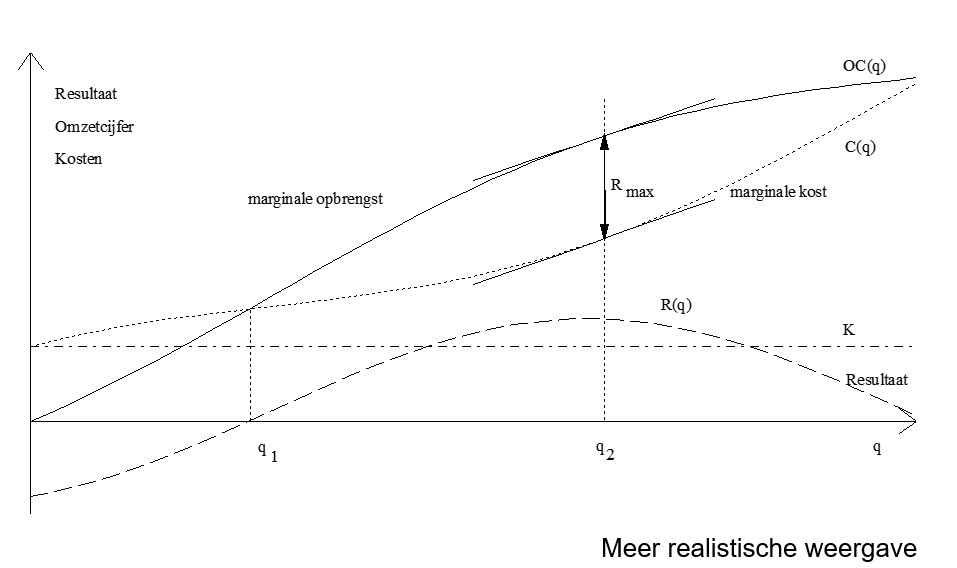
\includegraphics[width=0.7\textwidth]{assets/breakevenrealistisch.png}
              \caption{Realistische Break-Even Analyse}
              \label{fig:breakevenrealistisch.png}
          \end{figure}
          \FloatBarrier

          Je gaat dan het verschil met de marginale kost en de marginale opbrengst bekijken en dan de winst maximaliseren.
\end{description}

\begin{examenbox}
    Zorg dat je alle methodes kent en wat ze inhouden.
    Ken ook de voordelen en nadelen, en hoe de winst bij elke methode heet.
    Kijk naar figuur~\ref{fig:VerschillendeMethodes.png}:
    \begin{itemize}
        \item Exploitatiewinst (industriële kostprijsberekening)
        \item Commerciële winst / handelswinst (klassieke kostprijsberekening)
        \item Marge (evenredige kostprijsberekening)
    \end{itemize}
\end{examenbox}

\begin{examenbox}
    Zorg dat je deze grafieken goed kunt uitleggen
\end{examenbox}

\subsection{Afwijkingsanalyse}
Je wilt weten of je vooraf gemaakte berekening wel klopt met de werkelijke kostprijs.
Na afloop van de periode maak je die vergelijking.

\frm{Afwijkingsanalyse}{
    W = K' - K = (p' - p)\,q' + (q' - q)\,p
}
{met $W$ de totale afwijking in euro's, $K' = p'q'$ de werkelijke kosten, $K = pq$ de geraamde kosten,
    $p'$ de werkelijke prijs, $p$ de standaardprijs, $q'$ de werkelijke hoeveelheid en $q$ de standaardhoeveelheid.
    De eerste term $(p'-p)\,q'$ is de \emph{prijsafwijking}, de tweede term $(q'-q)\,p$ de
    \emph{efficiëntieafwijking}. Let op: de prijsafwijking rekent met de werkelijke hoeveelheid $q'$,
    de efficiëntieafwijking met de standaardprijs $p$. Anders tel je hetzelfde stuk twee keer.}


\begin{oefenblok}[Afwijkingsanalyse - Begroting vs Realisatie]
    \textbf{Situatie:}

    Een productiebedrijf wil de verschillen tussen begroting en werkelijkheid analyseren.

    \textbf{1. Standaarden (Begroting):} Productie van 140.000 stuks

    \begin{tabular}{lcc}
        \hline
        \textbf{Element} & \textbf{Standaard per stuk} & \textbf{Standaardprijs} \\
        \hline
        Grondstof        & 0,3 kg                      & €50/kg                  \\
        Arbeid           & 0,1 uur                     & €200/uur                \\
        Vaste kosten     & €5/stuk                     & €700.000 totaal         \\
        \hline
    \end{tabular}

    \textbf{2. Werkelijkheid (Realisatie):} Productie van 150.000 stuks

    \begin{tabular}{lcc}
        \hline
        \textbf{Element} & \textbf{Werkelijk verbruik} & \textbf{Werkelijke kosten} \\
        \hline
        Grondstof        & 43.000 kg                   & €2.080.000                 \\
        Arbeid           & 16.000 uur                  & €3.360.000                 \\
        Vaste kosten     & -                           & €700.000                   \\
        \hline
    \end{tabular}

    \textbf{3. Afwijkingsanalyse:}

    \textbf{A. Grondstoffen}

    Werkelijke prijs: $P' = \frac{€2.080.000}{43.000\text{ kg}} = €48,37/\text{kg}$

    Standaard hoeveelheid voor 150.000 stuks: $Q = 150.000 \times 0,3 = 45.000$ kg

    \begin{align*}
        \text{Prijsafwijking} & = (P' - P) \times Q'                                                     \\
                              & = (€48,37 - €50) \times 43.000                                           \\
                              & = \mathbf{-€70.000} \quad \text{\textcolor{green!70!black}{(Voordelig)}}
    \end{align*}

    \textit{Interpretatie:} Grondstoffen goedkoper ingekocht dan gepland.

    \begin{align*}
        \text{Efficiëntieafwijking} & = (Q' - Q) \times P                                                       \\
                                    & = (43.000 - 45.000) \times €50                                            \\
                                    & = \mathbf{-€100.000} \quad \text{\textcolor{green!70!black}{(Voordelig)}}
    \end{align*}

    \textit{Interpretatie:} Minder materiaal verbruikt (43.000 kg) dan de standaard (45.000 kg).

    \textbf{Totale afwijking grondstoffen:} -€70.000 + (-€100.000) = \textbf{-€170.000 (Voordelig)}

    \textbf{B. Arbeid}

    Werkelijk uurloon: $P' = \frac{€3.360.000}{16.000\text{ uur}} = €210/\text{uur}$

    Standaard uren voor 150.000 stuks: $Q = 150.000 \times 0,1 = 15.000$ uur

    \begin{align*}
        \text{Prijsafwijking} & = (P' - P) \times Q'                                         \\
                              & = (€210 - €200) \times 16.000                                \\
                              & = \mathbf{+€160.000} \quad \text{\textcolor{red}{(Nadelig)}}
    \end{align*}

    \textit{Interpretatie:} Personeel was duurder per uur dan begroot.

    \begin{align*}
        \text{Efficiëntieafwijking} & = (Q' - Q) \times P                                          \\
                                    & = (16.000 - 15.000) \times €200                              \\
                                    & = \mathbf{+€200.000} \quad \text{\textcolor{red}{(Nadelig)}}
    \end{align*}

    \textit{Interpretatie:} Personeel werkte trager dan standaard (16.000 uur i.p.v. 15.000 uur).

    \textbf{Totale afwijking arbeid:} +€160.000 + €200.000 = \textbf{+€360.000 (Nadelig)}

    \textbf{C. Vaste Kosten (Capaciteit)}

    Standaard vaste kosten per stuk: $\frac{€700.000}{140.000} = €5/\text{stuk}$

    \begin{align*}
        \text{Bezettingsafwijking} & = (\text{Geplande productie} - \text{Werkelijke productie}) \times \text{Std. tarief} \\
                                   & = (140.000 - 150.000) \times €5                                                       \\
                                   & = \mathbf{-€50.000} \quad \text{\textcolor{green!70!black}{(Voordelig)}}
    \end{align*}

    \textit{Interpretatie:} Meer geproduceerd (150k vs 140k), dus vaste kosten gespreid over meer eenheden.

    \textbf{Totaaloverzicht:}

    \begin{tabular}{lrr}
        \hline
        \textbf{Kostensoort}       & \textbf{Afwijking} & \textbf{Effect}  \\
        \hline
        Grondstoffen - Prijs       & -€70.000           & Voordelig        \\
        Grondstoffen - Efficiëntie & -€100.000          & Voordelig        \\
        Arbeid - Prijs             & +€160.000          & Nadelig          \\
        Arbeid - Efficiëntie       & +€200.000          & Nadelig          \\
        Vaste kosten - Bezetting   & -€50.000           & Voordelig        \\
        \hline
        \textbf{Totale afwijking}  & \textbf{+€140.000} & \textbf{Nadelig} \\
        \hline
    \end{tabular}

    \textbf{Conclusie:}
    \begin{itemize}
        \item De arbeidskosten vielen veel hoger uit (+€360.000) door hogere lonen én inefficiënt werken
        \item Dit werd deels gecompenseerd door:
              \begin{itemize}
                  \item Goedkopere inkoop grondstoffen (-€70.000)
                  \item Zuiniger materiaalgebruik (-€100.000)
                  \item Hogere productievolume (-€50.000)
              \end{itemize}
        \item Netto resultaat: €140.000 meer kosten dan begroot
        \item Actie nodig: Arbeidsefficiëntie verbeteren en loonkosten onderzoeken
    \end{itemize}
\end{oefenblok}



\subsection{Activity Based Costing (ABC)}
Al deze kostprijsberekeningen geven weinig inzicht in wat één specifiek product echt kost.
Stel dat je twee producten hebt die heel andere processen doorlopen: met de vorige methodes
verdeel je de indirecte kosten met één grove sleutel, zonder te kijken wat die kosten
werkelijk veroorzaakt.
Bij \belangrijk{ABC} wijs je de kosten toe per \textbf{activiteit} (de cost driver),
en pas daarna per product op basis van hoeveel het van die activiteit verbruikt.
Dat is veel realistischer, maar ook een pak moeilijker te implementeren: je moet
per activiteit meten.
\newline


\begin{oefenblok}[Oefening uit examen: Activity Based Costing (ABC)]
    \textbf{Situatie:}

    Het maken van product A en B kost 3.500 euro aan indirecte kosten in totaal.

    Deze kosten zijn onderverdeeld in drie activiteiten:
    \begin{itemize}
        \item Machine-uren: €2.000
        \item Inspecties: €1.000
        \item Verpakkingen: €500
    \end{itemize}

    De producten verbruiken de activiteiten als volgt:

    \begin{tabular}{lcc}
        \hline
        \textbf{Activiteit} & \textbf{Product A} & \textbf{Product B} \\
        \hline
        Machine-uren        & 100 uur            & 50 uur             \\
        Inspecties          & 10 keer            & 30 keer            \\
        Verpakkingen        & 200 stuks          & 100 stuks          \\
        \hline
    \end{tabular}

    \vspace{4mm}
    \textbf{Oplossing:}

    Stap 1: Bepaal de cost-driver tarieven
    \begin{itemize}
        \item Machine-uren: totaal = $100 + 50 = 150$ uur. Tarief = $\frac{2000}{150} = €13{,}333\ldots$ (afronden op twee decimalen: €13,33/uur).
        \item Inspecties: totaal = $10 + 30 = 40$ keer. Tarief = $\frac{1000}{40} = \mathbf{€25{,}00}$ per inspectie.
        \item Verpakkingen: totaal = $200 + 100 = 300$ stuks. Tarief = $\frac{500}{300} = €1{,}666\ldots$ (afronden: €1,67/stuk).
    \end{itemize}

    Stap 2: Toewijzen van kosten per product (afrondingen zo dat totalen optellen)

    \begin{tabular}{llr}
        \hline
        \textbf{Activiteit}                           & \textbf{Berekening}         & \textbf{Toegewezen}  \\
        \hline
        \multicolumn{3}{l}{\textbf{Product A}}                                                              \\
        Machine-uren (tarief €13,333\dots)            & $100 \times €13{,}333$      & €1.333,33            \\
        Inspecties (tarief €25,00)                    & $10 \times €25{,}00$        & €250,00              \\
        Verpakkingen (tarief €1,666\dots)             & $200 \times €1{,}667$       & €333,33              \\
        \hline
        \textbf{Totaal Product A}                     &                             & \textbf{€1.916,66}   \\
        \hline
        \multicolumn{3}{l}{\textbf{Product B}}                                                              \\
        Machine-uren (tarief €13,333\dots)            & $50 \times €13{,}333$       & €666,67              \\
        Inspecties (tarief €25,00)                    & $30 \times €25{,}00$        & €750,00              \\
        Verpakkingen (tarief €1,666\dots)             & $100 \times €1{,}667$       & €166,67              \\
        \hline
        \textbf{Totaal Product B}                     &                             & \textbf{€1.583,34}   \\
        \hline
        \textbf{Controle (som)}                       &                             & \textbf{€3.500,00}   \\
        \hline
    \end{tabular}

    \vspace{2mm}
    \textbf{Conclusie:} Via ABC krijgen we de volgende toewijzing van de €3.500 aan indirecte kosten:
    \begin{itemize}
        \item Product A: €1.916,66
        \item Product B: €1.583,34
    \end{itemize}

\end{oefenblok}

Bekijk de slides of het boek voor extra voorbeelden van ABC.

\begin{examenbox}
    Op het examen moet je sowieso een traditionele kostprijsberekening
    en/of een ABC-kostprijsberekening kunnen maken.
\end{examenbox}
\subsection{Target based costing}

Bij traditionele kostprijsberekening maak je je product en kijk je daarna wat de kost is.
Bij target based costing ga je eerst kijken wat de marktprijs is.
Je kijkt dus wat de klant wil betalen voor een product.
Daarna ga je je product maken binnen die kostprijs.
Dit is dus een omgekeerde manier van denken.

\begin{figure}[ht]
    \centering
    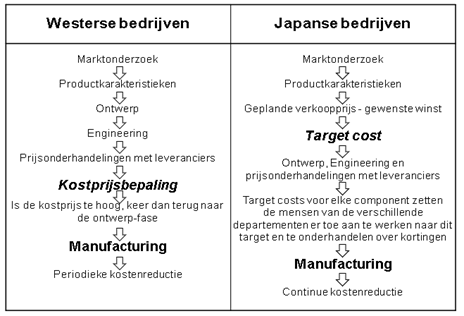
\includegraphics[width=0.6\textwidth]{assets/image6.png}
    \caption{}
    \label{fig:image6.png}
\end{figure}
\FloatBarrier



\section{Module 5: Analyse van een jaarrekening}

Een paar belangrijke termen om te kennen:
\begin{itemize}
    \item Balans: Een momentopname van de financiële
          situatie van een bedrijf op een bepaald tijdstip.
          Dit is een foto van de activa en passiva.
    \item Resultatenrekening: Een overzicht van de inkomsten en uitgaven over een bepaalde periode.
          Dit is een video van de winst en verlies.
    \item Toelichting: Uitleg en details bij de balans en resultatenrekening.
    \item Sociale balans: Een overzicht van de sociale aspecten van een bedrijf,
          zoals arbeidsomstandigheden en personeelsbeleid.
    \item Niet-financiële informatie: Informatie die niet direct in geld kan worden uitgedrukt,
          zoals milieubeleid en maatschappelijke verantwoordelijkheid.
\end{itemize}


De boekhouding volgt vaste principes: je moet dezelfde kosten elk jaar op dezelfde manier boeken
(het bestendigheidsbeginsel). Alleen zo kun je ratio's tussen jaren zinvol vergelijken.

\begin{examenbox}
    Een vraag uit een examen kan zijn: \textit{``Waarom worden ratio-analyses gebruikt binnen het financieel
        management? Wat zijn de beperkingen? Leg uit.''}
\end{examenbox}


Activa is wat een bedrijf bezit.
Passiva is hoe dat gefinancierd is.
Ezelsbruggetje: passiva zijn passief (het geld staat er alleen maar, het komt ergens vandaan),
activa zijn actief (daarmee doet het bedrijf iets).



\begin{conceptbox}
    \subsubsection{Activa (Wat bezit het bedrijf?)}
    \begin{itemize}
        \item \textbf{Vaste activa:} Lange termijn investeringen
              \begin{itemize}
                  \item Gebouwen, machines, voertuigen
                  \item Immateriële activa (patenten, licenties)
              \end{itemize}
        \item \textbf{Vlottende activa:} Korte termijn bezittingen
              \begin{itemize}
                  \item Voorraden (grondstoffen, halffabricaten, eindproducten)
                  \item Vorderingen (geld dat klanten nog schuldig zijn)
                  \item Bankrekening en contanten
              \end{itemize}
    \end{itemize}

    \subsubsection{Passiva (Waar komt het geld vandaan?)}

    \begin{itemize}
        \item \textbf{Eigen Vermogen:} Geld van eigenaren/aandeelhouders
              \begin{itemize}
                  \item Inbreng van oprichters
                  \item Gerealiseerde winsten (ingehouden winst)
              \end{itemize}
        \item \textbf{Vreemd Vermogen:} Geld van externe financiers
              \begin{itemize}
                  \item Langetermijnleningen (bank)
                  \item Korttermijnschulden (leveranciers, belastingen)
              \end{itemize}
    \end{itemize}
\end{conceptbox}

\begin{figure}[ht]
    \centering
    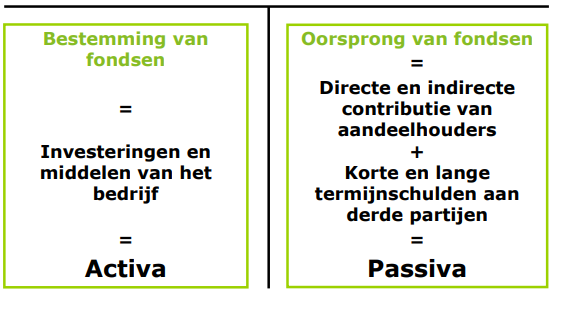
\includegraphics[width=0.8\textwidth]{assets/balans1.png}
    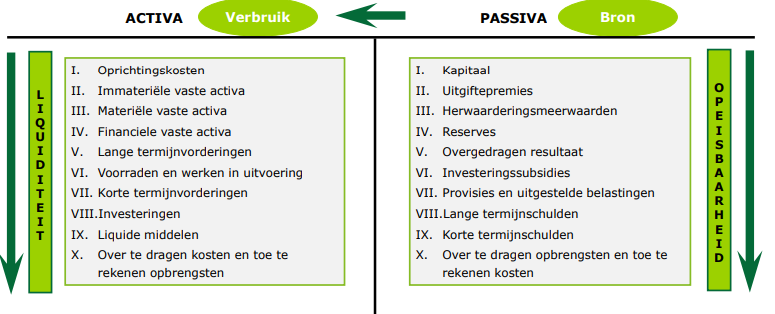
\includegraphics[width=0.8\textwidth]{assets/balans2.png}
    \caption{Voorbeeld van een Balans}
    \label{fig:balans.png}
\end{figure}
\FloatBarrier

Hoe liquider een post is, hoe sneller je er geld van kunt maken.
Vorderingen op lange termijn zijn dus moeilijker te gelde te maken
dan vorderingen op korte termijn.
\newline

De balans wordt van boven naar onder geordend volgens die liquiditeit:
bovenaan staat wat het langst vastzit, onderaan wat het snelst beschikbaar is.



\begin{figure}[ht]
    \centering
    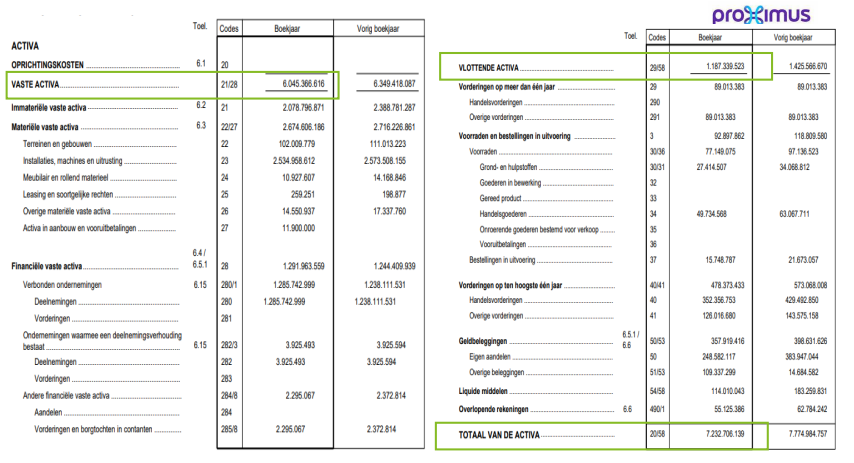
\includegraphics[width=1\textwidth]{assets/JaarrekeningPoximus.png}
    \caption{Voorbeeld van een jaarrekening van Proximus}
    \label{fig:JaarrekeningPoximus.png}
\end{figure}
\FloatBarrier

\subsection{De balans}

De balans is een \textbf{momentopname} van de financiële positie van een bedrijf op een specifiek moment (meestal aan het einde van een jaar).

\textbf{Balansformule:}
$$\textbf{Activa} = \textbf{Passiva}$$

Dit betekent: Wat een bedrijf bezit (activa) is gelijk aan waar het geld vandaan komt (passiva).


\textbf{Voorbeeld transacties:}
\begin{itemize}
    \item \textbf{Je neemt een lening van €10.000:} Bankrekening (activa) +€10.000 / Schuld (passiva) +€10.000
    \item \textbf{Je koopt een machine voor €5.000:} Machine (activa) +€5.000 / Bankrekening (activa) -€5.000 (balans blijft gelijk)
    \item \textbf{Je maakt €2.000 winst:} Bankrekening (activa) +€2.000 / Eigen vermogen (passiva) +€2.000
\end{itemize}

\subsection{Resultatenrekening}
De resultatenrekening is een film. Je neemt op tussen twee periodes. Meestal een jaar.
Je kijkt naar alle inkomsten en uitgaven tussendoor
en je bekijkt het verschil. Je \belangrijk{startkapitaal} maakt dan winst of
verlies.

De resultaat rekening wordt opgedeeld in 3 delen:
\begin{itemize}
    \item \textbf{Bedrijfsresultaat:} Dit is de winst of verlies uit de kernactiviteiten van het bedrijf.
    \item \textbf{Financieel resultaat:} Dit omvat rente-inkomsten en -kosten, evenals andere financiële opbrengsten en lasten.
    \item \textbf{Uitzonderlijk resultaat:} Dit zijn eenmalige gebeurtenissen zoals
          een ongeluk, een brand of de verkoop van een divisie: dingen die \emph{niet} elk jaar gebeuren.
\end{itemize}

Wil je weten hoe het bedrijf het echt doet, kijk dan naar het \textbf{bedrijfsresultaat}:
dat is het enige deel dat de kernactiviteit meet.

\textbf{Toelichting}
Toelichtingen zijn extra notities bij de balans en resultatenrekening.
Ze geven meer details over specifieke posten, zoals waarderingsmethoden,
risico's, en andere relevante informatie die niet direct in de cijfers zichtbaar is.
Bijvoorbeeld een grondstofcontract dat een bedrijf elke 4 jaar betaalt.
\newline

\textbf{Types jaarrekeningen:}
Jaarrekeningen zijn verplicht voor bedrijven en organisaties om
hun financiële prestaties en positie te rapporteren.
\begin{itemize}
    \item enkelvoudige jaarrekening: Dit is voor kleine bedrijven.
    \item geconsolideerde jaarrekening: Dit is voor grote bedrijven met meerdere dochterondernemingen.
\end{itemize}

Elk land heeft een eigen standaard voor jaarrekeningen. De BE GAAP is de Belgische standaard.
Internationaal is er IFRS (International Financial Reporting Standards).

\begin{figure}[ht]
    \centering
    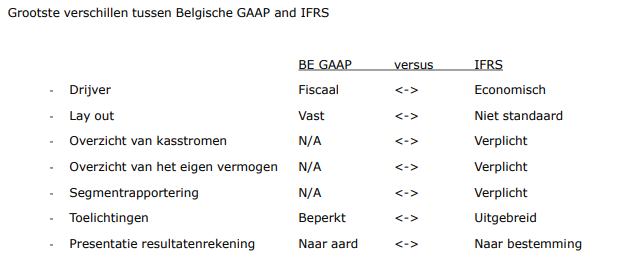
\includegraphics[width=0.8\textwidth]{assets/verschillengaap met IFRS.png}
    \caption{Structuur van een jaarrekening}
    \label{fig:jaarrekeningstructuur.png}
\end{figure}
\FloatBarrier

\textbf{Jaarverslag}:
Een verslag over de onderneming met commentaar over de jaarrekening.
Risico, continuiteit, toekomstplannen etc.
Staat een bedrijf op de beurs, dan moet het bovendien een verslag voor beursgenoteerde
ondernemingen maken. Daar staat meer in, vooral meer niet-financiële informatie.


\textbf{Commissarisverslag}:
Een auditor geeft hierin zijn opinie over de jaarrekening.
Hij controleert of de cijfers wel degelijk kloppen met de werkelijkheid van het bedrijf.
Bedrijven kunnen namelijk inkomsten opblazen of kosten verbergen.
De auditor controleert dat en maakt er een verslag over: het \belangrijk{commissarisverslag}.

\subsection{Analyse van de jaarrekening}
Jaarrekeningen worden opgesteld volgens de boekhoudkundige principes
zoals eerder vermeld.
Een bedrijf wordt bijna nooit verkocht tegen zijn boekhoudkundige waarde;
meestal ligt de verkoopprijs een stuk hoger.
\newline

Dit komt omdat bedrijven verkocht worden
op basis van hun winstgevendheid en groeipotentieel,
opinie en reputatie\dots
Een jaarrekening geeft alleen zicht op het verleden.
\newline
Om de jaarrekeningen te analyseren ga je een financiële analyse doen.

\subsection{Types van financiële analyse}
\begin{description}
    \item [Horizontale analyse:] Vergelijkt cijfers over meerdere jaren om trends te identificeren.
    \item [Verticale analyse:] Analyseert de verhouding van elk item ten opzichte van een basispost binnen hetzelfde jaar.
    \item [Ratio-analyse:] Berekenen van financiële ratio's om de prestaties en gezondheid van het bedrijf te beoordelen.
\end{description}
Er zijn er meer, maar in de cursus zien we deze drie.
\newline

Een ratio op zich zegt niets. Hij krijgt pas betekenis als je hem vergelijkt:
met vorige jaren, met de sector of met een concurrent.

\subsection{Horizontale analyse}
Je maakt een vergelijking van twee periodes.
Je kunt dit doen in percentages (groei van omzet)
of in absolute waarden (verschil in winst).

\textbf{Voorbeeld: Horizontale analyse van balansposten}

\begin{table}[ht]
    \centering
    \begin{tabular}{|l|r|r|r|r|}
        \hline
        \textbf{Balanspost}    & \textbf{Jaar 1}   & \textbf{Jaar 2}   & \textbf{Absolute Wijziging} & \textbf{Percentage \%} \\
        \hline
        Vaste activa           & €100.000          & €120.000          & +€20.000                    & +20\%                  \\
        Voorraden              & €50.000           & €55.000           & +€5.000                     & +10\%                  \\
        Vorderingen            & €30.000           & €42.000           & +€12.000                    & +40\%                  \\
        Bankrekening           & €20.000           & €18.000           & -€2.000                     & -10\%                  \\
        \hline
        \textbf{TOTAAL ACTIVA} & \textbf{€200.000} & \textbf{€235.000} & \textbf{+€35.000}           & \textbf{+17,5\%}       \\
        \hline
    \end{tabular}
    \caption{Voorbeeld Horizontale Analyse}
\end{table}

\textbf{Formules:}
\begin{itemize}
    \item \textbf{Absolute wijziging:} Jaar 2 - Jaar 1
    \item \textbf{Percentage wijziging:} $\frac{\text{Jaar 2} - \text{Jaar 1}}{\text{Jaar 1}} \times 100\%$
\end{itemize}

\textbf{Interpretatie:}
\begin{itemize}
    \item Vaste activa zijn met 20\% gestegen $\rightarrow$ bedrijf investeert in uitbreiding
    \item Vorderingen zijn met 40\% gestegen $\rightarrow$ klanten betalen trager (opletten!)
    \item Bankrekening daalt $\rightarrow$ liquide middelen nemen af (liquiditeitsrisico)
    \item Totale activa groeien met 17,5\% $\rightarrow$ het bedrijf groeit
\end{itemize}


\subsection{Verticale analyse}
Je drukt elke post uit als percentage van een totaal binnen hetzelfde jaar:
elke activapost t.o.v.\ de totale activa, elke passivapost t.o.v.\ het totale vermogen,
elke kostenpost t.o.v.\ de omzet\dots

\begin{figure}[ht]
    \centering
    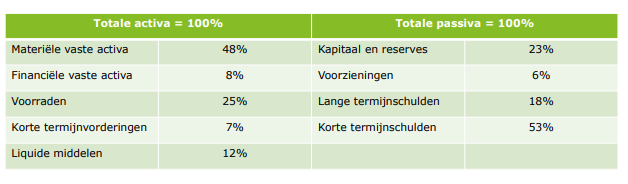
\includegraphics[width=0.45\textwidth]{assets/activapassiveanalyse.png}
    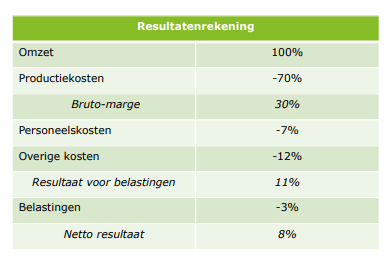
\includegraphics[width=0.45\textwidth]{assets/omzetanaluse.png}
    \caption{Voorbeeld van een verticale analyse}
    \label{fig:verticaleanalyse.png}
\end{figure}
\FloatBarrier

Je kunt dan deze analyses combineren
\begin{figure}[ht]
    \centering
    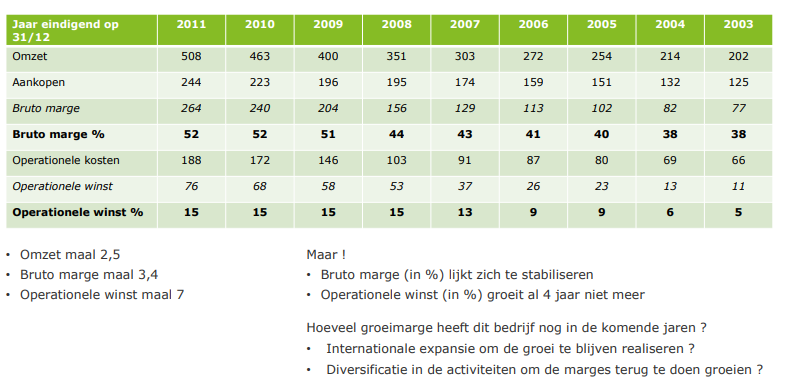
\includegraphics[width=1\textwidth]{assets/hor+vert.png}
    \caption{Combinatie van horizontale en verticale analyse}
    \label{fig:hor+vert.png}
\end{figure}
\FloatBarrier


\subsection{Ratio-analyse}
Door ratio-analyse te doen over meerdere jaarrekeningen
kun je de gezondheid van een bedrijf beoordelen.

\begin{description}

    \item[Financiele ratio's:\newline]
          \begin{itemize}
              \item \textbf{Liquiditeit:} Je kijkt naar het geld. Kan het bedrijf zijn
                    kortlopende rekeningen betalen?
              \item \textbf{Solvabiliteit:} Je gaat kijken naar de schulden. Hoeveel schulden heeft het bedrijf en de mogelijkheid
                    om die terug te betalen.
              \item \textbf{Rotatie:} De efficiëntie van de activa.
          \end{itemize}

    \item[Liquiditeitsratio's:] Deze ratio toont hoe goed het bedrijf zijn schulden op korte termijn
          kan betalen met zijn activa op korte termijn (cash, vorderingen op korte termijn en voorraden).

          \frm{Liquiditeit: current ratio}{
              \text{current ratio} = \frac{\text{vorderingen KT} + \text{cash} + \text{voorraden}}{\text{vreemd vermogen op korte termijn}}
          }
          {De teller is de volledige vlottende activa. Is de ratio groter dan 1, dan kan het bedrijf
              zijn schulden op korte termijn betalen.}

          De acid test neemt de voorraden \emph{niet} mee, want die moet je eerst nog verkopen.
          Het is dus een strengere test.
          \frm{Liquiditeit: acid test (quick ratio)}{
              \text{acid test} = \frac{\text{vorderingen KT} + \text{cash}}{\text{vreemd vermogen op korte termijn}}
          }
          {Is deze ratio groter dan 1, dan kan het bedrijf zijn schulden op korte termijn betalen
              zonder eerst zijn voorraad te moeten verkopen.}

          \textbf{Netto werkkapitaal:}
          Het netto werkkapitaal is een andere manier om te zien of een bedrijf liquide goed zit.
          \frm{Netto werkkapitaal}{
              \text{netto werkkapitaal} = \text{vlottende activa} - \text{kortlopende schulden}
          }
          {Het netto werkkapitaal geeft aan hoeveel liquide middelen een bedrijf heeft om zijn dagelijkse
              activiteiten te financieren. Een positief netto werkkapitaal betekent dat het bedrijf voldoende
              middelen heeft om aan zijn kortlopende verplichtingen te voldoen,
              terwijl een negatief netto werkkapitaal
              kan wijzen op mogelijke liquiditeitsproblemen.}

          \begin{conceptbox}
              \textbf{Vlottende activa:} Dit zijn activa die binnen een jaar in cash kunnen worden omgezet.
              Dit omvat kasgeld, voorraden, en vorderingen.
              \newline
              \textbf{Kortlopende schulden:} Dit zijn schulden die in minder dan een jaar moeten worden terugbetaald.
          \end{conceptbox}

          \begin{figure}[ht]
              \centering
              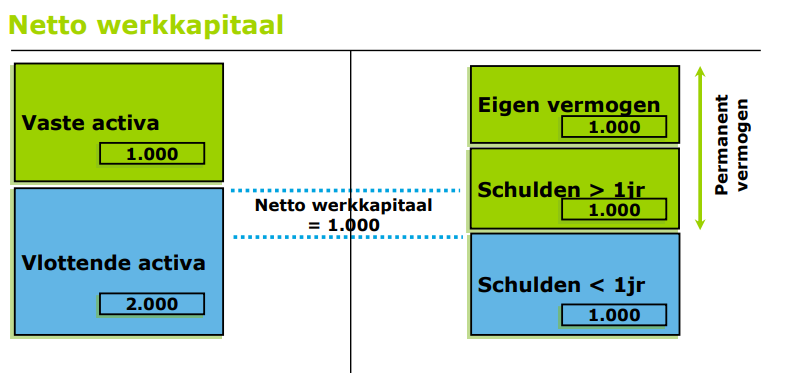
\includegraphics[width=0.8\textwidth]{assets/NettoWerkKapitaal.png}
              \caption{Netto werkkapitaal illustratie}
              \label{fig:NettoWerkKapitaal.png}
          \end{figure}

          Een positief netto werkkapitaal is het eerste teken
          van een gezond bedrijf.

          \textbf{Behoefte aan werkkapitaal}:
          \newline
          Dit is een cyclus: je koopt grondstoffen $\rightarrow$ je produceert
          $\rightarrow$ je verkoopt producten $\rightarrow$ je krijgt geld van klanten
          $\rightarrow$ je koopt weer grondstoffen.
          \newline

          Deze cyclus kan meerdere maanden duren omdat je niet direct grondstoffen
          kunt kopen, produceren en verkopen.
          Cash out is wanneer je grondstoffen koopt.
          Cash in is wanneer je geld krijgt van klanten.
          \newline
          Je moet dus genoeg Netto werkkapitaal hebben
          zodat je niet moet zitten wachten op klanten om geld te krijgen.
          \newline
          \textbf{Netto werkkapitaal $>$ behoefte aan werkkapitaal:}
          je hebt een buffer over. Daarmee kun je investeren, kaskortingen opnemen
          of vooruitbetalen aan leveranciers.
          \newline
          \textbf{Netto werkkapitaal $<$ behoefte aan werkkapitaal:}
          je moet leningen aangaan om het financiële tekort te dekken.

          \begin{figure}[ht]
              \centering
              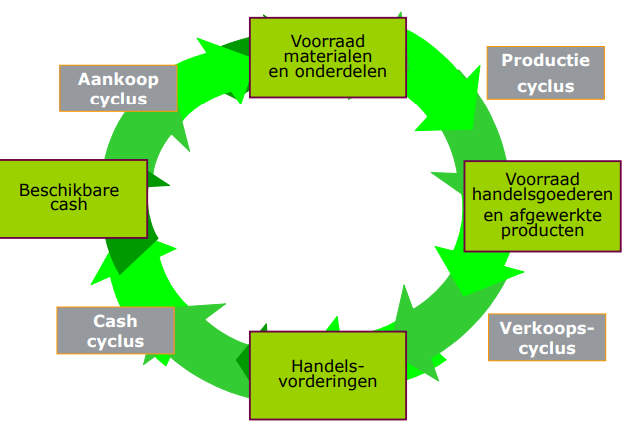
\includegraphics[width=0.6\textwidth]{assets/werkkapitaalcyclus.png}
              \caption{Werkkapitaalcyclus}
              \label{fig:werkkapitaalcyclus.png}
          \end{figure}


    \item[Efficiëntieratio's (rotatie):]
          Hoe snel roteren mijn voorraden, mijn klantenvorderingen en mijn leveranciersschulden?
          Hoe sneller het geld ronddraait, hoe meer rendement je uit dezelfde middelen haalt.

          \frm{Voorraadrotatie}{
              \text{voorraadrotatie (dagen)} = \frac{\text{gemiddelde voorraad}}{\text{kostprijs verkochte goederen}} \cdot 365
          }
          {Hoe minder dagen, hoe beter: je voorraad ligt korter stil en je hebt minder opslagkosten
              en minder vastgelegd kapitaal.}

          \frm{Klantenrotatie}{
              \text{klantenrotatie (dagen)} = \frac{\text{handelsvorderingen}}{\text{omzet}} \cdot 365
          }
          {Hoe minder dagen, hoe beter: je klanten betalen sneller, dus je krijgt je cash sneller terug
              om opnieuw te gebruiken.}

          \frm{Leveranciersrotatie}{
              \text{leveranciersrotatie (dagen)} = \frac{\text{handelsschulden}}{\text{aankopen}} \cdot 365
          }
          {Hier geldt het omgekeerde: hoe méér dagen, hoe langer je je eigen cash houdt.
              Te lang wachten schaadt wel je relatie met de leverancier.}


    \item[Solvabiliteitsratio's:]
          \belangrijk{Solvabiliteit}:

          Je hebt verschillende soorten vermogens
          \begin{itemize}
              \item \textbf{Eigen vermogen:} Geld van eigenaren/aandeelhouders
              \item \textbf{Vreemd vermogen:} Geld van externe financiers zoals banken, kan door
                    leningen of obligaties.
              \item \textbf{Totaal vermogen:} Eigen vermogen + Vreemd vermogen
          \end{itemize}

          De solvabiliteit ratio is hoeveel de onderneming zijn schuld kan
          terugbetalen met zijn eigen vermogen.


          \begin{itemize}
              \item \textbf{Dekkingsratio's}
                    \frm{Interestdekkingsratio}{
                        \text{interestdekkingsratio} = \frac{\text{operationeel resultaat (EBIT)}}{\text{interestkosten}}
                    }
                    {Het operationeel resultaat is de winst vóór interest en belastingen (EBIT).
                        Deze ratio meet hoe goed een bedrijf zijn rentelasten kan betalen met zijn operationele winst.
                        Hoe hoger, hoe beter. Een ratio lager dan 1 betekent dat je operationele winst kleiner is dan de
                        interest op je schulden; dat is niet altijd meteen dramatisch, omdat afschrijvingen en andere
                        niet-kaskosten de winst drukken zonder dat er geld wegvloeit.}

                    \frm{Operationele kasstroom versus schuld}{
                        \frac{\text{operationele kasstroom}}{\text{totale schuld}}
                    }{
                        Deze ratio meet hoe goed een bedrijf zijn totale schulden kan aflossen met de kasstroom uit
                        zijn gewone activiteiten. Hoe hoger, hoe beter. Ze is meestal kleiner dan 1, omdat de totale
                        schuld vaak groter is dan één jaar kasstroom. Een heel lage ratio wijst op problemen bij het aflossen.
                    }


              \item \textbf{Schuld en solvabiliteitsratio's}
                    Deze ratio toont hoe veel van het bedrijf gefinancierd is
                    met schulden versus eigen vermogen.

                    \frm{Schuldratio}{
                        \text{schuldratio} = \frac{\text{totale schuld}}{\text{totale activa}}
                        = \frac{\text{totale schuld}}{\text{totale schuld} + \text{eigen vermogen}}
                    }
                    {Deze ratio meet het aandeel van vreemd vermogen
                        in de totale financiering van een bedrijf. Hoe lager hoe beter
                        omdat het bedrijf dan minder afhankelijk is van schulden.
                        Grotere waarden zijn een groter risico.
                    }

                    Je kunt dezelfde breuk ook maken tegenover het eigen vermogen. Dat is heel vergelijkbaar;
                    het verschil is dat de noemer nu het eigen vermogen is in plaats van de totale activa.
                    Hoe hoger, hoe meer risico.

                    \frm{Schuld/eigen vermogen (debt-to-equity)}{
                        \text{D/E} = \frac{\text{totale schuld}}{\text{eigen vermogen}}
                    }
                    {Een D/E van 2 betekent dat er twee euro schuld tegenover elke euro eigen vermogen staat.
                        Hoe hoger, hoe zwaarder het bedrijf met vreemd vermogen gefinancierd is en hoe kwetsbaarder
                        het is bij tegenvallende resultaten.}

              \item \textbf{Gearing ratio (netto schuldgraad)}:
                    deze houdt ook rekening met de cashpositie: schuld waar cash tegenover staat,
                    is minder erg. Dat maakt hem het meest relevant van de drie.
                    Hoe hoger de ratio, hoe meer risico.
                    \frm{Gearing ratio}{
                        \text{gearing} = \frac{\text{totale schuld} - \text{liquide middelen (cash)}}{\text{eigen vermogen}}
                    }
                    {De teller is de \emph{netto} schuld. Deze ratio zegt hoeveel netto vreemd vermogen er
                        tegenover elke euro eigen vermogen staat. Hoe hoger, hoe meer financieel risico.}

          \end{itemize}


    \item[Rentabiliteitsratio's:]
          Als laatste de rentabiliteitsratio's. Die meten hoe winstgevend een bedrijf is.

          \begin{itemize}
              \item \textbf{Brutowinstmarge}
                    \frm{Brutowinstmarge}{
                        \text{brutowinstmarge} = \frac{\text{omzet} - \text{kostprijs verkochte goederen}}{\text{omzet}}
                    }
                    {De teller is de brutowinst: wat er van de omzet overblijft na aftrek van de directe kosten
                        van de verkochte goederen. Financiële opbrengsten, beleggingen en afschrijvingen zitten er
                        niet in. Hoe hoger, hoe meer marge de kernactiviteit zelf oplevert.}

              \item \textbf{Nettowinstmarge}
                    \frm{Nettowinstmarge}{
                        \text{nettowinstmarge} = \frac{\text{resultaat van het boekjaar}}{\text{omzet}}
                    }
                    {Het resultaat van het boekjaar is de winst ná alle kosten, afschrijvingen, financiële
                        resultaten en belastingen. Daardoor zit er veel ruis in die niets met de kernactiviteit te
                        maken heeft, en is deze marge minder bruikbaar om de operaties te beoordelen.}

              \item \textbf{Rentabiliteit van het eigen vermogen (ROE)}

                    \frm{Rentabiliteit van het eigen vermogen (ROE)}{
                        \text{ROE} = \frac{\text{resultaat van het boekjaar}}{\text{eigen vermogen}}
                    }
                    {Dit geeft het rendement weer voor de aandeelhouder: hoeveel procent van het ingebrachte
                        eigen vermogen komt er dit jaar als winst terug. Hoe hoger, hoe beter.}

              \item \textbf{Rentabiliteit van het totaal vermogen (ROA)}
                    \frm{Rentabiliteit van de activa (ROA)}{
                        \text{ROA} = \frac{\text{resultaat van het boekjaar}}{\text{totale activa}}
                    }
                    {Net zoals de ratio hierboven, maar nu tegenover alles wat het bedrijf bezit:
                        hoeveel winst haal ik uit de machines, gebouwen en voorraden die ik heb?
                        Hoe hoger, hoe efficiënter de activa gebruikt worden.}

              \item \textbf{Winst per aandeel (EPS)}

                    \frm{Winst per aandeel (EPS)}{
                        \text{EPS} = \frac{\text{resultaat van het boekjaar}}{\text{gemiddeld aantal uitstaande aandelen}}
                    }
                    {Hoeveel winst er achter één aandeel zit. Belangrijk voor investeerders,
                        want het maakt bedrijven van verschillende grootte vergelijkbaar per aandeel.}

              \item \textbf{Koers-winstratio (P/E)}:

                    \frm{Koers-winstratio (P/E)}{
                        \text{P/E} = \frac{\text{marktprijs per aandeel}}{\text{winst per aandeel}}
                    }
                    {Dit is hoe de markt mijn aandelen waardeert.
                        Een hoge ratio betekent dat beleggers verwachten dat het bedrijf in de toekomst zal groeien.
                        Een lage ratio kan wijzen op een ondergewaardeerd aandeel of zorgen over de toekomst van het bedrijf.}
          \end{itemize}

          \begin{examenbox}
              Deze ratio's moet je NIET allemaal uit je hoofd kennen.
              Deze staan op het formularium. Zorg wel dat je al deze ratio's kent
              en weet wat ze inhouden.
          \end{examenbox}

          \begin{examenbox}
              Op het examen kun je een casestudy krijgen.
              Jij moet dan beargumenteren waarom je een bepaalde ratio kiest en wat de uitkomst betekent.
              Er is geen enkel juist antwoord, maar je moet je keuze goed kunnen verdedigen.
          \end{examenbox}

\end{description}

\textbf{Bruto toegevoegde waarde (BTW of BTV):}
Dit is de waarde die de onderneming zelf toevoegt. Je verkoopt je producten aan een
hogere prijs dan wat je aan grondstoffen en diensten van derden hebt ingekocht;
dat verschil is de bruto toegevoegde waarde.
\[ \text{BTV} = \text{bedrijfsopbrengsten} - \text{intermediair verbruik} \]
met het intermediair verbruik alles wat je van buiten het bedrijf inkoopt (grondstoffen, diensten, energie).

\[ \frac{\text{BTV}}{\text{omzet}} \]
Dit zegt welk deel van de omzet het bedrijf zélf toevoegt. Is dit laag, dan ben je vooral
aan het doorverkopen en is de productiviteit laag.

\[ \frac{\text{BTV}}{\text{werknemer}} \]
Hoeveel waarde voegt elke werknemer toe. Hoe hoger, hoe productiever het personeel.
\newline

\textbf{Fit-O-meter:}

\begin{figure}[ht]
    \centering
    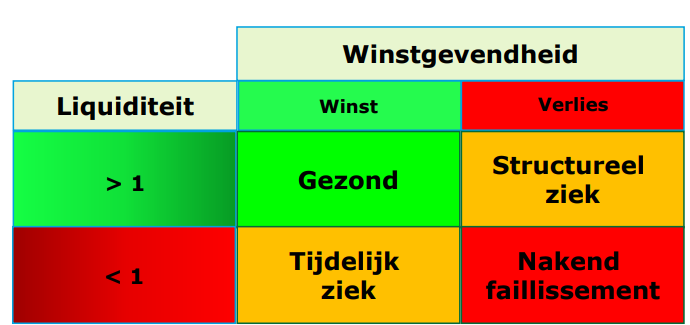
\includegraphics[width=0.8\textwidth]{assets/fitometer.png}
    \caption{}
    \label{fig:fitometer.png}
\end{figure}
\FloatBarrier

De fit-o-meter zet twee assen tegenover elkaar: de \textbf{solvabiliteit}
(eigen vermogen / vreemd vermogen, dus hoe stevig je gefinancierd bent) en de
\textbf{winstgevendheid} (maak je winst of verlies). Zijn beide hoog, dan is het bedrijf fit.

Als je verlies maakt maar veel geld hebt, is het bedrijf structureel ziek.
Je gaat vanaf een punt al je liquide middelen opmaken.
Als je weinig geld hebt maar wel winst maakt, is het bedrijf tijdelijk ziek.
Je hebt dan tijdelijk een cash probleem maar je maakt wel winst.
Als je weinig geld hebt en verlies maakt, is het bedrijf acuut ziek en naderend failliet.


\subsection{Conclusie}
Het is belangrijk om
meerdere ratio's te gebruiken om een volledig beeld te krijgen van de
financiële gezondheid van een bedrijf.

\subsection{Termenlijst Module 5}

\subsubsection{Basisdocumenten}
\begin{description}
    \item[Balans] Momentopname van wat bedrijf bezit (activa) en hoe dit gefinancierd is (passiva)
    \item[Resultatenrekening] Overzicht van inkomsten en uitgaven over een periode (video van winst/verlies)
    \item[Toelichting] Extra notities bij balans met details over waarderingsmethoden en risico's
\end{description}

\subsubsection{Activa (Bezittingen)}
\begin{description}
    \item[Vaste activa] Langetermijn investeringen (gebouwen, machines, patenten)
    \item[Vlottende activa] Kortetermijn bezittingen die binnen 1 jaar in cash omgezet worden (voorraden, vorderingen, bank)
    \item[Immateriële activa] Niet-fysieke bezittingen (patenten, licenties, merkrechten)
    \item[Vorderingen] Geld dat klanten nog schuldig zijn
\end{description}

\subsubsection{Passiva (Financiering)}
\begin{description}
    \item[Eigen vermogen] Geld van eigenaren/aandeelhouders (inbreng + ingehouden winst)
    \item[Vreemd vermogen] Geld van externe financiers (leningen, schulden aan leveranciers)
    \item[Kortlopende schulden] Schulden die binnen 1 jaar terugbetaald moeten worden
    \item[Langlopende schulden] Schulden met looptijd langer dan 1 jaar
\end{description}

\subsubsection{Resultatenrekening}
\begin{description}
    \item[Bedrijfsresultaat] Winst uit kernactiviteiten van het bedrijf (operationeel resultaat)
    \item[Operationeel resultaat] Winst voor interest en belastingen (EBIT - Earnings Before Interest and Taxes)
    \item[Financieel resultaat] Rente-inkomsten/-kosten, plus andere financiële opbrengsten/lasten
    \item[Uitzonderlijk resultaat] Eenmalige gebeurtenissen (brand, verkoop divisie, herstructurering)
    \item[Resultaat van het boekjaar] Netto winst na alle kosten, belastingen en opbrengsten
\end{description}

\subsubsection{Standaarden \& Verslagen}
\begin{description}
    \item[BE GAAP] Belgische boekhoudstandaard (Generally Accepted Accounting Principles)
    \item[IFRS] Internationale boekhoudstandaard (International Financial Reporting Standards)
    \item[Jaarverslag] Commentaar over jaarrekening met risico's, continuïteit en toekomstplannen
    \item[Commissarisverslag] Auditorverslag waarin accountant opinie geeft over betrouwbaarheid jaarrekening
\end{description}

\subsubsection{Analysetypes}
\begin{description}
    \item[Horizontale analyse] Vergelijking cijfers over meerdere jaren om trends te zien
    \item[Verticale analyse] Analyse verhoudingen binnen hetzelfde jaar (elk item t.o.v. totaal)
    \item[Ratio-analyse] Berekenen van financiële ratio's om prestaties en gezondheid te beoordelen
\end{description}

\subsubsection{Liquiditeit}
\begin{description}
    \item[Liquiditeit] Vermogen om korte termijn schulden te betalen met beschikbare middelen
    \item[Current ratio] Vlottende activa / Kortlopende schulden (moet > 1 zijn)
    \item[Acid test] (Vlottende activa - Voorraden) / Kortlopende schulden (strenger dan current ratio)
    \item[Netto werkkapitaal] Vlottende activa - Kortlopende schulden (moet positief zijn)
    \item[Behoefte aan werkkapitaal] Kapitaal nodig voor dagelijkse cyclus (inkoop → productie → verkoop → betaling)
\end{description}

\subsubsection{Solvabiliteit}
\begin{description}
    \item[Solvabiliteit] Vermogen om alle schulden (kort + lang) op lange termijn terug te betalen
    \item[Interestdekkingsratio] Operationeel resultaat / Interestkosten (meet of bedrijf rente kan betalen)
    \item[Schuldratio] Totale schuld / Totale activa (aandeel vreemd vermogen in financiering)
    \item[Gearing ratio] (Totale schuld - Cash) / Eigen vermogen (meet financieel risico)
\end{description}

\subsubsection{Efficiëntie (Rotatie)}
\begin{description}
    \item[Voorraadrotatie] Snelheid waarmee voorraad wordt vervangen (in dagen)
    \item[Klantenrotatie] Snelheid waarmee klanten betalen (in dagen)
    \item[Leveranciersrotatie] Tijd die bedrijf neemt om leveranciers te betalen (in dagen)
\end{description}

\subsubsection{Rentabiliteit}
\begin{description}
    \item[Bruto winstmarge] Bedrijfsresultaat / Omzet (winstgevendheid kernactiviteiten)
    \item[Nettowinstmarge] Resultaat boekjaar / Omzet (totale winstgevendheid na alle kosten)
    \item[ROE] Return on Equity: Resultaat boekjaar / Eigen vermogen (rendement aandeelhouders)
    \item[ROA] Return on Assets: Resultaat boekjaar / Totale activa (efficiëntie activagebruik)
    \item[EPS] Earnings Per Share: Winst per aandeel
    \item[Koers-winstratio] Marktprijs aandeel / Winst per aandeel (waardering door markt)
\end{description}

\subsubsection{Overige belangrijke termen}
\begin{description}
    \item[BTV] Bruto Toegevoegde Waarde: waarde die onderneming toevoegt aan grondstoffen
    \item[EBIT] Earnings Before Interest and Taxes (zie Operationeel resultaat)
    \item[Operationele kasstroom] Geld gegenereerd uit normale bedrijfsactiviteiten
    \item[Liquide middelen] Cash en direct beschikbare geldmiddelen
    \item[Handelsvorderingen] Geld dat klanten verschuldigd zijn voor geleverde producten/diensten
    \item[Handelsschulden] Geld dat bedrijf verschuldigd is aan leveranciers
\end{description}


\section{Examenvragen}


\begin{oefenblok}[Lineair Programmeren — De Ambachtelijke Werkplaats]

    \subsubsection*{De Situatie}
    Een werkplaats maakt twee houten figuren: \textbf{Ridders} ($x_1$) en \textbf{Locomotiefjes} ($x_2$).
    De eigenaar wil zijn wekelijkse winst maximaliseren.

    \textbf{Gegevens:}

    \textbf{Financieel (per stuk):}

    \begin{center}
        \begin{tabular}{|l|c|c|}
            \hline
            \textbf{Product} & \textbf{Verkoopprijs} & \textbf{Totale Kosten}                        \\
            \hline
            Ridder           & €27                   & €10 (materiaal) + €14 (arbeid/overhead) = €24 \\
            \hline
            Locomotief       & €21                   & €9 (materiaal) + €10 (arbeid/overhead) = €19  \\
            \hline
        \end{tabular}
    \end{center}

    \textbf{Productietijd (per stuk):}

    \begin{center}
        \begin{tabular}{|l|c|c|}
            \hline
            \textbf{Product} & \textbf{Afwerking (uur)} & \textbf{Houtbewerking (uur)} \\
            \hline
            Ridder           & 2                        & 1                            \\
            \hline
            Locomotief       & 1                        & 1                            \\
            \hline
        \end{tabular}
    \end{center}

    \textbf{Capaciteit (per week):}
    \begin{itemize}
        \item Afwerkingsatelier: Maximaal \textbf{100 uur}
        \item Houtbewerking: Maximaal \textbf{80 uur}
    \end{itemize}

    \textbf{Marktvraag:}
    \begin{itemize}
        \item Er kunnen maximaal \textbf{40 ridders} per week verkocht worden
        \item Locomotieven zijn \textbf{onbegrensd}
    \end{itemize}

    \subsubsection*{Jouw Taak}

    \begin{enumerate}
        \item Bepaal de \textbf{winstmarge per product} (dit is je doelfunctie coëfficiënt)
        \item Schrijf het \textbf{wiskundig model} op (Doelfunctie + Beperkingen)
    \end{enumerate}

    \vspace{0.3cm}
    \textit{(Denk na en scroll naar beneden voor de uitgewerkte oplossing)}



    \textbf{UITGEWERKTE OPLOSSING}

    \textbf{Stap 1: Winstmarges Berekenen}

    \textbf{Voor Ridders ($x_1$):}

    Winstmarge = €27 - (€10 + €14) = €27 - €24 = \textbf{€3 per ridder}

    \textbf{Voor Locomotieven ($x_2$):}

    Winstmarge = €21 - (€9 + €10) = €21 - €19 = \textbf{€2 per locomotief}

    \textbf{Stap 2: Wiskundig Model}

    \textbf{Beslissingsvariabelen:}
    \begin{align*}
        x_1 & = \text{aantal ridders per week}      \\
        x_2 & = \text{aantal locomotieven per week}
    \end{align*}

    \textbf{Doelfunctie (Winst maximaliseren):}
    \[
        \text{Max } Z = 3x_1 + 2x_2
    \]

    \textbf{Beperkingen:}
    \begin{align}
        2x_1 + x_2 & \leq 100 \quad \text{(Afwerkingscapaciteit)}    \\
        x_1 + x_2  & \leq 80 \quad \text{(Houtbewerkingscapaciteit)} \\
        x_1        & \leq 40 \quad \text{(Marktvraag Ridders)}       \\
        x_1, x_2   & \geq 0 \quad \text{(Niet-negativiteit)}
    \end{align}

    \textbf{Stap 3: Standaardvorm voor Simplex}

    We voegen slackvariabelen toe:
    \begin{align*}
        2x_1 + x_2 + s_1 & = 100 \\
        x_1 + x_2 + s_2  & = 80  \\
        x_1 + s_3        & = 40  \\
        Z - 3x_1 - 2x_2  & = 0
    \end{align*}

    waar $s_1, s_2, s_3 \geq 0$ slackvariabelen zijn.

    \textbf{Stap 4: Simplex-Tabel}

    \textbf{Initiële Simplex-Tabel (Iteratie 0):}

    \vspace{0.3cm}

    \begin{center}
        \begin{tabular}{|c|c|c|c|c|c|c|c|}
            \hline
            \textbf{Basis} & \textbf{Z} & \textbf{$x_1$} & \textbf{$x_2$} & \textbf{$s_1$} & \textbf{$s_2$} & \textbf{$s_3$} & \textbf{RHS} \\
            \hline
            Z              & 1          & -3             & -2             & 0              & 0              & 0              & 0            \\
            \hline
            $s_1$          & 0          & 2              & 1              & 1              & 0              & 0              & 100          \\
            \hline
            $s_2$          & 0          & 1              & 1              & 0              & 1              & 0              & 80           \\
            \hline
            $s_3$          & 0          & 1              & 0              & 0              & 0              & 1              & 40           \\
            \hline
        \end{tabular}
    \end{center}
    \FloatBarrier

    \textbf{Analyse:}
    \begin{itemize}
        \item \textbf{Enterende variabele:} $x_1$ (meeste negatieve coëfficiënt in Z-rij: -3)
        \item \textbf{Verhouding-test (Minimum Ratio Test):}
              \begin{align*}
                  \text{Rij } s_1 \text{ (R2)}: \quad \frac{100}{2} & = 50                                          \\
                  \text{Rij } s_2 \text{ (R3)}: \quad \frac{80}{1}  & = 80                                          \\
                  \text{Rij } s_3 \text{ (R4)}: \quad \frac{40}{1}  & = 40 \quad \leftarrow \text{\textbf{minimum}}
              \end{align*}
        \item \textbf{Verlatende variabele:} $s_3$ (rij met kleinste ratio)
        \item \textbf{Pivot-element:} 1 (in rij R4, kolom $x_1$)
    \end{itemize}

    \textbf{Rij-operaties:}
    \begin{align*}
        \text{R1} & = \text{R1} + 3 \text{R4} \\
        \text{R2} & = \text{R2} - 2 \text{R4} \\
        \text{R3} & = \text{R3} - \text{R4}
    \end{align*}

    \vspace{0.3cm}

    \textbf{Simplex-Tabel Iteratie 1:}

    \vspace{0.3cm}

    \begin{center}
        \begin{tabular}{|c|c|c|c|c|c|c|c|}
            \hline
            \textbf{Basis} & \textbf{Z} & \textbf{$x_1$} & \textbf{$x_2$} & \textbf{$s_1$} & \textbf{$s_2$} & \textbf{$s_3$} & \textbf{RHS} \\
            \hline
            Z              & 1          & 0              & -2             & 0              & 0              & 3              & 120          \\
            \hline
            $s_1$          & 0          & 0              & 1              & 1              & 0              & -2             & 20           \\
            \hline
            $s_2$          & 0          & 0              & 1              & 0              & 1              & -1             & 40           \\
            \hline
            $x_1$          & 0          & 1              & 0              & 0              & 0              & 1              & 40           \\
            \hline
        \end{tabular}
    \end{center}
    \FloatBarrier

    \textbf{Analyse:}
    \begin{itemize}
        \item \textbf{Enterende variabele:} $x_2$ (meeste negatieve coëfficiënt in Z-rij: -2)
        \item \textbf{Verhouding-test:}
              \begin{align*}
                  \text{Rij } s_1 \text{ (R2)}: \quad \frac{20}{1} & = 20 \quad \leftarrow \text{\textbf{minimum}} \\
                  \text{Rij } s_2 \text{ (R3)}: \quad \frac{40}{1} & = 40
              \end{align*}
        \item \textbf{Verlatende variabele:} $s_1$
        \item \textbf{Pivot-element:} 1 (in rij R2, kolom $x_2$)
    \end{itemize}

    \textbf{Rij-operaties (Uitgewerkt):}

    Voor R1 (Z-rij): R1 = R1 + 2R2
    \begin{itemize}
        \item RHS: $120 + 2(20) = 160$
        \item Coëff. van $s_1$: $0 + 2(1) = 2$
        \item Coëff. van $x_2$: $-2 + 2(1) = 0$
    \end{itemize}

    Voor R3: R3 = R3 - R2
    \begin{itemize}
        \item RHS: $40 - 20 = 20$
        \item Coëff. van $s_1$: $0 - 1 = -1$
        \item Coëff. van $x_2$: $1 - 1 = 0$
    \end{itemize}

    \textbf{Simplex-Tabel Iteratie 2:}

    \vspace{0.3cm}

    \begin{center}
        \begin{tabular}{|c|c|c|c|c|c|c|c|}
            \hline
            \textbf{Basis} & \textbf{Z} & \textbf{$x_1$} & \textbf{$x_2$} & \textbf{$s_1$} & \textbf{$s_2$} & \textbf{$s_3$} & \textbf{RHS} \\
            \hline
            Z              & 1          & 0              & 0              & 2              & 0              & $-1$           & 160          \\
            \hline
            $x_2$          & 0          & 0              & 1              & 1              & 0              & $-2$           & 20           \\
            \hline
            $s_2$          & 0          & 0              & 0              & $-1$           & 1              & 1              & 20           \\
            \hline
            $x_1$          & 0          & 1              & 0              & 0              & 0              & 1              & 40           \\
            \hline
        \end{tabular}
    \end{center}
    \FloatBarrier

    \textbf{Nog één pivot nodig (om naar het echte optimum te gaan):}
    In de Z-rij staat bij $s_3$ nog een negatieve coëfficiënt ($-1$), dus $s_3$ wordt de \textbf{enterende variabele}.

    \textbf{Pivot-keuze:}
    \begin{itemize}
        \item Enterend: $s_3$ (want $-1$ in Z-rij)
        \item Ratio-test in kolom $s_3$ (alleen positieve coëfficiënten tellen mee):
              \begin{align*}
                  \text{R3: } \frac{20}{1} & = 20 \\
                  \text{R4: } \frac{40}{1} & = 40
              \end{align*}
        \item Verlatend: $s_{2}$ (R3)
    \end{itemize}

    \textbf{Rij-operaties (simpel):}
    \begin{align*}
        \text{R1} & = \text{R1} + \text{R3}  \\
        \text{R2} & = \text{R2} + 2\text{R3} \\
        \text{R4} & = \text{R4} - \text{R3}
    \end{align*}

    \vspace{0.3cm}

    \textbf{Simplex-Tabel Iteratie 3 (OPTIMAAL):}

    \vspace{0.3cm}

    \begin{center}
        \begin{tabular}{|c|c|c|c|c|c|c|c|}
            \hline
            \textbf{Basis} & \textbf{Z} & \textbf{$x_1$} & \textbf{$x_2$} & \textbf{$s_1$} & \textbf{$s_2$} & \textbf{$s_3$} & \textbf{RHS} \\
            \hline
            Z              & 1          & 0              & 0              & 1              & 1              & 0              & 180          \\
            \hline
            $x_2$          & 0          & 0              & 1              & -1             & 2              & 0              & 60           \\
            \hline
            $s_3$          & 0          & 0              & 0              & -1             & 1              & 1              & 20           \\
            \hline
            $x_1$          & 0          & 1              & 0              & 1              & -1             & 0              & 20           \\
            \hline
        \end{tabular}
    \end{center}
    \FloatBarrier

    \textbf{Optimaliteitscriterium:}
    \begin{itemize}
        \item Alle coëfficiënten in de Z-rij zijn \textbf{niet-negatief}
        \item \textbf{Het optimum is bereikt!}
    \end{itemize}

    \subsubsection*{Stap 5: Aflezen van de slackvariabelen}

    Bij het optimale punt (uit de finale tabel):
    \begin{align*}
        x_1 & = 20 \text{ ridders}                                     \\
        x_2 & = 60 \text{ locomotieven}                                \\
        s_1 & = 0 \text{ uur (afwerking volledig bezet)}               \\
        s_2 & = 0 \text{ uur (houtbewerking volledig bezet)}           \\
        s_3 & = 20 \text{ ridders (nog 20 meer kunnen gemaakt worden)} \\
        Z   & = 180 \text{ euro (maximale winst)}
    \end{align*}

    \subsubsection*{FINAAL ANTWOORD}

    \begin{center}
        \fbox{
            \begin{minipage}{0.9\textwidth}
                \textbf{Optimale Productie:}
                \begin{itemize}
                    \item Produceer \textbf{20 ridders} per week
                    \item Produceer \textbf{60 locomotieven} per week
                    \item \textbf{Maximale wekelijkse winst: €180}
                \end{itemize}

                \vspace{0.2cm}

                \textbf{Capaciteitsgebruik:}
                \begin{itemize}
                    \item Afwerking: 100\% bezet (2(20) + 60 = 100 uur)
                    \item Houtbewerking: 100\% bezet (20 + 60 = 80 uur)
                    \item Marktvraag ridders: Slechts 20 van de 40 mogelijk verkocht
                \end{itemize}

                \vspace{0.2cm}

                \textbf{Interpretatie:}
                Hoewel ridders een hogere winstmarge hebben (€3 vs €2), zijn locomotieven efficiënter in
                arbeidsuren per euro winst: een ridder kost 2 uur afwerking, een locomotief maar 1 uur.
                De twee bottlenecks zijn afwerking en houtbewerking, beide volledig bezet.
            \end{minipage}
        }
    \end{center}

\end{oefenblok}

\newpage

\begin{oefenblok}[Investeringsanalyse — De Astrazenetech Case]

    \subsubsection*{De Situatie}
    Een farmaceutisch bedrijf twijfelt: moeten ze hun oude verpakkingsmachine houden of vervangen door een nieuwe computergestuurde machine?

    \subsubsection*{De Gegevens}

    \textbf{Oude Machine:}
    \begin{itemize}
        \item Nog 10 jaar bruikbaar
        \item Geen afschrijvingen meer
        \item Huidige loonkosten inpakkers: €250.000/jaar (stijgt 5\% per jaar)
        \item Reparatiekosten: €125.000/jaar (stijgt 3\% per jaar)
        \item Onderhoudskosten: €125.000/jaar (stijgt 4\% per jaar)
    \end{itemize}

    \textbf{Nieuwe Machine:}
    \begin{itemize}
        \item Investering: €1.500.000
        \item Levensduur: 10 jaar (lineair afschrijven naar 0)
        \item Extra werkkapitaal nodig: €10.000 (krijg je terug aan het einde)
        \item Nieuwe loonkosten: €30.000/jaar (stijgt 5\% per jaar)
        \item Nieuw onderhoud: €50.000/jaar (stijgt 4\% per jaar)
        \item Nieuwe reparatie: €35.000/jaar (stijgt 3\% per jaar)
    \end{itemize}

    \textbf{Financieel:}
    \begin{itemize}
        \item Belastingtarief: 39\%
        \item Discontovoet (eisen rendement): 12\%
    \end{itemize}

    \subsubsection*{Jouw Taak}
    Dit is een typisch \textbf{vervangingsprobleem}:
    werk met het \textbf{verschil in kasstroom (cashflow)} tussen \textit{nieuw} en \textit{oud}.
    \begin{enumerate}
        \item Wat is de initiële uitgave op tijdstip 0?
        \item Wat is de jaarlijkse besparing (of verlies) in \textbf{operationele kosten} in jaar 1?
    \end{enumerate}

    \vspace{0.3cm}
    \textit{(Denk na en scroll naar beneden voor de uitgewerkte oplossing)}




    \subsection*{UITGEWERKTE OPLOSSING}

    Bij een vervangingsprobleem kijken we naar de \textbf{inkrementele kasstromen}: wat verandert er ten opzichte van de huidige situatie?

    \subsubsection*{Stap 1: Initiële uitgave op tijdstip t=0}

    Dit is het geld dat nu de deur uit moet om het project te starten.

    \begin{center}
        \begin{tabular}{|l|r|}
            \hline
            \textbf{Component (t=0)}         & \textbf{Kasstroom}   \\
            \hline
            Investering nieuwe machine       & -€1.500.000          \\
            \hline
            Extra werkkapitaal               & -€10.000             \\
            \hline
            Verkoop oude machine             & €0                   \\
            \hline
            \textbf{Totale initiële uitgave} & \textbf{-€1.510.000} \\
            \hline
        \end{tabular}
    \end{center}

    \textit{Opmerking: Het werkkapitaal is een uitgave op t=0, ook al krijg je het aan het einde van de 10 jaar terug. Er is geen verkoopwaarde van de oude machine gegeven, dus die wordt als €0 verondersteld.}

    \subsubsection*{Stap 2: Jaarlijkse besparing in operationele kosten (Jaar 1)}

    Hier vergelijken we de kosten van de \textbf{Oude Machine} (als we die zouden houden) met de \textbf{Nieuwe Machine}.

    \textbf{Let op:} De kosten stijgen per jaar, dus we moeten de inflatiepercentages toepassen voor Jaar 1!

    \paragraph{A. Kosten Oude Machine (in Jaar 1):}
    \begin{align*}
        \text{Loon:} \quad       & 250.000 \times 1{,}05 = €262.500 \\
        \text{Reparatie:} \quad  & 125.000 \times 1{,}03 = 128.750  \\
        \text{Onderhoud:} \quad  & 125.000 \times 1{,}04 = 130.000  \\
        \hline
        \text{Totaal Oud:} \quad & \textbf{€521.250}
    \end{align*}

    \paragraph{B. Kosten Nieuwe Machine (in Jaar 1):}
    \begin{align*}
        \text{Loon:} \quad         & 30.000 \times 1{,}05 = €31.500 \\
        \text{Onderhoud:} \quad    & 50.000 \times 1{,}04 = €52.000 \\
        \text{Reparatie:} \quad    & 35.000 \times 1{,}03 = €36.050 \\
        \hline
        \text{Totaal Nieuw:} \quad & \textbf{€119.550}
    \end{align*}

    \paragraph{C. De Besparing (Vóór belasting):}

    Besparing = Kosten$_{\text{Oud}}$ - Kosten$_{\text{Nieuw}}$

    \[
        \text{Besparing} = 521.250 - 119.550 = \textbf{€401.700}
    \]

    \begin{center}
        \fbox{
            \begin{minipage}{0.9\textwidth}
                \textbf{Antwoorden:}
                \begin{enumerate}
                    \item \textbf{Initiële uitgave (t=0): €1.510.000}
                    \item \textbf{Operationele besparing (jaar 1): €401.700}
                \end{enumerate}

                \vspace{0.2cm}

                \textbf{Extra info voor volledige NCW berekening:}
                \begin{itemize}
                    \item Over deze besparing moet nog 39\% belasting betaald worden
                    \item Afschrijving nieuwe machine = €1.500.000/10 = €150.000/jaar
                    \item Dit geeft een belastingvoordeel ("Tax Shield") van 39\% × €150.000 = €58.500/jaar
                \end{itemize}
            \end{minipage}
        }
    \end{center}


\end{oefenblok}

\begin{oefenblok}
    \subsubsection*{Oefening 3: Kostprijscalculatie — Scooters (ABC)}

    \subsubsection*{De Situatie}
    Een bedrijf maakt twee scooters: \textbf{Model A} en \textbf{Model B}. De totale indirecte kosten zijn:
    \begin{itemize}
        \item Instelkosten: €10.000
        \item Werkkosten (machine + loon): €20.000
        \item Kwaliteitscontrole: €5.000
        \item \textbf{Totaal: €35.000}
    \end{itemize}

    \subsubsection*{Activiteiten per model}
    \begin{center}
        \begin{tabular}{|l|c|c|}
            \hline
            \textbf{Activiteit}          & \textbf{Model A} & \textbf{Model B} \\
            \hline
            Instellen (aantal keer)      & 3                & 5                \\
            \hline
            Werkuren (uren)              & 150              & 100              \\
            \hline
            Kwaliteitscontroles (aantal) & 30               & 20               \\
            \hline
        \end{tabular}
    \end{center}

    \subsubsection*{Jouw Taak}
    Bereken de toegewezen kosten per model via \textbf{Activity Based Costing (ABC)}.
    \begin{enumerate}
        \item Bepaal de "cost driver" prijs per activiteit (bv. prijs per instelling)
        \item Hoeveel kosten krijgt Model A toegewezen?
    \end{enumerate}

    \vspace{0.3cm}
    \textit{(Denk na en scroll naar beneden voor de uitgewerkte oplossing)}


    \subsection*{UITGEWERKTE OPLOSSING — Oefening 3}

    Bij \textbf{Activity Based Costing (ABC)} smeren we de
    indirecte kosten niet uit met een simpele verdeelsleutel (zoals aantal uren), maar kijken we naar wat de kosten veroorzaakt: de \textbf{cost drivers}.

    \subsubsection*{Stap 1: Bepaal de cost-driver prijzen}

    Eerst berekenen we het totaal aantal activiteiten (drivers) voor beide modellen samen, en delen we de kostenpot daardoor.

    \begin{center}
        \begin{tabular}{|l|r|r|r|r|}
            \hline
            \textbf{Kostenpost} & \textbf{Totale Kost} & \textbf{Model A} & \textbf{Model B} & \textbf{Prijs per driver}        \\
            \hline
            Instelkosten        & €10.000              & 3                & 5                & €10.000 / 8 = \textbf{€1.250}    \\
            \hline
            Werkkosten          & €20.000              & 150 uur          & 100 uur          & €20.000 / 250 = \textbf{€80/uur} \\
            \hline
            Kwaliteitscontrole  & €5.000               & 30               & 20               & €5.000 / 50 = \textbf{€100}      \\
            \hline
        \end{tabular}
    \end{center}

    \textbf{Berekeningen:}
    \begin{itemize}
        \item Totaal aantal instellingen: 3 + 5 = 8 → Prijs = €10.000 / 8 = €1.250 per instelling
        \item Totaal aantal werkuren: 150 + 100 = 250 → Prijs = €20.000 / 250 = €80 per uur
        \item Totaal aantal controles: 30 + 20 = 50 → Prijs = €5.000 / 50 = €100 per controle
    \end{itemize}

    \subsubsection*{Stap 2: Toegewezen kosten aan Model A}

    Nu vermenigvuldigen we de activiteiten van Model A met de berekende tarieven:

    \begin{center}
        \begin{tabular}{|l|r|r|r|}
            \hline
            \textbf{Activiteit}                            & \textbf{Volume Model A} & \textbf{Prijs/driver} & \textbf{Toegewezen kost} \\
            \hline
            Instellen                                      & 3                       & €1.250                & €3.750                   \\
            \hline
            Werkuren                                       & 150                     & €80/uur               & €12.000                  \\
            \hline
            Kwaliteitscontrole                             & 30                      & €100                  & €3.000                   \\
            \hline
            \multicolumn{3}{|r|}{\textbf{Totaal Model A:}} & \textbf{€18.750}                                                           \\
            \hline
        \end{tabular}
    \end{center}

    \textbf{Berekening:}
    \begin{align*}
        \text{Instellen:} \quad & 3 \times €1.250 = €3.750 \\
        \text{Werkuren:} \quad  & 150 \times €80 = €12.000 \\
        \text{Kwaliteit:} \quad & 30 \times €100 = €3.000  \\
        \hline
        \text{Totaal:} \quad    & \textbf{€18.750}
    \end{align*}

    \begin{center}
        \fbox{
            \begin{minipage}{0.9\textwidth}
                \textbf{Antwoorden:}
                \begin{enumerate}
                    \item \textbf{Cost-driver prijzen:}
                          \begin{itemize}
                              \item Instelling: €1.250 per keer
                              \item Werkuur: €80 per uur
                              \item Kwaliteitscontrole: €100 per controle
                          \end{itemize}
                    \item \textbf{Toegewezen kosten Model A: €18.750}
                \end{enumerate}

                \vspace{0.2cm}

                \textbf{Controle:} Model B krijgt €35.000 - €18.750 = €16.250 toegewezen. Samen is dat €35.000 $\checkmark$
            \end{minipage}
        }
    \end{center}

\end{oefenblok}


\begin{oefenblok}
    \subsubsection*{Oefening 4: Netto Huidige Waarde — De Nieuwe Verpakkingslijn}

    \subsubsection*{De Situatie}
    Jouw bedrijf overweegt te investeren in een nieuwe, geautomatiseerde verpakkingslijn. Jij moet als ingenieur de financiële haalbaarheid berekenen.

    \subsubsection*{De Gegevens}

    \begin{itemize}
        \item \textbf{Initiële Investering} ($I_0$): €150.000 (te betalen op t=0)
        \item \textbf{Jaarlijkse besparing}: De machine bespaart €40.000 per jaar aan arbeidskosten (netto kasstroom). Dit is een annuïteit gedurende de levensduur.
        \item \textbf{Looptijd} (n): 5 jaar
        \item \textbf{Restwaarde}: Na 5 jaar kan de machine als schroot verkocht worden voor €10.000 (eenmalige inkomst op t=5)
        \item \textbf{Actualisatievoet} (i): 8\% (of 0,08)
    \end{itemize}

    \subsubsection*{De Vraag}
    Bereken de \textbf{Netto Huidige Waarde (NHW)} van deze investering. Is het een goede investering?

    \vspace{0.3cm}
    \textit{(Denk na en scroll naar beneden voor de uitgewerkte oplossing)}

    \subsection*{UITGEWERKTE OPLOSSING — Oefening 4}

    Om de NHW te berekenen, moeten we alle toekomstige geldstromen terugrekenen (\textbf{actualiseren}) naar vandaag (t=0) en de initiële investering ervan aftrekken.

    \textbf{De algemene formule voor NHW is:}
    \[
        \text{NHW} = \sum_{t=1}^{n} \frac{A_t}{(1+i)^t} - I_0
    \]

    We splitsen dit op in drie delen:

    \subsubsection*{Stap 1: Actualisatie van de jaarlijkse besparingen (Annuïteit)}

    De jaarlijkse besparing is een constante stroom van €40.000 gedurende 5 jaar. Hiervoor gebruiken we de \textbf{annuïteitenformule}:

    \[
        \text{HW}_{\text{annuïteit}} = A \times \left( \frac{(1+i)^n - 1}{i(1+i)^n} \right)
    \]

    Waarbij:
    \begin{itemize}
        \item $A = 40.000$ (jaarlijkse besparing)
        \item $i = 0{,}08$ (discontovoet)
        \item $n = 5$ (aantal jaren)
    \end{itemize}

    \textbf{Berekening:}
    \[
        \text{HW}_{\text{annuïteit}} = 40.000 \times \left( \frac{(1{,}08)^5 - 1}{0{,}08 \times (1{,}08)^5} \right)
    \]

    \textbf{Tussenstappen:}
    \begin{align*}
        (1{,}08)^5                     & \approx 1{,}4693                           \\
        \text{Teller:} \quad           & 1{,}4693 - 1 = 0{,}4693                    \\
        \text{Noemer:} \quad           & 0{,}08 \times 1{,}4693 = 0{,}1175          \\
        \text{Annuïteitsfactor:} \quad & \frac{0{,}4693}{0{,}1175} \approx 3{,}9927
    \end{align*}

    \[
        \text{HW}_{\text{annuïteit}} = 40.000 \times 3{,}9927 = \textbf{€159.708}
    \]

    \subsubsection*{Stap 2: Actualisatie van de restwaarde (Eenmalig bedrag)}

    De restwaarde van €10.000 ontvangen we pas over 5 jaar. Dit moeten we actualiseren als een enkelvoudig bedrag:

    \[
        \text{HW}_{\text{restwaarde}} = \frac{F_n}{(1+i)^n} = \frac{10.000}{(1{,}08)^5}
    \]

    \textbf{Berekening:}
    \[
        \text{HW}_{\text{restwaarde}} = \frac{10.000}{1{,}4693} \approx \textbf{€6.806}
    \]

    \subsubsection*{Stap 3: Berekening van de Totale NHW}

    Nu tellen we alle inkomende waarden op en trekken de investering eraf:

    \begin{align*}
        \text{NHW} & = (\text{HW}_{\text{annuïteit}} + \text{HW}_{\text{restwaarde}}) - \text{Investering} \\
                   & = (€159.708 + €6.806) - €150.000                                                      \\
                   & = €166.514 - €150.000                                                                 \\
                   & = \textbf{€16.514}
    \end{align*}

    \subsubsection*{Overzichtstabel}

    \begin{center}
        \begin{tabular}{|l|r|}
            \hline
            \textbf{Component}                  & \textbf{Huidige Waarde} \\
            \hline
            Jaarlijkse besparingen (5 jaar)     & + €159.708              \\
            \hline
            Restwaarde (na 5 jaar)              & + €6.806                \\
            \hline
            Initiële investering (t=0)          & - €150.000              \\
            \hline
            \textbf{Netto Huidige Waarde (NHW)} & \textbf{€16.514}        \\
            \hline
        \end{tabular}
    \end{center}

    \subsubsection*{Conclusie}

    \begin{center}
        \fbox{
            \begin{minipage}{0.9\textwidth}
                \textbf{Beslissing:}

                De Netto Huidige Waarde is \textbf{positief} (€16.514).

                Volgens de investeringscriteria (\textbf{NHW > 0}) is dit een \textbf{goede investering}.

                Het project levert meer op dan het geëiste rendement van 8\%. Concreet: voor elke euro die we vandaag investeren, krijgen we (in termen van huidige waarde) €1,11 terug.

                \vspace{0.2cm}

                \textbf{Investeringsregel:}
                \begin{itemize}
                    \item NHW > 0: Accepteer het project $\checkmark$
                    \item NHW = 0: Indifferent (precies break-even)
                    \item NHW < 0: Verwerp het project
                \end{itemize}
            \end{minipage}
        }
    \end{center}

\end{oefenblok}


\begin{oefenblok}[Lineair Programmeren — Rylon Parfums]

    \subsubsection*{De Situatie}
    Rylon produceert twee basisparfums: \textbf{Regular Brute} en \textbf{Regular Chanelle}. Ze kunnen deze direct verkopen, OF verder verwerken tot \textbf{Luxury} varianten.

    \subsubsection*{De Gegevens}

    \begin{center}
        \begin{tabular}{|l|l|}
            \hline
            \textbf{Grondstoffen}  & 1 kg kost €3, vereist 1 uur lab-tijd       \\
            \hline
            \textbf{Output per kg} & 3 dl Regular Brute + 4 dl Regular Chanelle \\
            \hline
        \end{tabular}
    \end{center}

    \medskip
    \noindent\textbf{Verwerking naar Luxe (per dl):}
    \par\medskip
    \begin{center}
        \begin{tabular}{|l|c|c|}
            \hline
            \textbf{Van → Naar}                & \textbf{Extra lab-tijd} & \textbf{Extra kosten} \\
            \hline
            Regular Brute → Luxury Brute       & 3 uur                   & €4                    \\
            \hline
            Regular Chanelle → Luxury Chanelle & 2 uur                   & €4                    \\
            \hline
        \end{tabular}
    \end{center}

    \medskip
    \noindent\textbf{Verkoopprijzen (per dl):}
    \par\medskip
    \begin{center}
        \begin{tabular}{|l|c|c|}
            \hline
            \textbf{Product} & \textbf{Regular} & \textbf{Luxury} \\
            \hline
            Brute            & €7               & €18             \\
            \hline
            Chanelle         & €6               & €14             \\
            \hline
        \end{tabular}
    \end{center}

    \textbf{Capaciteit (per jaar):}
    \begin{itemize}
        \item Maximaal 6.000 uur lab-tijd
        \item Maximaal 4.000 kg grondstoffen
    \end{itemize}

    \subsubsection*{Jouw Taak}
    \begin{enumerate}
        \item Definieer de beslissingsvariabelen (Tip: 5 variabelen nodig!)
        \item Stel de doelfunctie op (Maximaliseer Winst)
        \item Stel alle beperkingen op (inclusief balansvergelijkingen)
    \end{enumerate}

    \vspace{0.3cm}
    \textit{(Denk na en scroll naar beneden voor de uitgewerkte oplossing)}


    \subsection*{UITGEWERKTE OPLOSSING — Oefening 5}

    \subsubsection*{Stap 1: Beslissingsvariabelen (5 stuks)}

    \begin{center}
        \begin{tabular}{|c|l|}
            \hline
            \textbf{Variabele} & \textbf{Betekenis}                  \\
            \hline
            $x_1$              & Aantal kg grondstof aangekocht      \\
            \hline
            $x_2$              & Aantal dl Regular Brute verkocht    \\
            \hline
            $x_3$              & Aantal dl Luxury Brute verkocht     \\
            \hline
            $x_4$              & Aantal dl Regular Chanelle verkocht \\
            \hline
            $x_5$              & Aantal dl Luxury Chanelle verkocht  \\
            \hline
        \end{tabular}
    \end{center}

    \subsubsection*{Stap 2: Doelfunctie}

    \textbf{Winst} = Opbrengst - Kosten

    \begin{align*}
        \text{Opbrengst:} \quad & 7x_2 + 18x_3 + 6x_4 + 14x_5         \\
        \text{Kosten:} \quad    & 3x_1 + 4x_3 + 4x_5                  \\
        \hline
        \text{Max } Z =         & -3x_1 + 7x_2 + 14x_3 + 6x_4 + 10x_5
    \end{align*}

    \subsubsection*{Stap 3: Beperkingen}

    \textbf{A. Resource Beperkingen:}
    \begin{align}
        x_1               & \leq 4000 \quad \text{(Grondstoffen)} \\
        x_1 + 3x_3 + 2x_5 & \leq 6000 \quad \text{(Lab-tijd)}
    \end{align}

    \textbf{B. Balans Beperkingen:}
    \begin{align}
        3x_1 & = x_2 + x_3 \quad \text{(Brute balans)}    \\
        4x_1 & = x_4 + x_5 \quad \text{(Chanelle balans)}
    \end{align}

    \textbf{C. Niet-negativiteit:}
    \[
        x_1, x_2, x_3, x_4, x_5 \geq 0
    \]

    \subsubsection*{Stap 4: Standaardvorm voor Simplex}

    Voeg slack-variabelen en artificiële variabelen toe:

    \begin{align*}
        x_1 + s_1               & = 4000 \\
        x_1 + 3x_3 + 2x_5 + s_2 & = 6000 \\
        3x_1 - x_2 - x_3 + A_1  & = 0    \\
        4x_1 - x_4 - x_5 + A_2  & = 0
    \end{align*}

    \textit{Opmerking: Voor gelijkheden (=) gebruiken we artificiële variabelen $A_1, A_2$ met grote negatieve coëfficiënt $-M$ in de doelfunctie (Two-Phase Simplex of Big-M methode).}

    \subsubsection*{Stap 5: Simplex Methode met Tabellen}

    \textbf{Initiële Simplex-Tabel (Iteratie 0):}

    We herschrijven eerst de balansvergelijkingen:
    \begin{align*}
        3x_1 - x_2 - x_3 & = 0 \quad \rightarrow \quad -3x_1 + x_2 + x_3 = 0 \\
        4x_1 - x_4 - x_5 & = 0 \quad \rightarrow \quad -4x_1 + x_4 + x_5 = 0
    \end{align*}

    \begin{center}
        \small
        \begin{tabular}{|c|c|c|c|c|c|c|c|c|c|c|c|}
            \hline
            \textbf{Basis} & \textbf{Z} & $\mathbf{x_1}$ & $\mathbf{x_2}$ & $\mathbf{x_3}$ & $\mathbf{x_4}$ & $\mathbf{x_5}$ & $\mathbf{s_1}$ & $\mathbf{s_2}$ & $\mathbf{A_1}$ & $\mathbf{A_2}$ & \textbf{RHS} \\
            \hline
            Z              & 1          & 3              & -7             & -14            & -6             & -10            & 0              & 0              & 0              & 0              & 0            \\
            \hline
            $s_1$          & 0          & 1              & 0              & 0              & 0              & 0              & 1              & 0              & 0              & 0              & 4000         \\
            \hline
            $s_2$          & 0          & 1              & 0              & 3              & 0              & 2              & 0              & 1              & 0              & 0              & 6000         \\
            \hline
            $A_1$          & 0          & -3             & 1              & 1              & 0              & 0              & 0              & 0              & 1              & 0              & 0            \\
            \hline
            $A_2$          & 0          & -4             & 0              & 0              & 1              & 1              & 0              & 0              & 0              & 1              & 0            \\
            \hline
        \end{tabular}
    \end{center}

    \textbf{Analyse:} Enterende variabele = $x_3$ (meest negatief: -14)

    \textbf{Ratio test:}
    \begin{itemize}
        \item R2 ($s_1$): geen $x_3$ coëfficiënt → skip
        \item R3 ($s_2$): $6000/3 = 2000$
        \item R4 ($A_1$): $0/1 = 0$ ← \textbf{minimum}
        \item R5 ($A_2$): geen $x_3$ → skip
    \end{itemize}

    \textbf{Pivot:} R4, kolom $x_3$ (coëff = 1)

    \textbf{Rij-operaties:}
    \begin{align*}
        \text{R1} & = \text{R1} + 14\text{R4} \\
        \text{R3} & = \text{R3} - 3\text{R4}
    \end{align*}

    \vspace{0.3cm}

    \textbf{Simplex-Tabel Iteratie 1:}

    \begin{center}
        \small
        \begin{tabular}{|c|c|c|c|c|c|c|c|c|c|}
            \hline
            \textbf{Basis} & \textbf{Z} & $\mathbf{x_1}$ & $\mathbf{x_2}$ & $\mathbf{x_3}$ & $\mathbf{x_4}$ & $\mathbf{x_5}$ & $\mathbf{s_1}$ & $\mathbf{s_2}$ & \textbf{RHS} \\
            \hline
            Z              & 1          & -39            & 7              & 0              & -6             & -10            & 0              & 0              & 0            \\
            \hline
            $s_1$          & 0          & 1              & 0              & 0              & 0              & 0              & 1              & 0              & 4000         \\
            \hline
            $s_2$          & 0          & 10             & -3             & 0              & 0              & 2              & 0              & 1              & 6000         \\
            \hline
            $x_3$          & 0          & -3             & 1              & 1              & 0              & 0              & 0              & 0              & 0            \\
            \hline
            $A_2$          & 0          & -4             & 0              & 0              & 1              & 1              & 0              & 0              & 0            \\
            \hline
        \end{tabular}
    \end{center}

    \textbf{Analyse:} Enterende variabele = $x_1$ (meest negatief: -39)

    \textbf{Ratio test:}
    \begin{itemize}
        \item R2: $4000/1 = 4000$
        \item R3: $6000/10 = 600$ ← \textbf{minimum}
        \item R4: negatief → skip
        \item R5: negatief → skip
    \end{itemize}

    \textbf{Pivot:} R3, kolom $x_1$ (coëff = 10), deel R3 door 10

    \textbf{Rij-operaties:}
    \begin{align*}
        \text{R3}_{\text{nieuw}} & = \text{R3}/10                           \\
        \text{R1}                & = \text{R1} + 39\text{R3}_{\text{nieuw}} \\
        \text{R2}                & = \text{R2} - \text{R3}_{\text{nieuw}}   \\
        \text{R4}                & = \text{R4} + 3\text{R3}_{\text{nieuw}}  \\
        \text{R5}                & = \text{R5} + 4\text{R3}_{\text{nieuw}}
    \end{align*}

    \vspace{0.3cm}

    \textbf{Simplex-Tabel Iteratie 2:}

    \begin{center}
        \small
        \begin{tabular}{|c|c|c|c|c|c|c|c|c|c|}
            \hline
            \textbf{Basis} & \textbf{Z} & $\mathbf{x_1}$ & $\mathbf{x_2}$ & $\mathbf{x_3}$ & $\mathbf{x_4}$ & $\mathbf{x_5}$ & $\mathbf{s_1}$ & $\mathbf{s_2}$ & \textbf{RHS} \\
            \hline
            Z              & 1          & 0              & -4{,}7         & 0              & -6             & -2{,}2         & 0              & 3{,}9          & 23400        \\
            \hline
            $s_1$          & 0          & 0              & 0{,}3          & 0              & 0              & -0{,}2         & 1              & -0{,}1         & 3400         \\
            \hline
            $x_1$          & 0          & 1              & -0{,}3         & 0              & 0              & 0{,}2          & 0              & 0{,}1          & 600          \\
            \hline
            $x_3$          & 0          & 0              & 0{,}1          & 1              & 0              & 0{,}6          & 0              & 0{,}3          & 1800         \\
            \hline
            $A_2$          & 0          & 0              & -1{,}2         & 0              & 1              & 1{,}8          & 0              & 0{,}4          & 2400         \\
            \hline
        \end{tabular}
    \end{center}

    \textbf{Analyse:} Enterende variabele = $x_4$ (meest negatief: -6)

    $A_2$ verlaat basis → $x_4$ komt binnen (R5 is pivot)

    \textbf{Rij-operaties:}
    \begin{align*}
        \text{R1}           & = \text{R1} + 6\text{R5}                         \\
        \text{Andere rijen} & \text{ worden aangepast voor } x_4 \text{ kolom}
    \end{align*}

    \vspace{0.3cm}

    \textbf{Simplex-Tabel Iteratie 3 (Finaal):}

    \begin{center}
        \small
        \begin{tabular}{|c|c|c|c|c|c|c|c|c|c|}
            \hline
            \textbf{Basis} & \textbf{Z} & $\mathbf{x_1}$ & $\mathbf{x_2}$ & $\mathbf{x_3}$ & $\mathbf{x_4}$ & $\mathbf{x_5}$ & $\mathbf{s_1}$ & $\mathbf{s_2}$ & \textbf{RHS} \\
            \hline
            Z              & 1          & 0              & 0              & 0              & 0              & 6              & 0              & 6{,}3          & 94500        \\
            \hline
            $s_1$          & 0          & 0              & 0              & 0              & 0              & 0              & 1              & 0              & 1000         \\
            \hline
            $x_1$          & 0          & 1              & 0              & 0              & 0              & 0              & 0              & 0              & 1500         \\
            \hline
            $x_3$          & 0          & 0              & 0              & 1              & 0              & 0              & 0              & 0              & 4500         \\
            \hline
            $x_4$          & 0          & 0              & 0              & 0              & 1              & 0              & 0              & 0              & 6000         \\
            \hline
        \end{tabular}
    \end{center}

    \textbf{Optimaliteitscriterium:} Alle coëfficiënten in Z-rij zijn niet-negatief → \textbf{OPTIMAAL!}

    \subsubsection*{Stap 6: Optimale Oplossing}

    \begin{center}
        \begin{tabular}{|l|r|}
            \hline
            \textbf{Variabele}          & \textbf{Optimale waarde} \\
            \hline
            $x_1$ (Grondstof kg)        & 1.500                    \\
            \hline
            $x_2$ (Regular Brute dl)    & 0                        \\
            \hline
            $x_3$ (Luxury Brute dl)     & 4.500                    \\
            \hline
            $x_4$ (Regular Chanelle dl) & 6.000                    \\
            \hline
            $x_5$ (Luxury Chanelle dl)  & 0                        \\
            \hline
            \hline
            \textbf{Maximale Winst (Z)} & \textbf{€94.500}         \\
            \hline
        \end{tabular}
    \end{center}

    \subsubsection*{Verificatie Beperkingen}

    \begin{center}
        \begin{tabular}{|l|c|c|c|}
            \hline
            \textbf{Beperking} & \textbf{Gebruikt} & \textbf{Beschikbaar} & \textbf{Status}               \\
            \hline
            Grondstoffen       & 1.500             & 4.000                & Niet bindend                  \\
            \hline
            Lab-tijd           & 6.000             & 6.000                & \textbf{Bindend} $\checkmark$ \\
            \hline
            Brute balans       & $3(1500) = 4500$  & $0 + 4500$           & $\checkmark$                  \\
            \hline
            Chanelle balans    & $4(1500) = 6000$  & $6000 + 0$           & $\checkmark$                  \\
            \hline
        \end{tabular}
    \end{center}

    \textbf{Berekening Winst:}
    \begin{align*}
        Z & = -3(1500) + 7(0) + 14(4500) + 6(6000) + 10(0) \\
          & = -4.500 + 0 + 63.000 + 36.000 + 0             \\
          & = \textbf{€94.500}
    \end{align*}

    \begin{center}
        \fbox{
            \begin{minipage}{0.9\textwidth}
                \textbf{Conclusie:}

                De optimale strategie is:
                \begin{itemize}
                    \item Koop 1.500 kg grondstof
                    \item Maak \textbf{alle} Brute om naar Luxury (4.500 dl)
                    \item Verkoop \textbf{alle} Chanelle als Regular (6.000 dl)
                    \item Lab-tijd is de bottleneck (volledig bezet)
                    \item Maximale winst: €94.500
                \end{itemize}

                \textbf{Waarom deze keuze?}
                \begin{itemize}
                    \item Luxury Brute heeft hoogste marge: €18 - €3/3 - €4 = €13 per dl
                    \item Regular Chanelle: €6 - €3/4 = €5,25 per dl
                    \item Lab-tijd is bepalend: alle tijd aan Luxury Brute (hoogste return)
                \end{itemize}
            \end{minipage}
        }
    \end{center}

\end{oefenblok}

\begin{oefenblok}[Productie Optimalisatie bij een Bedrijf]

    \textbf{Gegeven:} Een bedrijf produceert drie producten met respectievelijke winst €3, €7 en €5. Elk product heeft 1 kg grondstoffen nodig. In totaal kunnen 50 kg grondstoffen worden aangekocht. Elk product heeft ook verwerkingstijd nodig op dezelfde machine: 2 uur, 3 uur en 1 uur voor respectievelijk product 1, 2 en 3. Deze machine is slechts 100 uur beschikbaar.

    \subsection*{Vraag 1: formuleer het lineair programmeringsmodel}

    \textbf{Standaardnotatie:}
    \begin{align*}
        \text{Max } Z                             & = 3X_1 + 7X_2 + 5X_3 \\
        \text{o.v.v. } X_1 + X_2 + X_3            & \leq 50 \quad \text{(grondstoffen, kg)} \\
        2X_1 + 3X_2 + X_3                          & \leq 100 \quad \text{(machinetijd, uur)} \\
        X_1, X_2, X_3                              & \geq 0
    \end{align*}

    \textbf{Simplexnotatie (met slack- of spelingsvariabelen $S_1$, $S_2$):}
    \begin{align*}
        Z - 3X_1 - 7X_2 - 5X_3  & = 0   \\
        X_1 + X_2 + X_3 + S_1   & = 50  \\
        2X_1 + 3X_2 + X_3 + S_2 & = 100
    \end{align*}

    \textbf{Initieel Simplex tableau:}

    \begin{center}
        \begin{tabular}{c|ccccc|c|c}
            \hline
            Basis & $X_1$ & $X_2$ & $X_3$ & $S_1$ & $S_2$ & RHS & CRT   \\
            \hline
            $Z$   & $-3$  & $-7$  & $-5$  & 0     & 0     & 0   &       \\
            $S_1$ & 1     & 1     & 1     & 1     & 0     & 50  & 50    \\
            $S_2$ & 2     & 3     & 1     & 0     & 1     & 100 & 33.33 \\
            \hline
        \end{tabular}
    \end{center}

    \textbf{Wat betekent "basis"?}

    De kolom ``Basis'' toont welke variabelen momenteel een waarde hebben. In het begin zijn dit de slackvariabelen $S_1$ en $S_2$:
    \begin{itemize}
        \item $S_1 = 50$ betekent: 50 kg grondstoffen blijven ongebruikt
        \item $S_2 = 100$ betekent: 100 uur machinetijd blijft ongebruikt
        \item $X_1 = X_2 = X_3 = 0$ betekent: we produceren nog niets
    \end{itemize}

    Dit geeft een winst van €0. We verbeteren dit door productvariabelen ``in de basis'' te brengen.

    \vspace{0.3cm}

    \textbf{Stap 1:} Kies pivot kolom: $X_2$ (meest negatieve waarde: $-7$)

    \textit{Uitleg:} De kolom met de meest negatieve waarde in de Z-rij wordt gekozen, omdat dit de variabele is die de winst het meest kan verhogen.

    \textbf{Stap 2:} Bereken de CRT (minimum ratio test): $\min\left(\frac{50}{1}, \frac{100}{3}\right) = \min(50; 33{,}33) = 33{,}33$

    \textit{Uitleg CRT:} De CRT bepaalt welke rij uit de basis gaat. We delen de RHS (rechterkolom) door het corresponderende positieve element in de pivot kolom:
    \begin{itemize}
        \item Voor $S_1$: $\frac{50}{1} = 50$ (dus $S_1$ wordt 0 als we 50 eenheden $X_2$ produceren)
        \item Voor $S_2$: $\frac{100}{3} = 33{,}33$ (dus $S_2$ wordt 0 als we 33,33 eenheden $X_2$ produceren)
    \end{itemize}
    We kiezen het minimum omdat dit de eerste beperking is die we tegenkomen (eerste resource die opraakt).

    \textbf{Stap 3:} Pivot element: $a_{32} = 3$ (rij $S_2$, kolom $X_2$)

    \textbf{Wat gebeurt er nu? - De "basis-wissel"}:

    \begin{center}
        \begin{tabular}{c|ccccc|c}
            \hline
            Basis & $X_1$ & $X_2$                  & $X_3$ & $S_1$ & $S_2$ & RHS \\
            \hline
            $Z$   & $-3$  & \cellcolor{red!20}$-7$ & $-5$  & 0     & 0     & 0   \\
            $S_1$ & 1     & \cellcolor{red!20}1    & 1     & 1     & 0     & 50  \\
            \rowcolor{red!20}
            $S_2$ & 2     & \textbf{3}             & 1     & 0     & 1     & 100 \\
            \hline
        \end{tabular}
    \end{center}

    \textit{CRT (Column Ratio Test):} Voor $S_1$: $\frac{50}{1} = 50$; Voor $S_2$: $\frac{100}{3} = 33.33$ (kleinste waarde)

    \begin{warningbox}[Interpretatie van Pivot-operatie]
        \textbf{IN de basis:} $X_2$ (gaan we produceren)

        \textbf{UIT de basis:} $S_2$ (gaat naar 0)

        \textbf{Wat betekent dit fysisch?}
        \begin{itemize}
            \item We gaan product 2 produceren (met winst €7 per stuk)
            \item Daarbij gebruiken we alle beschikbare machinetijd op
            \item $S_2$ wordt 0: geen ongebruikte machinetijd meer
            \item De rij waar $S_2$ stond, wordt vervangen door de rij voor $X_2$
        \end{itemize}

        \textbf{De pivot-rij (rood gemarkeerd):} Dit is de rij die van eigenaar verandert. Was eerst de $S_2$-rij, wordt nu de $X_2$-rij.

        \textbf{De pivot-kolom (rood gemarkeerd):} Dit is de variabele die de basis binnenkomt ($X_2$).

        \textbf{Het pivot-element (vet):} Het getal 3 op het kruispunt. We maken dit 1 door de hele rij te delen door 3.
    \end{warningbox}

    \textbf{Rijoperaties} (met $R_1 = Z$-rij, $R_2 = S_1$-rij, $R_3 = S_2$-rij):
    \begin{itemize}
        \item $R_3' = R_3 / 3$ (maak het pivotelement 1; dit wordt de $X_2$-rij)
        \item $R_1' = R_1 + 7R_3'$ (elimineer $X_2$ in de Z-rij)
        \item $R_2' = R_2 - R_3'$ (elimineer $X_2$ in de $S_1$-rij)
    \end{itemize}

    \textbf{Tableau na iteratie 1:}

    \begin{center}
        \begin{tabular}{c|ccccc|c|c}
            \hline
            Basis & $X_1$         & $X_2$ & $X_3$          & $S_1$ & $S_2$          & RHS             & CRT \\
            \hline
            $Z$   & $\frac{5}{3}$ & 0     & $-\frac{8}{3}$ & 0     & $\frac{7}{3}$  & $\frac{700}{3}$ &     \\
            $S_1$ & $\frac{1}{3}$ & 0     & $\frac{2}{3}$  & 1     & $-\frac{1}{3}$ & $\frac{50}{3}$  & 25  \\
            $X_2$ & $\frac{2}{3}$ & 1     & $\frac{1}{3}$  & 0     & $\frac{1}{3}$  & $\frac{100}{3}$ & 100 \\
            \hline
        \end{tabular}
    \end{center}

    \textbf{Stap 4:} Nieuwe pivotkolom: $X_3$ (enige negatieve waarde: $-\frac{8}{3}$)

    \textit{Uitleg:} Er staat nog een negatieve waarde in de Z-rij, dus we zijn nog niet optimaal. We herhalen het proces.

    \textbf{Stap 5:} Bereken de CRT: $\min\left(\frac{50/3}{2/3}, \frac{100/3}{1/3}\right) = \min(25; 100) = 25$

    \textit{Uitleg:} De CRT toont dat $S_1$ uit de basis gaat als eerste, omdat de beperking "grondstoffen" als eerste opraakt.

    \textbf{Stap 6:} Pivot element: $a_{23} = \frac{2}{3}$ (rij $S_1$)

    \textbf{Tweede basis-wissel (met rode markering):}

    \begin{center}
        \begin{tabular}{c|ccccc|c}
            \hline
            Basis & $X_1$         & $X_2$ & $X_3$                            & $S_1$ & $S_2$          & RHS             \\
            \hline
            $Z$   & $\frac{5}{3}$ & 0     & \cellcolor{red!20}$-\frac{8}{3}$ & 0     & $\frac{7}{3}$  & $\frac{700}{3}$ \\
            \rowcolor{red!20}
            $S_1$ & $\frac{1}{3}$ & 0     & \textbf{$\frac{2}{3}$}           & 1     & $-\frac{1}{3}$ & $\frac{50}{3}$  \\
            $X_2$ & $\frac{2}{3}$ & 1     & \cellcolor{red!20}$\frac{1}{3}$  & 0     & $\frac{1}{3}$  & $\frac{100}{3}$ \\
            \hline
        \end{tabular}
    \end{center}

    \textit{CRT:} Voor $S_1$: $\frac{50/3}{2/3} = 25$ (kleinste); Voor $X_2$: $\frac{100/3}{1/3} = 100$

    \textbf{Wat gebeurt er?}
    \begin{itemize}
        \item \textbf{IN:} $X_3$ komt in de basis (gaan product 3 produceren)
        \item \textbf{UIT:} $S_1$ gaat uit de basis (wordt 0)
        \item \textbf{Betekenis:} We gaan nu ook product 3 maken en gebruiken daarbij alle grondstoffen op
        \item De $S_1$-rij wordt de nieuwe $X_3$-rij
    \end{itemize}

    \textbf{Rijoperaties} (met $R_1 = Z$-rij, $R_2 = S_1$-rij, $R_3 = X_2$-rij):
    \begin{itemize}
        \item $R_2' = R_2 \times \frac{3}{2}$ (maak het pivotelement 1; dit wordt de $X_3$-rij)
        \item $R_1' = R_1 + \frac{8}{3}R_2'$ (elimineer $X_3$ in de Z-rij)
        \item $R_3' = R_3 - \frac{1}{3}R_2'$ (elimineer $X_3$ in de $X_2$-rij)
    \end{itemize}

    \textbf{Optimaal Tableau:}

    \begin{center}
        \begin{tabular}{c|ccccc|c}
            \hline
            Basis & $X_1$         & $X_2$ & $X_3$ & $S_1$          & $S_2$          & RHS \\
            \hline
            $Z$   & 3             & 0     & 0     & 4              & 1              & 300 \\
            $X_3$ & $\frac{1}{2}$ & 0     & 1     & $\frac{3}{2}$  & $-\frac{1}{2}$ & 25  \\
            $X_2$ & $\frac{1}{2}$ & 1     & 0     & $-\frac{1}{2}$ & $\frac{1}{2}$  & 25  \\
            \hline
        \end{tabular}
    \end{center}

    \textbf{Het aflezen van de oplossing:}

    \textit{Regel 1: Alleen basis-variabelen hebben een waarde $> 0$}

    De kolom "Basis" toont welke variabelen een waarde hebben:
    \begin{itemize}
        \item $X_3$ zit in de basis $\Rightarrow$ $X_3 = 25$ (aflezen uit RHS-kolom)
        \item $X_2$ zit in de basis $\Rightarrow$ $X_2 = 25$ (aflezen uit RHS-kolom)
        \item $X_1$ zit \textbf{niet} in de basis $\Rightarrow$ $X_1 = 0$
        \item $S_1$ zit niet in de basis $\Rightarrow$ $S_1 = 0$ (alle grondstoffen gebruikt)
        \item $S_2$ zit niet in de basis $\Rightarrow$ $S_2 = 0$ (alle machinetijd gebruikt)
    \end{itemize}

    \textit{Regel 2: Waarom negeren we de $X_1$-kolom?}

    In het tableau staat inderdaad $\frac{1}{2}$ bij $X_1$ in beide rijen. Deze coëfficiënten vertellen ons \textbf{niet} dat we $X_1$ moeten produceren! Ze vertellen ons:

    \begin{warningbox}[Interpretatie van niet-basis variabelen]
        \textbf{Als} we zouden beslissen om 1 eenheid $X_1$ te produceren, \textbf{dan} zouden:
        \begin{itemize}
            \item $X_3$ dalen met $\frac{1}{2}$ eenheid (van 25 naar 24,5)
            \item $X_2$ dalen met $\frac{1}{2}$ eenheid (van 25 naar 24,5)
        \end{itemize}
    \end{warningbox}

    Maar omdat we de optimale oplossing zoeken en $X_1$ niet in de basis zit, \textbf{kiezen}
    we ervoor om $X_1 = 0$ te stellen.

    \textit{Regel 3: De Z-rij vertelt of dit optimaal is}

    De coëfficiënt van $X_1$ in de Z-rij is $+3$ (positief).
    Dit betekent: als we $X_1$ in de basis zouden brengen, zou de winstfunctie \textbf{dalen}
    met 3 per eenheid. Daarom is het beter om $X_1 = 0$ te houden.

    \vspace{0.3cm}

    \textbf{Optimale oplossing:} Produceer 25 eenheden product 2 en 25 eenheden product 3, en 0 eenheden product 1.

    \textbf{Maximale winst:} $Z = 0 \times 3 + 25 \times 7 + 25 \times 5 = 300$ euro

    \textit{Opmerking:} Alle coëfficiënten in de Z-rij zijn niet-negatief $\Rightarrow$ OPTIMAAL!

    \subsection*{Vraag 2: Sensitiviteitsanalyse voor Prijs Product 2}

    \textbf{Wat is sensitiviteitsanalyse?}

    Sensitiviteitsanalyse onderzoekt hoe gevoelig de optimale oplossing is voor veranderingen in parameters (zoals prijzen of beschikbare resources). We willen weten: binnen welk interval kan de prijs van product 2 ($C_2$) variëren zonder dat de huidige basis (= welke variabelen in productie zijn) verandert?

    \textbf{Methode:} Omdat $X_2$ in de basis zit, moeten we controleren of het nog steeds optimaal is om $X_2$ te blijven produceren als de prijs verandert. Dit doen we door te testen of elke niet-basis variabele ($X_1$, $S_1$, $S_2$) de basis zou kunnen binnenkomen.

    \vspace{0.3cm}

    \begin{warningbox}[Sensitiviteitsanalyse voor Basis-variabele]
        \textbf{STAP 1:} Identificeer het optimale tableau\par
        \textbf{STAP 2:} Voor elke niet-basis variabele (kolom):\par
        \quad a) Lees de coëfficiënten in die kolom af\par
        \quad b) Bereken de "opportunity cost" = wat kost het om deze variabele in de basis te brengen?\par
        \quad c) Stel een ongelijkheid op die garandeert dat deze variabele NIET aantrekkelijk wordt\par
        \textbf{STAP 3:} Bepaal het interval waar ALLE voorwaarden gelden (doorsnede)
    \end{warningbox}

    \vspace{0.4cm}

    \textbf{Test 1: Controleer $X_1$ als potentiële invaller}

    \textit{Waar halen we de cijfers vandaan?} Kijk naar kolom $X_1$ in het optimale tableau:

    \begin{center}
        \begin{tabular}{c|ccccc|c}
            \hline
            Basis & $X_1$                              & $X_2$ & $X_3$ & $S_1$          & $S_2$          & RHS \\
            \hline
            $Z$   & \cellcolor{yellow!30}3             & 0     & 0     & 4              & 1              & 300 \\
            $X_3$ & \cellcolor{yellow!30}$\frac{1}{2}$ & 0     & 1     & $\frac{3}{2}$  & $-\frac{1}{2}$ & 25  \\
            $X_2$ & \cellcolor{yellow!30}$\frac{1}{2}$ & 1     & 0     & $-\frac{1}{2}$ & $\frac{1}{2}$  & 25  \\
            \hline
        \end{tabular}
    \end{center}

    \textit{Interpretatie van de geel gemarkeerde $X_1$-kolom:}
    \begin{itemize}
        \item De \textbf{3} in de Z-rij = de \emph{gereduceerde kost} van $X_1$: hoeveel winst je per
              geproduceerde eenheid $X_1$ zou \emph{verliezen}. (Dat die hier toevallig ook 3 is, net als
              $c_1$ in de doelfunctie, is puur toeval.)
        \item De \textbf{$\frac{1}{2}$} bij $X_3$ = als we 1 eenheid $X_1$ maken, moeten we $\frac{1}{2}$ eenheid $X_3$ opgeven
        \item De \textbf{$\frac{1}{2}$} bij $X_2$ = als we 1 eenheid $X_1$ maken, moeten we $\frac{1}{2}$ eenheid $X_2$ opgeven
    \end{itemize}

    \textbf{Berekening opportunity cost:}

    \textit{Huidige basis:} $X_2$ en $X_3$ zijn in productie. We testen of $X_1$ deze basis kan binnenkomen.
    $C_2$ = nieuwe prijs van $X_2$ (We gaan voorwaarden opstellen in functie van $C_2$)

    \begin{center}
        \begin{tabular}{l|c|l}
            \hline
            \textbf{Actie}                              & \textbf{Waarde}                                 & \textbf{Effect op winst}       \\
            \hline
            Breng 1 eenheid $X_1$ in basis              & $C_1 = 3$                                       & $+3$                           \\
            Haal $\frac{1}{2}$ eenheid $X_3$ uit basis  & prijs $X_3 = 5$                                 & $-\frac{1}{2} \times 5 = -2{,}5$ \\
            Haal $\frac{1}{2}$ eenheid $X_2$ uit basis  & prijs $X_2 = C_2$                               & $-\frac{1}{2} \times C_2$      \\
            \hline
            \multicolumn{2}{l|}{\textbf{Netto effect:}} & $3 - 2{,}5 - \frac{C_2}{2} = 0{,}5 - \frac{C_2}{2}$                                  \\
            \hline
        \end{tabular}
    \end{center}

    \textit{Opmerking:} We halen gedeeltelijk uit de huidige productiebasis ($X_2$ en $X_3$) om plaats te maken voor $X_1$.

    \textbf{Voorwaarde voor optimaliteit:} Het netto effect moet $\leq 0$ blijven (anders wordt $X_1$ aantrekkelijk):

    \begin{align*}
        3 - \frac{5}{2} - \frac{C_2}{2}           & \leq 0             \\
        \frac{6}{2} - \frac{5}{2} - \frac{C_2}{2} & \leq 0             \\
        \frac{1}{2} - \frac{C_2}{2}               & \leq 0             \\
        \frac{1}{2}                               & \leq \frac{C_2}{2} \\
        1                                         & \leq C_2
    \end{align*}

    $$\boxed{C_2 \geq 1} \quad \text{(Voorwaarde 1)}$$

    \textbf{Test 2: Controleer $S_1$ als potentiële invaller}

    $S_1$ is een slackvariabele die aangeeft hoeveel grondstoffen ongebruikt blijven. In basis brengen van $S_1$ betekent dat we minder produceren en grondstoffen overlaten.

    \textit{Waar halen we de cijfers vandaan?} Kijk naar kolom $S_1$ in het optimale tableau:

    \begin{center}
        \begin{tabular}{c|ccccc|c}
            \hline
            Basis & $X_1$         & $X_2$ & $X_3$ & $S_1$                               & $S_2$          & RHS \\
            \hline
            $Z$   & 3             & 0     & 0     & \cellcolor{yellow!30}4              & 1              & 300 \\
            $X_3$ & $\frac{1}{2}$ & 0     & 1     & \cellcolor{yellow!30}$\frac{3}{2}$  & $-\frac{1}{2}$ & 25  \\
            $X_2$ & $\frac{1}{2}$ & 1     & 0     & \cellcolor{yellow!30}$-\frac{1}{2}$ & $\frac{1}{2}$  & 25  \\
            \hline
        \end{tabular}
    \end{center}

    \textit{Interpretatie van de geel gemarkeerde $S_1$-kolom:}
    \begin{itemize}
        \item De \textbf{4} in de Z-rij = shadow price van $S_1$ (hoeveel winst kost 1 eenheid ongebruikte grondstof)
        \item De \textbf{$\frac{3}{2}$} bij $X_3$ = als we 1 eenheid $S_1$ in basis brengen, moeten we $\frac{3}{2}$ eenheid $X_3$ opgeven
        \item De \textbf{$-\frac{1}{2}$} bij $X_2$ = als we 1 eenheid $S_1$ in basis brengen, neemt $X_2$ toe met $\frac{1}{2}$ eenheid
    \end{itemize}

    \textbf{Berekening opportunity cost:}

    \begin{center}
        \begin{tabular}{l|c|l}
            \hline
            \textbf{Actie}                              & \textbf{Waarde}                                  & \textbf{Effect op winst}                      \\
            \hline
            Breng 1 eenheid $S_1$ in basis              & (slack)                                          & $+0$ (geen waarde voor ongebruikte grondstof) \\
            Haal $\frac{3}{2}$ eenheid $X_3$ uit basis  & prijs $X_3 = 5$                                  & $-\frac{3}{2} \times 5 = -7{,}5$                \\
            Haal $-\frac{1}{2}$ eenheid $X_2$ uit basis & prijs $X_2 = C_2$                                & $-(-\frac{1}{2}) \times C_2 = +\frac{C_2}{2}$ \\
            \hline
            \multicolumn{2}{l|}{\textbf{Netto effect:}} & $0 - 7{,}5 + \frac{C_2}{2} = -7{,}5 + \frac{C_2}{2}$                                                 \\
            \hline
        \end{tabular}
    \end{center}

    \textit{Uitleg negatief teken:} De coëfficiënt $-\frac{1}{2}$ betekent dat $X_2$ juist \textbf{toeneemt} als we $S_1$ in de basis brengen. Dit geeft een \textbf{positief} effect op de winst!

    \textbf{Voorwaarde:}
    \begin{align*}
        0 - \frac{3}{2} \times 5 + \frac{1}{2} \times C_2 & \leq 0            \\
        -\frac{15}{2} + \frac{C_2}{2}                     & \leq 0            \\
        \frac{C_2}{2}                                     & \leq \frac{15}{2} \\
        C_2                                               & \leq 15
    \end{align*}

    $$\boxed{C_2 \leq 15} \quad \text{(Voorwaarde 2)}$$

    \textbf{Test 3: Controleer $S_2$ als potentiële invaller}

    $S_2$ representeert ongebruikte machinetijd. Vergelijkbare analyse:

    \textit{Waar halen we de cijfers vandaan?} Kijk naar kolom $S_2$ in het optimale tableau:

    \begin{center}
        \begin{tabular}{c|ccccc|c}
            \hline
            Basis & $X_1$         & $X_2$ & $X_3$ & $S_1$          & $S_2$                               & RHS \\
            \hline
            $Z$   & 3             & 0     & 0     & 4              & \cellcolor{yellow!30}1              & 300 \\
            $X_3$ & $\frac{1}{2}$ & 0     & 1     & $\frac{3}{2}$  & \cellcolor{yellow!30}$-\frac{1}{2}$ & 25  \\
            $X_2$ & $\frac{1}{2}$ & 1     & 0     & $-\frac{1}{2}$ & \cellcolor{yellow!30}$\frac{1}{2}$  & 25  \\
            \hline
        \end{tabular}
    \end{center}

    \textit{Interpretatie van de geel gemarkeerde $S_2$-kolom:}
    \begin{itemize}
        \item De \textbf{1} in de Z-rij = shadow price van $S_2$ (hoeveel winst kost 1 eenheid ongebruikte machinetijd)
        \item De \textbf{$-\frac{1}{2}$} bij $X_3$ = als we 1 eenheid $S_2$ in basis brengen, neemt $X_3$ toe met $\frac{1}{2}$ eenheid
        \item De \textbf{$\frac{1}{2}$} bij $X_2$ = als we 1 eenheid $S_2$ in basis brengen, moeten we $\frac{1}{2}$ eenheid $X_2$ opgeven
    \end{itemize}

    \textbf{Berekening opportunity cost:}

    \begin{center}
        \begin{tabular}{l|c|l}
            \hline
            \textbf{Actie}                              & \textbf{Waarde}           & \textbf{Effect op winst}          \\
            \hline
            Breng 1 eenheid $S_2$ in basis              & (slack)                   & $+0$                              \\
            Haal $-\frac{1}{2}$ eenheid $X_3$ uit basis & prijs $X_3 = 5$           & $-(-\frac{1}{2}) \times 5 = +2{,}5$ \\
            Haal $\frac{1}{2}$ eenheid $X_2$ uit basis  & prijs $X_2 = C_2$         & $-\frac{1}{2} \times C_2$         \\
            \hline
            \multicolumn{2}{l|}{\textbf{Netto effect:}} & $0 + 2{,}5 - \frac{C_2}{2}$                                     \\
            \hline
        \end{tabular}
    \end{center}

    \textbf{Voorwaarde:}
    \begin{align*}
        0 + \frac{1}{2} \times 5 - \frac{1}{2} \times C_2 & \leq 0             \\
        \frac{5}{2} - \frac{C_2}{2}                       & \leq 0             \\
        \frac{5}{2}                                       & \leq \frac{C_2}{2} \\
        5                                                 & \leq C_2
    \end{align*}

    $$\boxed{C_2 \geq 5} \quad \text{(Voorwaarde 3)}$$

    \textbf{Samenvatting van alle drie testen:}

    \begin{center}
        \begin{tabular}{|l|c|c|c|}
            \hline
            \textbf{Kolom getest} & \textbf{Netto effect}     & \textbf{Ongelijkheid}         & \textbf{Resultaat} \\
            \hline
            $X_1$                 & $3 - 2{,}5 - \frac{C_2}{2}$ & $0{,}5 - \frac{C_2}{2} \leq 0$  & $C_2 \geq 1$       \\
            \hline
            $S_1$                 & $0 - 7{,}5 + \frac{C_2}{2}$ & $-7{,}5 + \frac{C_2}{2} \leq 0$ & $C_2 \leq 15$      \\
            \hline
            $S_2$                 & $0 + 2{,}5 - \frac{C_2}{2}$ & $2{,}5 - \frac{C_2}{2} \leq 0$  & $C_2 \geq 5$       \\
            \hline
        \end{tabular}
    \end{center}

    \vspace{0.3cm}

    \textbf{Conclusie:} De doorsnede van alle voorwaarden geeft:
    \begin{itemize}
        \item Van $X_1$: $C_2 \geq 1$
        \item Van $S_1$: $C_2 \leq 15$
        \item Van $S_2$: $C_2 \geq 5$ \quad $\leftarrow$ \textbf{meest restrictieve ondergrens!}
    \end{itemize}

    $$\boxed{5 \leq C_2 \leq 15}$$

    \textit{Let op:} De ondergrens van 5 komt uit test $S_2$ (niet uit test $X_1$), omdat 5 > 1. De bovengrens van 15 komt uit test $S_1$.

    \textbf{Interpretatie:} Zolang de prijs van product 2 tussen €5 en €15 blijft, is het optimaal om precies 25 eenheden product 2 en 25 eenheden product 3 te produceren. De productiemix verandert niet, maar de totale winst wel.

    \vspace{0.3cm}

    \textbf{Toepassing: Als $C_2 = 13$}

    Controleren: $5 \leq 13 \leq 15$ $\checkmark$ $\Rightarrow$ Huidige basis blijft optimaal!

    \textbf{Nieuwe winst:} $Z = 25 \times 13 + 25 \times 5 = 325 + 125 = 450$ euro

    \textit{Belangrijke opmerking:} De basis (welke producten we maken) blijft hetzelfde, maar de winstwaarde verandert wel door de hogere prijs van product 2.

    \subsection*{Vraag 3: Sensitiviteitsanalyse voor Prijs Product 1}

    $X_1$ zit \textbf{niet} in de basis, dus we hoeven alleen $X_1$ zelf te controleren.

    \textbf{Test voor $X_1$:}

    Als we $1 X_1$ in de basis brengen met prijs $C_1$:
    \begin{itemize}
        \item Kost: $+C_1$
        \item Uit basis: $\frac{1}{2} X_3$ $\rightarrow$ $-\frac{1}{2} \times 5$
        \item Uit basis: $\frac{1}{2} X_2$ $\rightarrow$ $-\frac{1}{2} \times 7$
    \end{itemize}

    Netto effect: $C_1 - \frac{5}{2} - \frac{7}{2} \leq 0$

    $\Rightarrow C_1 \leq 6$

    \textbf{Conclusie:} Voor $C_1 \leq 6$ blijft de huidige basis optimaal.

    \textbf{Als $C_1 = 7$:} De huidige basis houdt niet stand!

    Netto effect: $7 - 6 = 1 \Rightarrow$ Coëfficiënt in tableau wordt $-1$ (negatief in Z-rij)

    \textbf{Nieuwe iteratie nodig:}

    \begin{center}
        \begin{tabular}{c|ccccc|c|c}
            \hline
            Basis & $X_1$         & $X_2$ & $X_3$ & $S_1$          & $S_2$          & RHS & CRT \\
            \hline
            $Z$   & $-1$          & 0     & 0     & 4              & 1              & 300 &     \\
            $X_3$ & $\frac{1}{2}$ & 0     & 1     & $\frac{3}{2}$  & $-\frac{1}{2}$ & 25  & 50  \\
            $X_2$ & $\frac{1}{2}$ & 1     & 0     & $-\frac{1}{2}$ & $\frac{1}{2}$  & 25  & 50  \\
            \hline
        \end{tabular}
    \end{center}

    Pivotkolom: $X_1$. Beide CRT-waarden zijn gelijk (50), dus kiezen we willekeurig de $X_2$-rij ($R_3$).

    \textbf{Rijoperaties} (met $R_1 = Z$-rij, $R_2 = X_3$-rij, $R_3 = X_2$-rij):
    \begin{itemize}
        \item $R_3' = R_3 \times 2$ (maak het pivotelement 1; dit wordt de $X_1$-rij)
        \item $R_1' = R_1 + R_3'$
        \item $R_2' = R_2 - \frac{1}{2}R_3'$
    \end{itemize}

    \textbf{Nieuw optimaal tableau:}

    \begin{center}
        \begin{tabular}{c|ccccc|c}
            \hline
            Basis & $X_1$ & $X_2$ & $X_3$ & $S_1$ & $S_2$ & RHS \\
            \hline
            $Z$   & 0     & 2     & 0     & 3     & 2     & 350 \\
            $X_3$ & 0     & $-1$  & 1     & 2     & $-1$  & 0   \\
            $X_1$ & 1     & 2     & 0     & $-1$  & 1     & 50  \\
            \hline
        \end{tabular}
    \end{center}

    \textbf{Nieuwe optimale oplossing:} Produceer 50 eenheden product 1.

    \textbf{Nieuwe winst:} $Z = 50 \times 7 = 350$ euro

    \subsection*{Vraag 4: Introductie van Product 4}

    \textbf{Kenmerken product 4:}
    \begin{itemize}
        \item Winst: €17
        \item Verbruik: 3 kg grondstoffen
        \item Machinetijd: 4 uur
    \end{itemize}

    \textbf{Test of product 4 winstgevend is:}

    Als we $1 X_4$ in de basis brengen:
    \begin{itemize}
        \item Kost: $+17$
        \item Grondstoffen: $3 S_1$ uit basis $\rightarrow$ $-3 \times 4 = -12$
        \item Machinetijd: $4 S_2$ uit basis $\rightarrow$ $-4 \times 1 = -4$
    \end{itemize}

    Netto effect: $17 - 12 - 4 = 1 > 0$ $\Rightarrow$ \textbf{JA, product 4 moet worden geproduceerd!}

    \textbf{Kolom voor $X_4$ berekenen:}

    De kolom van $X_4$ in het huidige tableau krijg je door het verbruik (3 kg, 4 uur) te vermenigvuldigen
    met de $S_1$- en $S_2$-kolommen van dat tableau:

    Voor rij $X_3$: $3 \times \tfrac{3}{2} + 4 \times (-\tfrac{1}{2}) = \tfrac{9}{2} - 2 = \tfrac{5}{2}$

    Voor rij $X_2$: $3 \times (-\tfrac{1}{2}) + 4 \times \tfrac{1}{2} = -\tfrac{3}{2} + 2 = \tfrac{1}{2}$

    \textbf{Nieuw tableau met $X_4$:}

    \begin{center}
        \begin{tabular}{c|cccccc|c|c}
            \hline
            Basis & $X_1$         & $X_2$ & $X_3$ & $X_4$         & $S_1$          & $S_2$          & RHS & CRT \\
            \hline
            $Z$   & 3             & 0     & 0     & $-1$          & 4              & 1              & 300 &     \\
            $X_3$ & $\frac{1}{2}$ & 0     & 1     & $\frac{5}{2}$ & $\frac{3}{2}$  & $-\frac{1}{2}$ & 25  & 10  \\
            $X_2$ & $\frac{1}{2}$ & 1     & 0     & $\frac{1}{2}$ & $-\frac{1}{2}$ & $\frac{1}{2}$  & 25  & 50  \\
            \hline
        \end{tabular}
    \end{center}

    Pivotkolom: $X_4$, CRT: $\min\left(\frac{25}{5/2}, \frac{25}{1/2}\right) = \min(10; 50) = 10$

    Pivotelement: $\frac{5}{2}$ in rij $X_3$ ($=R_2$)

    \textbf{Rijoperaties} (met $R_1 = Z$-rij, $R_2 = X_3$-rij, $R_3 = X_2$-rij):
    \begin{itemize}
        \item $R_2' = R_2 \times \frac{2}{5}$ (maak het pivotelement 1; dit wordt de $X_4$-rij)
        \item $R_1' = R_1 + R_2'$
        \item $R_3' = R_3 - \frac{1}{2}R_2'$
    \end{itemize}

    \textbf{Finaal optimaal tableau:}

    \begin{center}
        \begin{tabular}{c|cccccc|c}
            \hline
            Basis & $X_1$         & $X_2$ & $X_3$          & $X_4$ & $S_1$          & $S_2$          & RHS \\
            \hline
            $Z$   & $\frac{16}{5}$ & 0     & $\frac{2}{5}$  & 0     & $\frac{23}{5}$ & $\frac{4}{5}$  & 310 \\
            $X_4$ & $\frac{1}{5}$ & 0     & $\frac{2}{5}$  & 1     & $\frac{3}{5}$  & $-\frac{1}{5}$ & 10  \\
            $X_2$ & $\frac{2}{5}$ & 1     & $-\frac{1}{5}$ & 0     & $-\frac{4}{5}$ & $\frac{3}{5}$  & 20  \\
            \hline
        \end{tabular}
    \end{center}

    \textbf{Nieuwe optimale oplossing:} Produceer 10 eenheden product 4 en 20 eenheden product 2.

    \textbf{Nieuwe maximale winst:} $Z = 10 \times 17 + 20 \times 7 = 310$ euro

    \textbf{Conclusie:} Door product 4 te introduceren stijgt de winst van €300 naar €310 (+€10).

\end{oefenblok}

\section{Examentips}

\begin{warningbox}[Examentips]
    \begin{itemize}
        \item Maak veel oefenexamens. Zorg echt dat je duidelijk bent en tekeningen kunt maken.
        \item Maak simplexoefeningen en zorg dat je de stappen kent.
        \item Wees echt breed bij uitleggen. Wat heeft invloed op wat, zijn er cyclussen, etc.
        \item Zorg dat je de verschillende kostprijsberekeningen kent.
        \item Afschrijvingen vraagt hij sowieso
        \item Zorg dat je makkelijk annuïteiten en actualisatie kunt berekenen.
        \item Bekijk Toledo voor voorbeeldexamens, casestudy's en uitgewerkte simplexoefeningen.
    \end{itemize}
\end{warningbox}

Vind je dit vak lastig? Geen zorgen, ik ook.
Het komt goed. Blijf er gewoon voor gaan.

\newpage
\section{Succes}

\vfil
\begin{center}

    \itshape\Huge

    Veel succes met de examens!

    \par\vspace{1cm}

    \normalfont\Large

    --- Ruben Ryckaert

\end{center}
\vfil

\begin{center}
    
\includegraphics[width=1\textwidth]{assets/image4.png}
\end{center}

\end{document}
